\documentclass[10pt,aspectratio=169,xcolor={table,xcdraw}]{beamer}

\usetheme[
%url={nano.polymtl.ca},
%numbering={false},
menuwidth={0.35\paperwidth}
]{polymtl}
\usepackage[utf8]{inputenc}
\usepackage[T1]{fontenc}
\usepackage[tabular,lining,scale=0.9]{montserrat}
%\setlist[myitemize,1]{label=\textbullet,leftmargin=1in}
\setbeamercovered{transparent=20}
\usepackage{graphicx} 
\usepackage[table,xcdraw]{xcolor}
\graphicspath{{./Figures/}}
%\usepackage{epstopdf}
\usepackage{caption}
\usepackage[labelformat=simple]{subcaption}
\usepackage{multicol}
\usepackage{gensymb}
\usepackage{tabu}
\usepackage{xcolor}
\usepackage{siunitx}
\usepackage{booktabs}
\usepackage{float}
%\usepackage{subfigure}
\usepackage{ragged2e}
\usepackage{amsfonts}
\usepackage{cancel}
\usepackage{animate}
\usepackage{bm}
\usepackage{amsmath}
\usepackage{framed, color}
\usepackage{tcolorbox}
\usepackage{listings}
\usepackage[pangram]{blindtext}
\usepackage{lipsum}
\usepackage{tikz}
\usepackage{verbatim}
%\usepackage{pgfplots}
\usetikzlibrary{shapes,arrows,calc,shadows}
%\usetikzlibrary{decorations.markings}
\usepackage{pgfplots}
\usepackage{pgffor}
\usepackage{pgfgantt}
\usepackage{amssymb}% http://ctan.org/pkg/amssymb
\usepackage{pifont}% http://ctan.org/pkg/pifont
\usepackage{sidecap}
\usepackage{wrapfig}
% Preamble
\usepackage{tabularx}
\usepackage{array}
\usepackage[table]{xcolor}
% In your preamble
\usepackage{tikz}
% In preamble
\usepackage{multimedia}
\usepackage{media9}
\usepackage{animate}
\usetikzlibrary{arrows.meta, positioning, fit, spy}

\usepackage[bottom]{footmisc}

%\usepackage{booktabs} 
\usepackage[]{algorithmicx}
\usepackage[]{algpseudocode}
\usepackage[numbers,sort&compress]{natbib}
\bibliographystyle{unsrtnat}
\usepackage{setspace}
\usepackage{marvosym} % \MVRIGHTarrow


\setbeamersize{text margin left=10pt,text margin right=10pt}
\setbeamertemplate{bibliography item}{\insertbiblabel}


\definecolor{shadecolor}{rgb}{0., 0., 0.}

\newcommand\topicSlide[3]{
\begin{frame}
\vspace*{1cm}
\begin{tcolorbox}[width=\textwidth,
boxsep=0pt,
left=0pt,
right=0pt,
top=10pt,
arc=0pt,
boxrule=0pt,toprule=1pt,
bottomrule=1pt,
colback=polymtlbluel,
grow to left by=10mm,
grow to right by=10mm,
arc = 0mm
]%%
\centering
\textcolor{polymtlwhite}{\huge #1}
\vspace*{10pt}
\textcolor{polymtlwhite}{\\ \Large #2}
\vspace*{10pt}
\textcolor{polymtlwhite}{\\ \normalsize #3}
\end{tcolorbox}
\end{frame}
}

\newcommand*\circled[1]{\tikz[baseline=(char.base)]{
            \node[shape=circle,draw,inner sep=3pt] (char) {#1};}}


\setbeamertemplate{caption}[numbered]
\captionsetup[figure]{labelformat=default}
\captionsetup[table]{labelformat=default}


% Icy section-divider design.
\definecolor{champsBlue}{RGB}{15,75,140}
\definecolor{iceBlue}{RGB}{102,185,225}

\newcommand{\IceFlake}[2]{%
  \begin{scope}[shift={#1},scale=#2]
    \foreach \a in {0,60,...,300}{
      \draw[iceBlue!80,line width=0.65pt] (0,0) -- (\a:0.35);
      \begin{scope}[rotate=\a]
        \draw[iceBlue!80,line width=0.5pt] (0.24,0) -- (0.17,0.075);
        \draw[iceBlue!80,line width=0.5pt] (0.24,0) -- (0.17,-0.075);
      \end{scope}
    }
  \end{scope}
}

\newcommand{\SectionDivider}[2]{%
\begin{frame}[plain]
\begin{tikzpicture}[remember picture,overlay]
% White background
\fill[white] (current page.south west) rectangle (current page.north east);
% Soft icy background
\path[fill=iceBlue!8]
  ([xshift=-8cm]current page.south east)
  .. controls ([xshift=-5.5cm,yshift=2.2cm]current page.south east)
  and ([xshift=-2.5cm,yshift=3.0cm]current page.south east)
  .. ([yshift=3.5cm]current page.south east)
  -- (current page.south east) -- cycle;
% Stylized ice-covered wing
\path[fill=champsBlue!18]
  ([xshift=-5.6cm,yshift=0.15cm]current page.south east)
  .. controls ([xshift=-4cm,yshift=1.45cm]current page.south east)
  and ([xshift=-1.8cm,yshift=2.25cm]current page.south east)
  .. ([yshift=2.65cm]current page.south east)
  -- (current page.south east) -- cycle;
% Ice along the leading edge
\draw[iceBlue!70,line width=3pt]
  ([xshift=-5.6cm,yshift=0.15cm]current page.south east)
  .. controls ([xshift=-4cm,yshift=1.45cm]current page.south east)
  and ([xshift=-1.8cm,yshift=2.25cm]current page.south east)
  .. ([yshift=2.65cm]current page.south east);
% Section number
\node[anchor=west,text=champsBlue,
  font=\fontsize{38}{42}\selectfont\bfseries]
  at ([xshift=1.2cm,yshift=1.15cm]current page.west) {#1};
% Blue accent line
\draw[champsBlue,line width=2pt]
  ([xshift=1.2cm,yshift=0.5cm]current page.west) -- ++(2.7cm,0);
% Ice hanging from accent line
\foreach \x/\h in {1.45/0.16,1.85/0.25,2.30/0.12,2.85/0.20,3.35/0.13}{
  \fill[iceBlue!55]
    ([xshift=\x cm,yshift=0.5cm]current page.west)
    -- ++(-0.045cm,0) -- ++(0.045cm,-\h cm)
    -- ++(0.045cm,\h cm) -- cycle;
}
% Section title
\node[anchor=west,text=champsBlue!90!black,text width=9cm,align=left,
  font=\fontsize{28}{34}\selectfont\bfseries]
  at ([xshift=1.2cm,yshift=-0.35cm]current page.west) {#2};
% Decorative ice crystals
\IceFlake{([xshift=-2.3cm,yshift=1.05cm]current page.east)}{1.0}
\IceFlake{([xshift=-1.2cm,yshift=1.85cm]current page.east)}{0.55}
\IceFlake{([xshift=-3.2cm,yshift=-0.35cm]current page.east)}{0.7}
\end{tikzpicture}
\end{frame}
}

% Curved photo section transition: number, title, image path.
\newlength{\iceDividerWidth}
\newlength{\iceDividerHeight}
\newcommand{\IceCurve}{%
  (1.10\W,1.12\H) .. controls (0.62\W,0.80\H) and (0.62\W,0.30\H) .. (0.22\W,0)}
% Horizontal position of the photo's right edge (fraction of slide width).
% Override for one divider with \renewcommand{\iceImgX}{...} before it.
\newcommand{\iceImgX}{1.06}
% Vertical position of the photo's centre (fraction of slide height).
\newcommand{\iceImgY}{0.5}
% Fill colour behind the photo (shows where the photo does not reach).
\newcommand{\iceImgBg}{white}
\newcommand{\IceSectionDivider}[4][]{%
\begin{frame}[plain]
\begin{tikzpicture}[remember picture,overlay,shift={(current page.south west)}]
\setlength{\iceDividerWidth}{\paperwidth}
\setlength{\iceDividerHeight}{\paperheight}
\let\W\iceDividerWidth
\let\H\iceDividerHeight
% Background: white fading to pale ice blue.
\shade[left color=white,right color=iceBlue!25] (0,0) rectangle (\W,\H);
% Photograph clipped by one smooth S-curve.
\begin{scope}
  \clip \IceCurve -- (\W,0) -- (\W,\H) -- cycle;
  \fill[\iceImgBg] (0,0) rectangle (\W,\H);
  \node[inner sep=0pt,anchor=east] at (\iceImgX\W,\iceImgY\H)
    {\includegraphics[height=\H,#1]{#4}};
\end{scope}
% Soft feathered edge: stacked translucent white strokes.
\foreach \w/\o in {26/0.10,18/0.15,11/0.22,5/0.35}{
  \draw[white,line width=\w pt,opacity=\o] \IceCurve;
}
% Light ribbon sweeping beside the edge.
\fill[iceBlue!35,opacity=0.45]
  (1.10\W,1.12\H) .. controls (0.62\W,0.80\H) and (0.62\W,0.30\H) .. (0.22\W,0)
  -- (0.12\W,0) .. controls (0.50\W,0.25\H) and (0.55\W,0.75\H) .. (1.02\W,1.12\H) -- cycle;
\draw[white,line width=1pt,opacity=0.9] \IceCurve;
% Section number (centred on the text axis).
\def\iceAxis{0.26}
\node[anchor=south,text=champsBlue,
  font=\fontsize{40}{44}\selectfont\itshape]
  at (\iceAxis\W,0.72\H) {#2};
% Accent line: fading out on both sides.
\shade[left color=champsBlue!0,right color=champsBlue]
  (\iceAxis\W-0.11\W,0.707\H) rectangle (\iceAxis\W-0.04\W,0.713\H);
\fill[champsBlue] (\iceAxis\W-0.04\W,0.705\H) rectangle (\iceAxis\W+0.04\W,0.715\H);
\shade[left color=champsBlue,right color=champsBlue!0]
  (\iceAxis\W+0.04\W,0.707\H) rectangle (\iceAxis\W+0.11\W,0.713\H);
% Section title, centred.
\node[anchor=north,text=champsBlue!70!black,align=center,
  font=\fontsize{19}{25}\selectfont\bfseries]
  at (\iceAxis\W,0.66\H) {#3};
\end{tikzpicture}
\end{frame}
}


\usetikzlibrary{calc}
% Reusable section label
\newcommand{\introLabel}[1]{%
    {\color{champsBlue}\bfseries\small #1}\par
    \vspace{0.08cm}
    {\color{champsBlue}\rule{1.15cm}{1.5pt}}
}
% Reusable information card
\newcommand{\introCard}[3]{%
\begin{tikzpicture}
\node[
    rounded corners=4pt,
    fill=champsBlue!6,
    draw=champsBlue!17,
    line width=0.5pt,
    inner sep=0.22cm,
    text width=\dimexpr\linewidth-0.44cm\relax,
    minimum height=2.9cm,
    align=left,
    anchor=north west
] at (0,0) {%
    \if\relax\detokenize{#1}\relax\else{\color{champsBlue}\bfseries\large #1}\par\vspace{0.05cm}\fi
    {\color{champsBlue}\bfseries\fontsize{11.6pt}{13pt}\selectfont #2}\par
    \vspace{0.17cm}
    {\small\raggedright\hyphenpenalty=10000\exhyphenpenalty=10000 #3\par}
};
\end{tikzpicture}%
}
% Step text block: full colour from its step onwards, faded before.
% #1 = title, #2 = description
\newcommand{\IcingText}[2]{%
\uncover<+>{%
\parbox{\linewidth}{%
{\color{champsBlue}\bfseries #1}\par
\vspace{0.02cm}
{\small\raggedright #2\par}}}%
}
% Photo that falls back to a placeholder box until the file exists.
% #1 = image path, #2 = placeholder label
\newcommand{\IcePhoto}[2]{%
\IfFileExists{#1}{%
\includegraphics[width=\linewidth,height=2.35cm,keepaspectratio]{#1}}{%
\fbox{\parbox[c][2.2cm][c]{\dimexpr\linewidth-2\fboxsep-2\fboxrule}{\centering\scriptsize\color{gray}#2\\Image placeholder}}}%
}
% Figure that falls back to a placeholder until the file exists.
% #1 = path without extension, #2 = includegraphics options, #3 = placeholder height
% Small grey citation marker at the bottom-left of a slide
\newcommand{\SlideRef}[1]{%
\begin{tikzpicture}[remember picture,overlay]
  \node[anchor=south west,font=\tiny,text=gray,inner sep=0pt]
      at ([xshift=0.1cm,yshift=0.27cm]current page.south west) {\cite{#1}};
\end{tikzpicture}}
\newcommand{\FigOrPlaceholder}[3]{%
\IfFileExists{#1.pdf}{\includegraphics[#2]{#1.pdf}}{%
\IfFileExists{#1.eps}{\includegraphics[#2]{#1.eps}}{%
\IfFileExists{#1.png}{\includegraphics[#2]{#1.png}}{%
\fbox{\parbox[c][#3][c]{0.9\linewidth}{\centering\scriptsize\color{gray}%
\detokenize{#1}\\Image placeholder}}}}}%
}
% Reusable process row: #1 = step title, #2 = description, #3 = image
\newcommand{\IcingRow}[3]{%
\begin{columns}[c,onlytextwidth]
\begin{column}{0.66\textwidth}
\IcingText{#1}{#2}
\end{column}
\begin{column}{0.32\textwidth}
\centering
\visible<.->{\includegraphics[
    width=\linewidth,
    height=1.15cm,
    keepaspectratio
]{#3}}
\end{column}
\end{columns}

\vspace{0.06cm}
}

\begin{document}

\title [Level Set Icing]{\Large Numerical Modeling of Three-Dimensional Multilayer\\ In-Flight Ice Accretion Using a Level-Set Method} 

\author[K. Zayni]{\large Mohamad Karim Zayni\\[0.15cm] \normalsize Supervisor: Prof. \'Eric Laurendeau\\ Department of Mechanical Engineering}


\date{\small December 14, 2026}
\institute{Polytechnique Montreal}

\begin{frame}[plain]
\vspace{-0.5cm}
\begin{columns}
\column{.05\textwidth}
\column{.9\textwidth}
\titlepage
\column{.05\textwidth}
\end{columns}
\end{frame}

\begin{frame}{Table of Contents}
\Large
\tableofcontents
\end{frame}

\section[Introduction]{Introduction \& Research Objectives}

% Section transition: 01_INTRODUCTION_AND_RESEARCH_OBJECTIVES
\IceSectionDivider{}{Introduction\\ \&\\ Research Objectives}{FIGURES/SECTION_TRANSITION/ICE_WING.jpg}


% ---------------------------------------------------------------------------
% Slide 1: Aircraft Icing: Context and Motivation
% ---------------------------------------------------------------------------
\begin{frame}{Aircraft Icing: Context and Motivation}

\vspace{0.15cm}

\begin{columns}[T,onlytextwidth]
\hspace*{\fill}%
% LEFT COLUMN
\begin{column}{0.41\textwidth}
\justifying

\vspace{0.3cm}

{\small Aircraft manufacturers strive to develop
\textbf{\color{champsBlue}lighter and more
efficient aircraft}, while ensuring
\textbf{safe operation} under a wide range
of atmospheric conditions.}

\vspace{0.2cm}

{\small Among these challenges,
\textbf{\color{champsBlue}in-flight icing}\\
remains a major concern.}

\end{column}
\hspace{0.5cm}%
% RIGHT COLUMN
\begin{column}{5.5cm}

\begin{tikzpicture}
  \begin{scope}
    \clip[rounded corners=5pt]
        (0,0) rectangle (5.5,2.75);

    \node[inner sep=0pt] at (2.25,1.375) {
        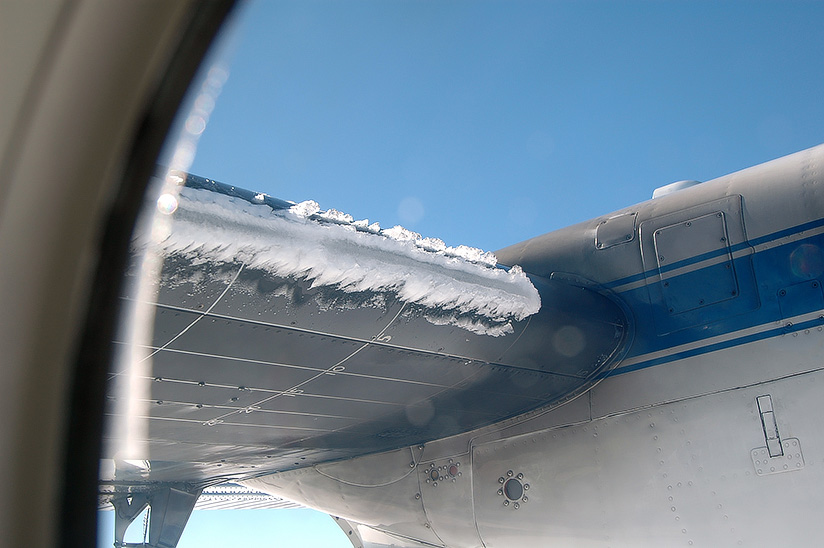
\includegraphics[
            width=6.8cm
        ]{FIGURES/SECTION_TRANSITION/ICE_WING.jpg}
    };
  \end{scope}
    \node[anchor=north,inner sep=0pt,font=\scriptsize,text=gray]
        at (2.75,-0.15) {Ice accretion on an aircraft wing*.};
\end{tikzpicture}

\end{column}
\hspace*{\fill}%

\end{columns}

\vspace{0.15cm}

% BOTTOM PHYSICAL PROCESS
\begin{center}
\vspace{-0.2cm}
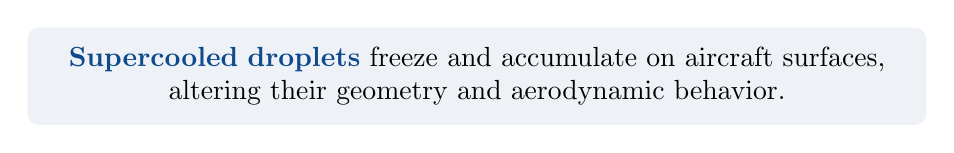
\begin{tikzpicture}

\node[
    fill=champsBlue!7,
    rounded corners=4pt,
    text width=0.9\textwidth+0.4cm,
    inner xsep=0.05cm, inner ysep=0.25cm,
    align=center
] {
    \textbf{\color{champsBlue}
    Supercooled droplets}
    freeze and accumulate on aircraft surfaces,\\
    altering their geometry and aerodynamic behavior.
};

\end{tikzpicture}
\end{center}

\vspace{-0.1cm}

\begin{columns}[T,onlytextwidth]

\begin{column}{0.48\textwidth}
\centering
{\color{champsBlue}\bfseries
Aerodynamic Performance Loss}

\vspace{0.08cm}
{\small Increased drag, reduced lift,\\
and degraded handling qualities}
\end{column}

\begin{column}{0.48\textwidth}
\centering
{\color{champsBlue}\bfseries
Flight Safety Risks}

\vspace{0.08cm}
{\small\justifying Potential loss of control
and catastrophic accidents}
\end{column}

\end{columns}

\begin{tikzpicture}[remember picture,overlay]
  \node[anchor=south west,font=\tiny,text=gray]
      at ([xshift=0.1cm,yshift=0.27cm]current page.south west)
      {*Image from Flight Society Foundation\quad\cite{CAO2018353,lynch2001effects,cao2015aircraft}};
\end{tikzpicture}

\end{frame}

% ---------------------------------------------------------------------------
% Slide 2: Aircraft Icing: Prediction and Certification
% ---------------------------------------------------------------------------
\begin{frame}{Aircraft Icing: Prediction and Certification}

\vspace{-0.15cm}

\noindent\resizebox{\textwidth}{!}{Accurate assessment of aircraft icing
is essential to demonstrate safe operation
under icing conditions.}

\vspace{0.05cm}
\vspace{0.25cm}
{\centering\color{champsBlue}\bfseries\large Three Complementary Approaches\par}
\vspace{0.1cm}

\vspace{-0.05cm}

\begin{columns}[T,onlytextwidth]

% FLIGHT TESTS
\begin{column}{0.32\textwidth}
\introCard
    {}
    {In-Flight Testing}
    {
    \textbf{Realistic operating conditions}

    \vspace{0.1cm}

    \textcolor{red!70!black}{\textbf{Limitations:}}

    High costs, safety risks, and
    limited control over atmospheric
    conditions.
    }
\end{column}

% WIND TUNNEL
\begin{column}{0.32\textwidth}
\introCard
    {}
    {Wind Tunnel Testing}
    {
    \textbf{Controlled experimental conditions}

    \vspace{0.1cm}

    \textcolor{red!70!black}{\textbf{Limitations:}}

    Scaling difficulties, facility
    constraints, and significant
    experimental costs.
    }
\end{column}

% NUMERICAL
\begin{column}{0.32\textwidth}
\introCard
    {}
    {Numerical Simulations}
    {
    \textbf{Flexible and cost-effective prediction}

    \vspace{0.1cm}

    \textcolor{champsBlue}{\textbf{Opportunities:}}

    Wider exploration of icing
    conditions and a growing role
    in certification activities.
    }
\end{column}

\end{columns}

\vspace{0.1cm}

\begin{center}
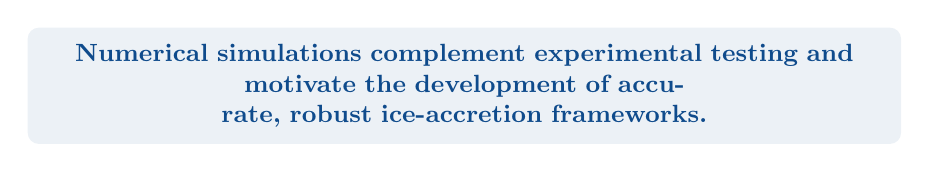
\begin{tikzpicture}
\node[fill=champsBlue!8, rounded corners=4pt,
      text width=0.88\textwidth, inner sep=6pt,
      align=center, font=\small] {%
\textbf{\color{champsBlue}
Numerical simulations complement experimental
testing and\\ motivate the development of
accurate, robust ice-accretion frameworks.}
};
\end{tikzpicture}
\end{center}

\SlideRef{FAAAppendixC,FAAAppendixO,potapczuk2013aircraft,wright2008user}
\end{frame}

% ---------------------------------------------------------
% Separation of physical time scales
% ---------------------------------------------------------
\begin{frame}{Separation of Physical Time Scales}

\vspace{0.1cm}

\noindent\resizebox{\textwidth}{!}{Aircraft icing involves physical processes operating
at significantly different characteristic time scales.}

\vspace{0.15cm}

\begin{center}
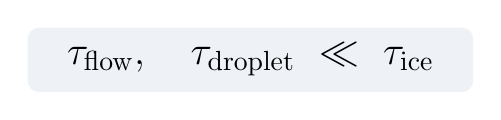
\begin{tikzpicture}
\node[fill=champsBlue!7, rounded corners=4pt, inner xsep=0.5cm, inner ysep=0.2cm] {%
{\Large
$\displaystyle
\tau_{\mathrm{flow}},
\quad \tau_{\mathrm{droplet}}
\ \ll\
\tau_{\mathrm{ice}}
$}};
\end{tikzpicture}

\vspace{0.7cm}
$\displaystyle
\tau_{\mathrm{flow}}=\frac{L}{U_\infty}\sim\mathcal{O}(10^{-2}\,\mathrm{s}),\qquad
\tau_{\mathrm{droplet}}=\frac{\rho_d D^2}{18\mu_a}\sim\mathcal{O}(10^{-3}\,\mathrm{s}),\qquad
\tau_{\mathrm{ice}}=\frac{L}{V_{\mathrm{ice}}}\sim\mathcal{O}(10^{5}\,\mathrm{s})$
\end{center}

\vspace{0.2cm}

\begin{center}
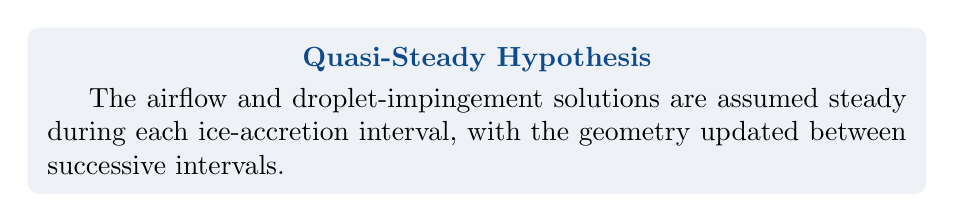
\begin{tikzpicture}
\node[
    fill=champsBlue!7,
    rounded corners=4pt,
    text width=0.9\textwidth,
    inner sep=0.25cm,
    align=justify
] {
    \centering{\color{champsBlue}\bfseries Quasi-Steady Hypothesis}\\[0.1cm]\justifying
    The airflow and droplet-impingement solutions are
    assumed steady during each ice-accretion interval,
    with the geometry updated between successive intervals.
};
\end{tikzpicture}
\end{center}

\SlideRef{guardoneReview}
\end{frame}

% ---------------------------------------------------------
% Quasi-steady ice-accretion workflow
% ---------------------------------------------------------
\begin{frame}{Numerical Ice-Accretion Modeling}

\begin{columns}[c,onlytextwidth]

% LEFT: steps, highlighted one at a time
\begin{column}{0.58\textwidth}
\IcingText{01 \quad Geometry and Mesh Representation}
{Definition of the initial geometry using
a \textbf{body-fitted} or
\textbf{immersed-boundary} approach.}\par\vspace{0.22cm}
\IcingText{02 \quad Aerodynamic Flow}
{Air velocity $\mathbf{u}_a$, pressure $p$,
temperature $T$, and heat-transfer
coefficient (HTC).}\par\vspace{0.22cm}
\IcingText{03 \quad Droplet Impingement}
{Droplet trajectories and collection
efficiency $\beta$, yielding the
impinging water mass flux
$\dot{m}_{\mathrm{imp}}$.}\par\vspace{0.22cm}
\IcingText{04 \quad Thermodynamics and Ice Growth}
{Surface mass and energy balances
yielding the ice accretion rate
$\dot{m}_{\mathrm{ice}}$ and
ice thickness $h_{\mathrm{ice}}$.}\par\vspace{0.22cm}
\IcingText{05 \quad Geometry and Mesh Update}
{Update the ice geometry and adapt
the computational representation
for the next accretion step.}
\end{column}

% RIGHT: one image at a time, centred
\begin{column}{0.40\textwidth}
\centering
\only<1>{%
  {\scriptsize\color{champsBlue}\bfseries Body-fitted}\par\vspace{0.05cm}
  {\setlength{\fboxsep}{0pt}\setlength{\fboxrule}{0.6pt}\fbox{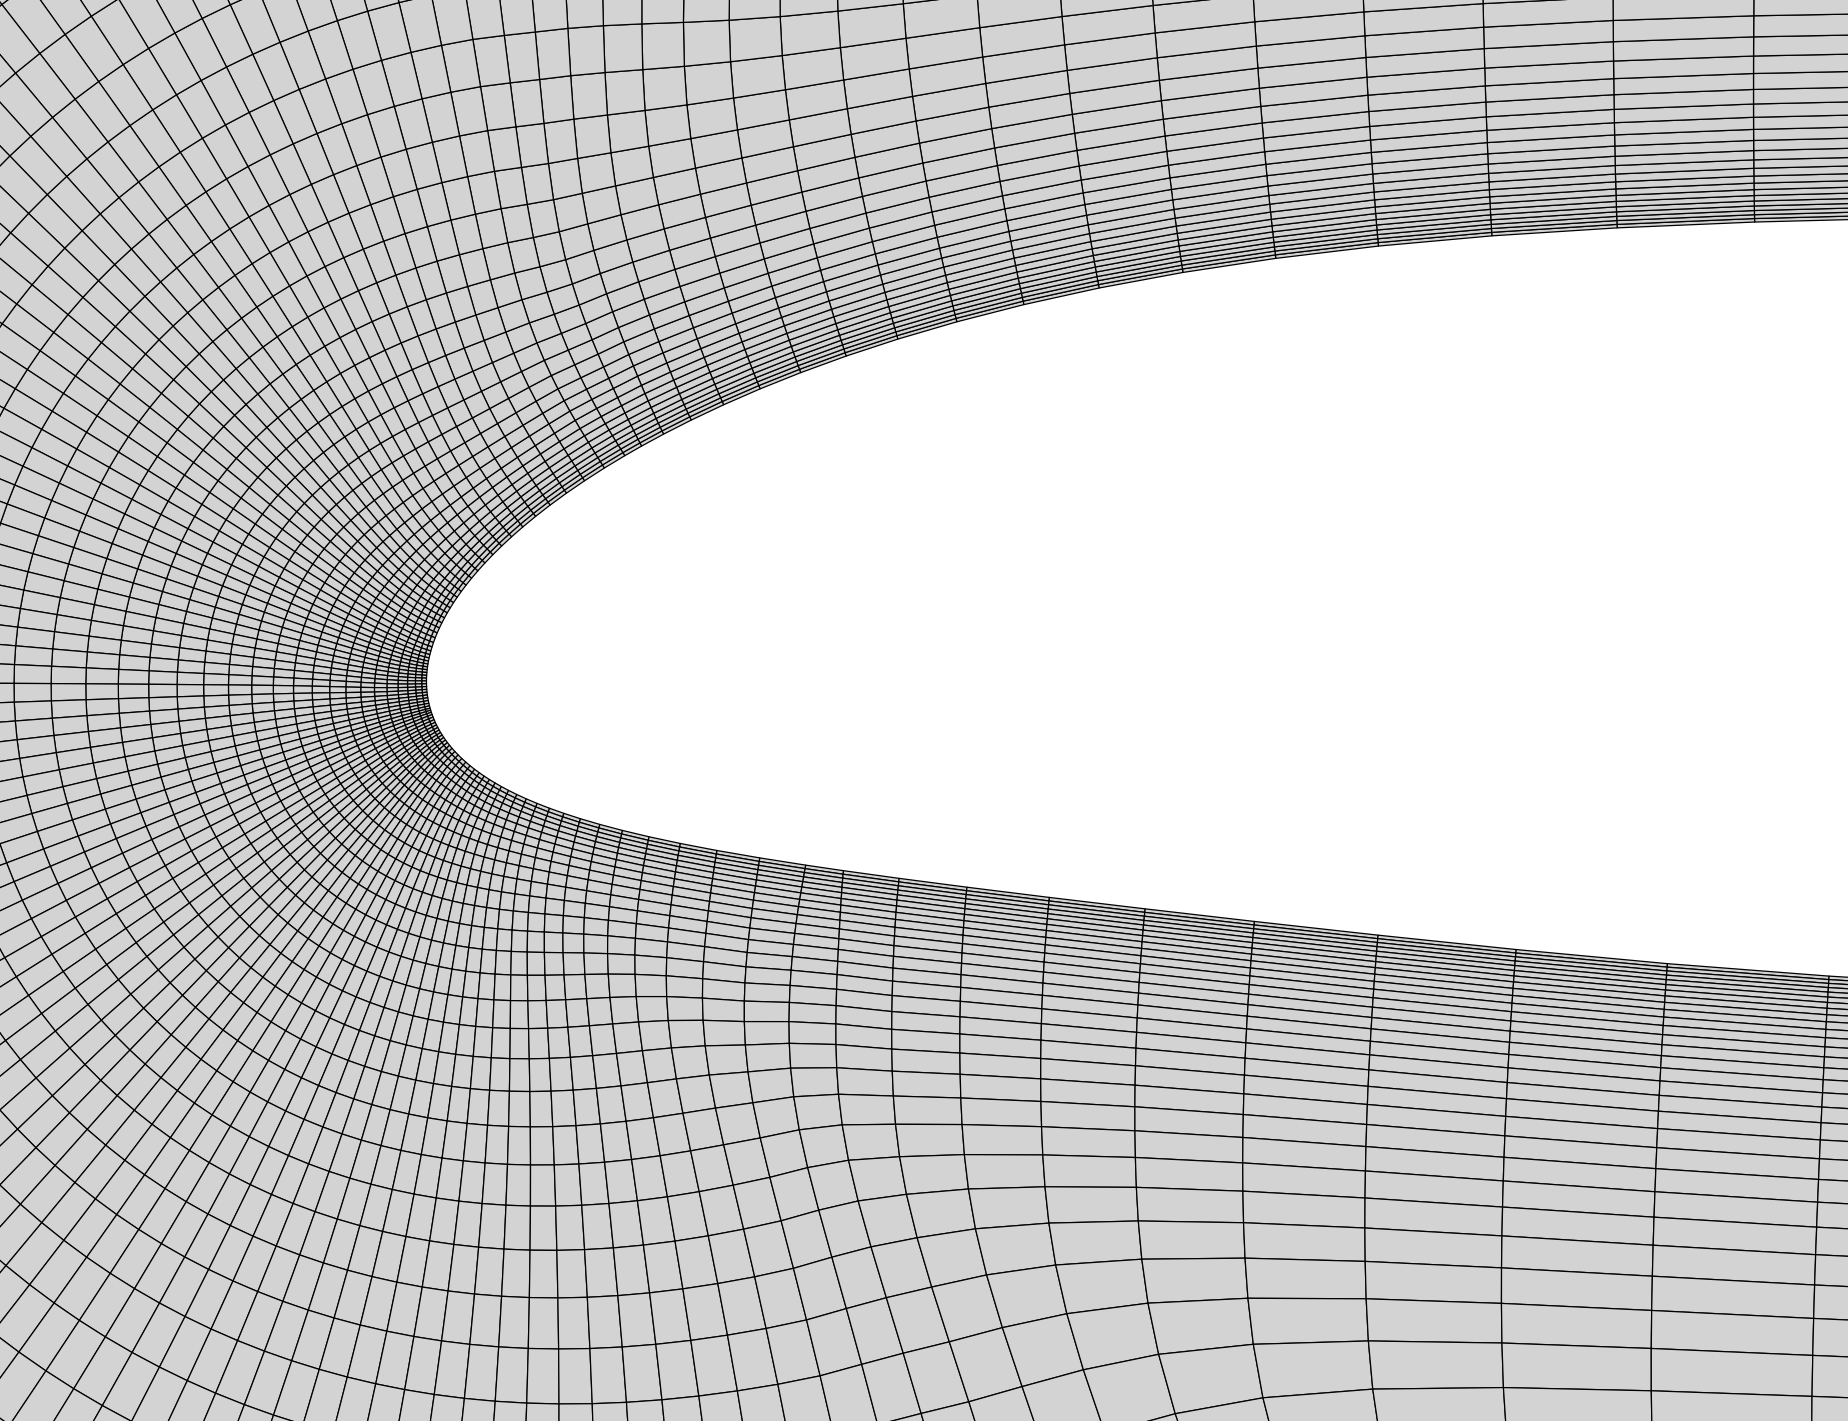
\includegraphics[width=\linewidth,height=2.95cm,keepaspectratio]{FIGURES/INTRODUCTION/meshLE_BF}}}\par\vspace{0.08cm}
  {\scriptsize\color{champsBlue}\bfseries Immersed boundary}\par\vspace{0.05cm}
  {\setlength{\fboxsep}{0pt}\setlength{\fboxrule}{0.6pt}\fbox{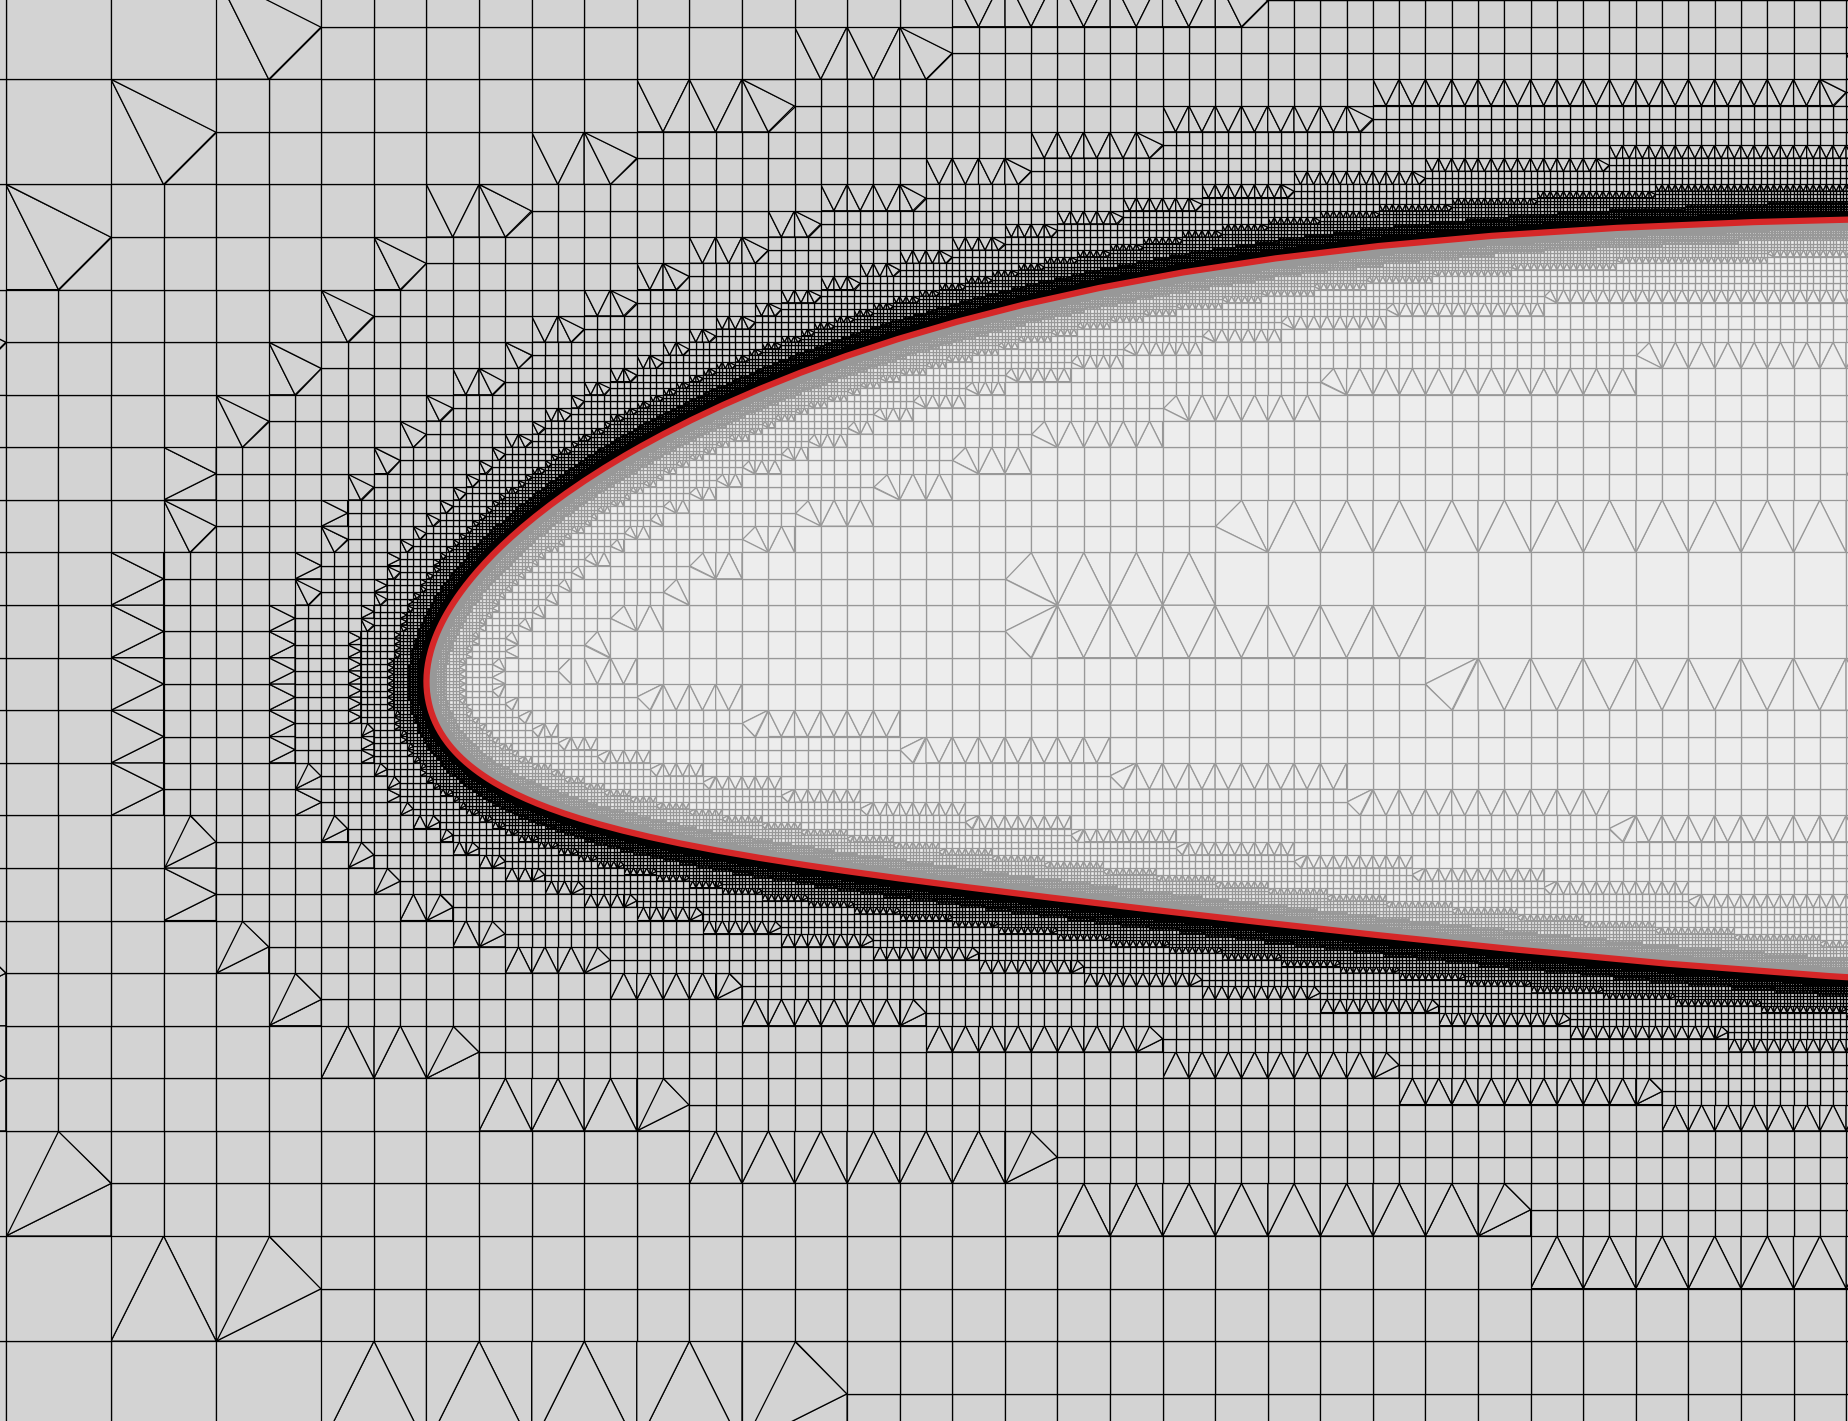
\includegraphics[width=\linewidth,height=2.95cm,keepaspectratio]{FIGURES/INTRODUCTION/meshLE_IBM}}}}%
\only<2>{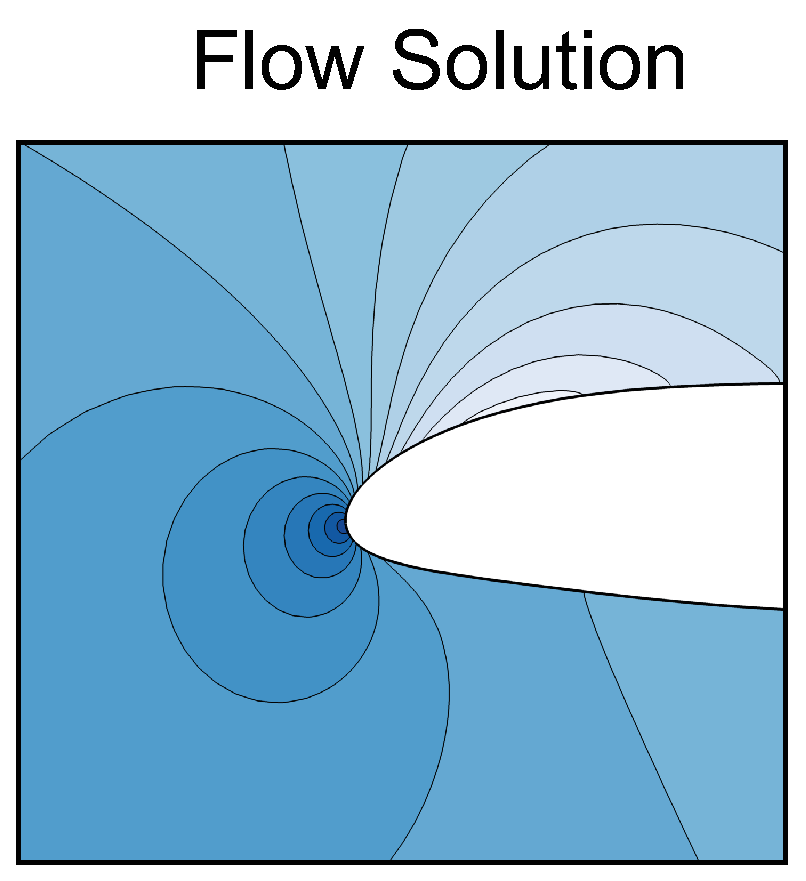
\includegraphics[width=\linewidth,height=4.4cm,keepaspectratio,trim=0 0 0 56,clip]{FIGURES/INTRODUCTION/FLOW}}%
\only<3>{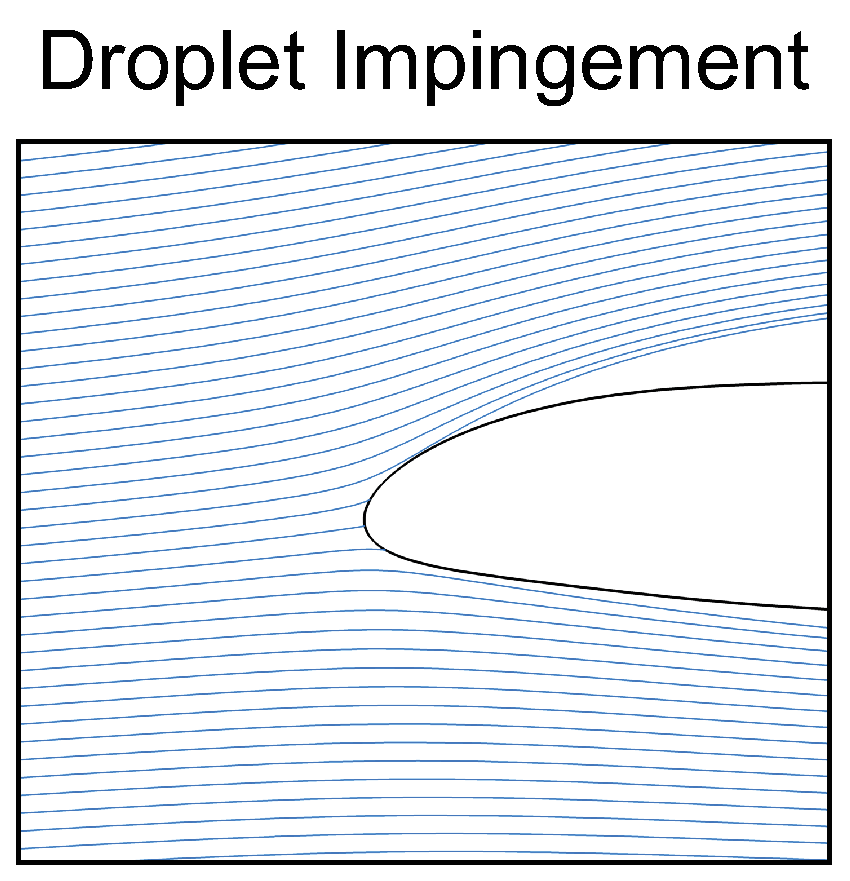
\includegraphics[width=\linewidth,height=4.4cm,keepaspectratio,trim=0 0 0 56,clip]{FIGURES/INTRODUCTION/DROPLET}}%
\only<4>{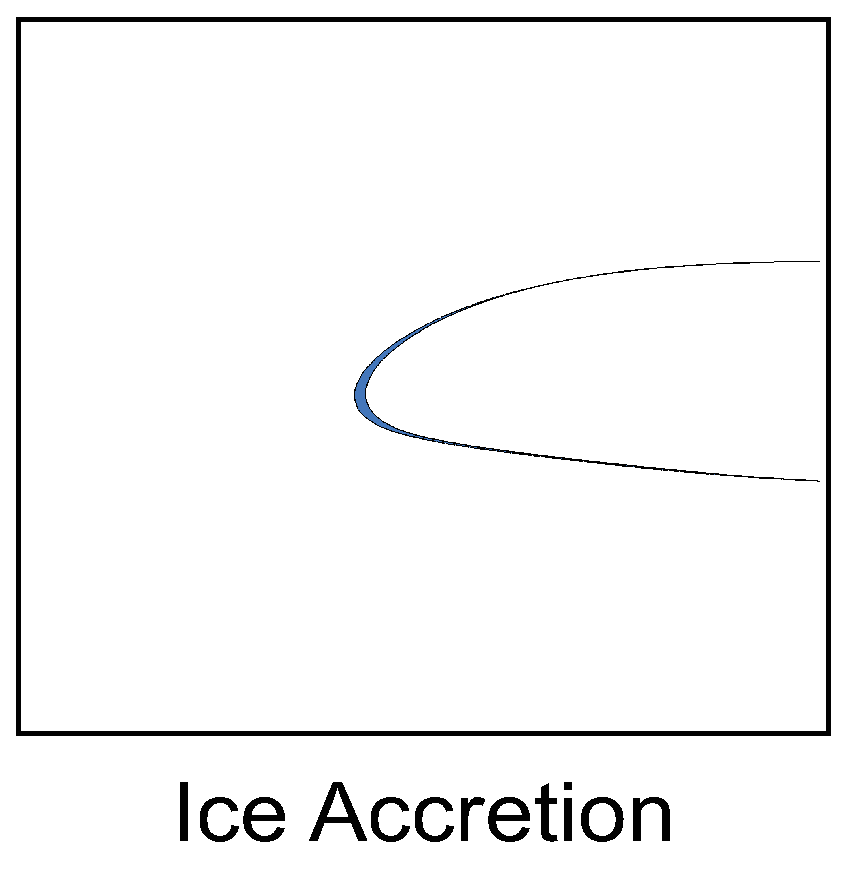
\includegraphics[width=\linewidth,height=4.4cm,keepaspectratio,trim=0 62 0 0,clip]{FIGURES/INTRODUCTION/ACCRETION}}%
\only<5>{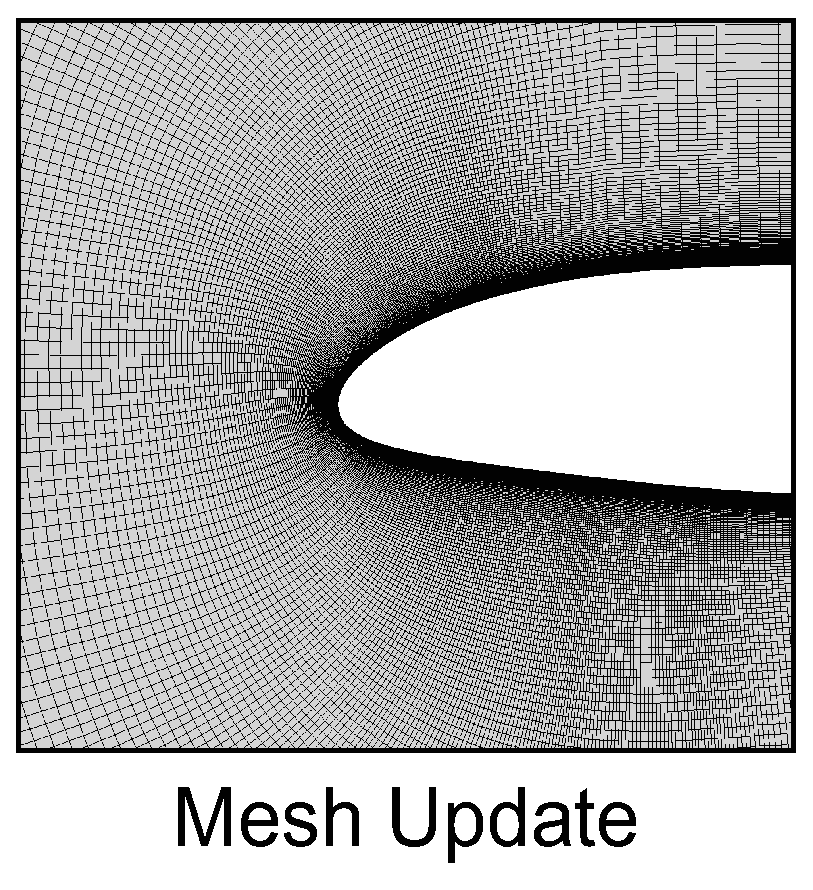
\includegraphics[width=\linewidth,height=4.4cm,keepaspectratio,trim=0 57 0 0,clip]{FIGURES/INTRODUCTION/UPDATE}}%
\end{column}

\end{columns}

\SlideRef{messingerClassical,guardoneReview}
\end{frame}

\begin{frame}{Quasi-Steady Ice-Accretion Framework}
\vspace{-0.15cm}
\begin{center}
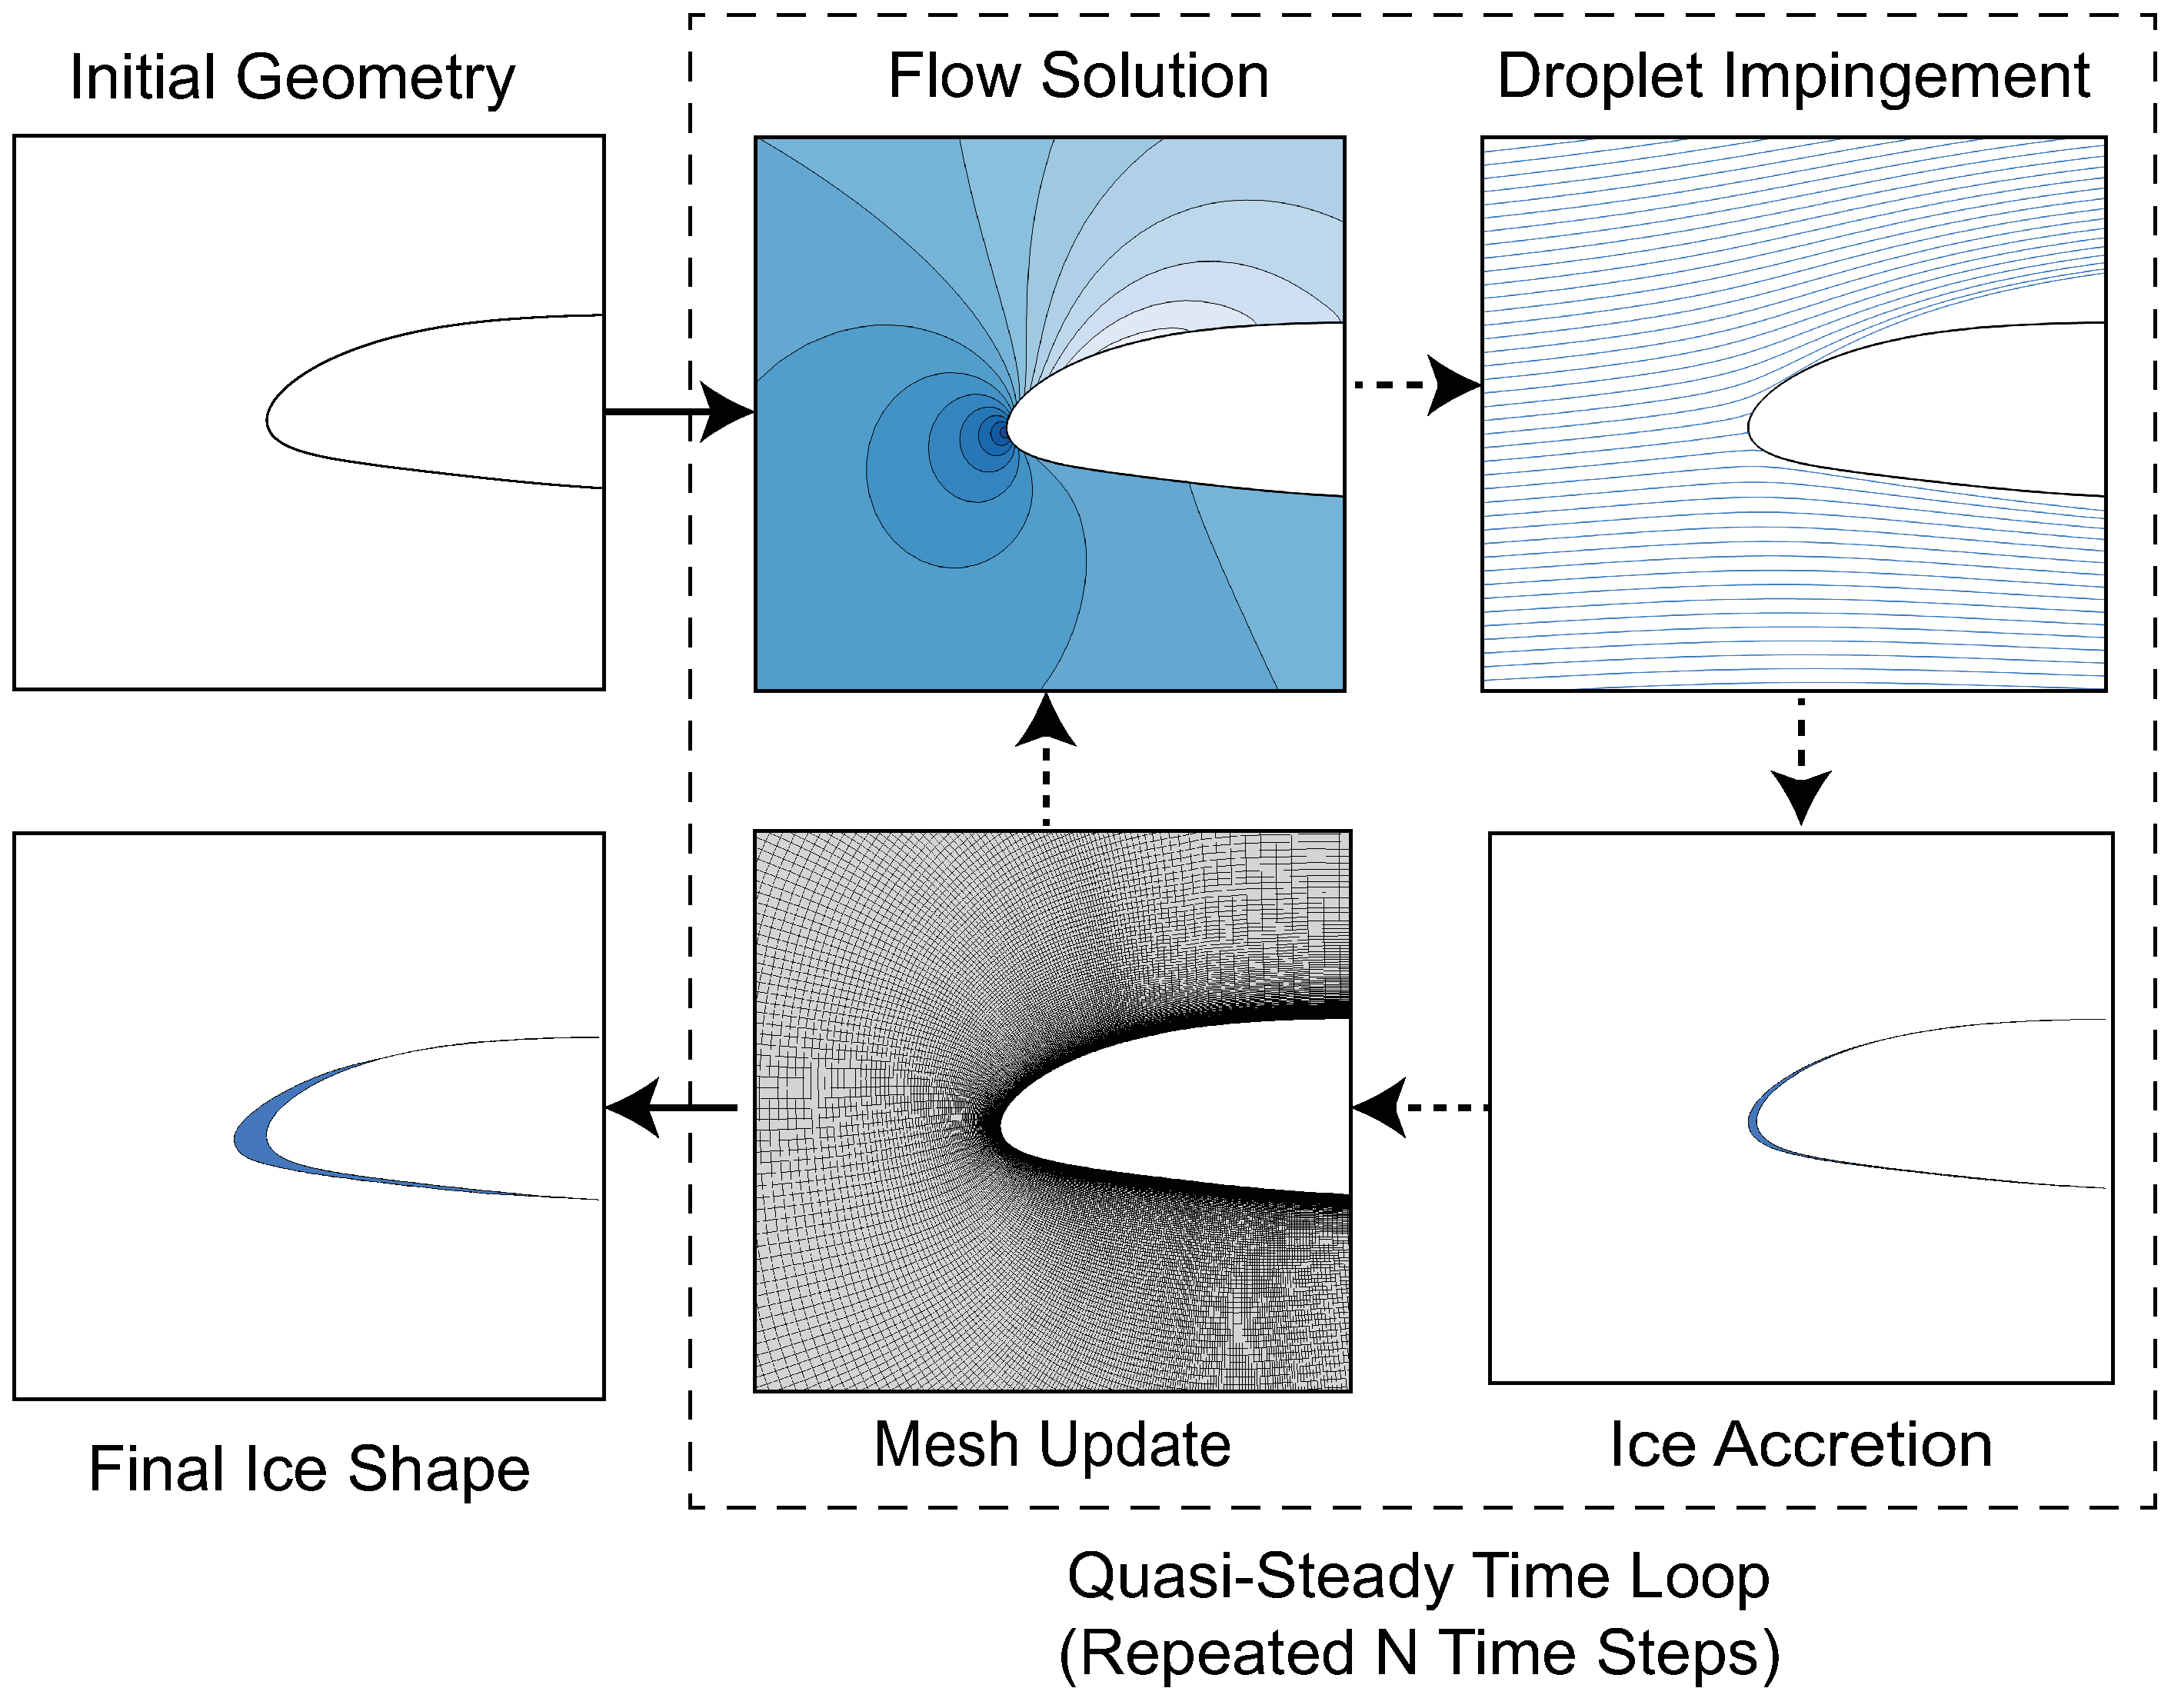
\includegraphics[width=\textwidth,height=0.90\textheight,keepaspectratio]{FIGURES/INTRODUCTION/ICING_FRAMEWORK}
\end{center}
\SlideRef{radenac2024workflow,guardoneReview}
\end{frame}

% ---------------------------------------------------------
% Single-step vs. multilayer ice accretion
% ---------------------------------------------------------
\begin{frame}{Single-Step vs. Multilayer Ice Accretion}
\vspace{0.12cm}
\begin{columns}[T,onlytextwidth]
 \begin{column}{0.485\textwidth}
  \centering
  {\color{champsBlue}\bfseries Single-step ($N=1$)}\par
  \vspace{0.20cm}
  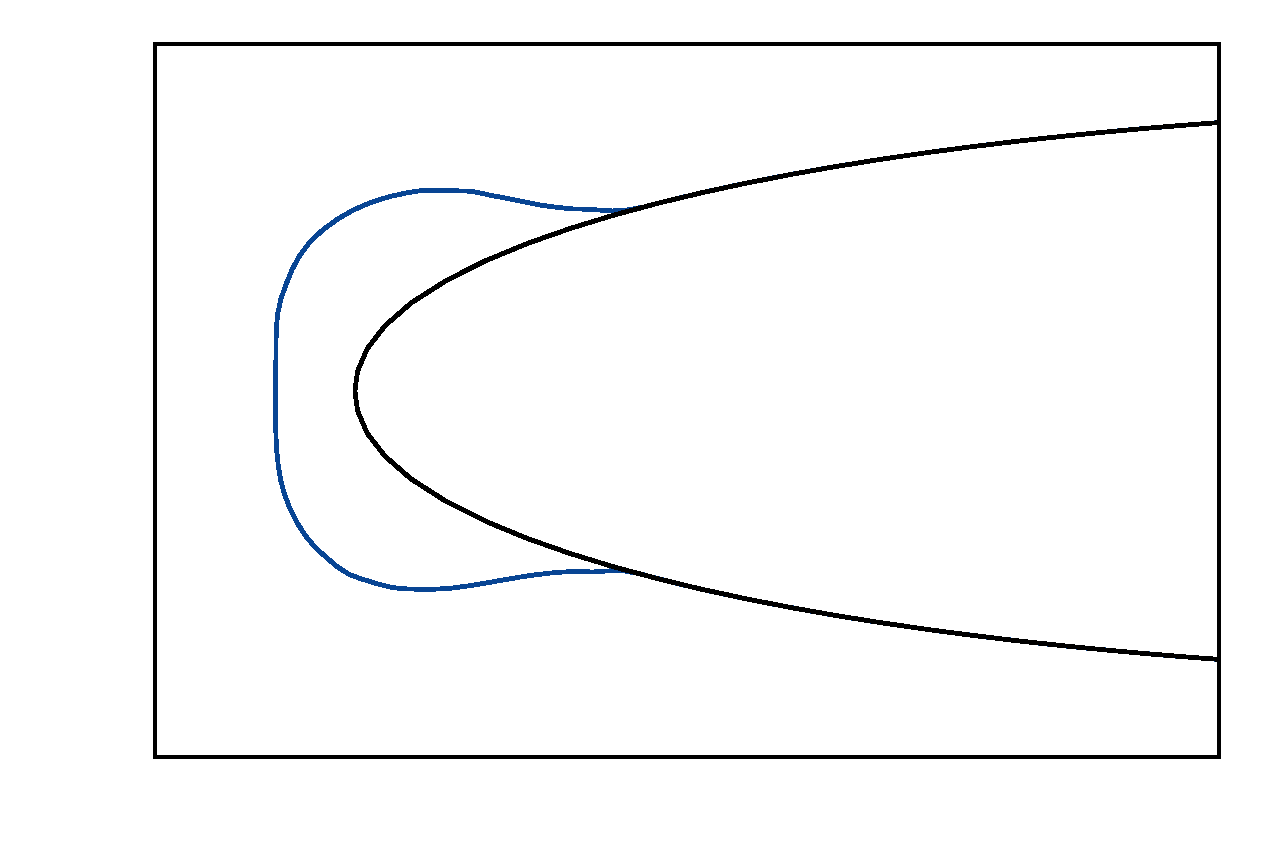
\includegraphics[width=0.98\linewidth,height=3.55cm,keepaspectratio]
    {FIGURES/INTRODUCTION/CASE_362_IPW1_SINGLE_LAYER}\par
  \vspace{0.18cm}
  {\small One accretion interval using the initial aerodynamic and impingement fields.}
 \end{column}
 \begin{column}{0.485\textwidth}
  \centering
  {\color{champsBlue}\bfseries Multilayer ($N=5$)}\par
  \vspace{0.20cm}
  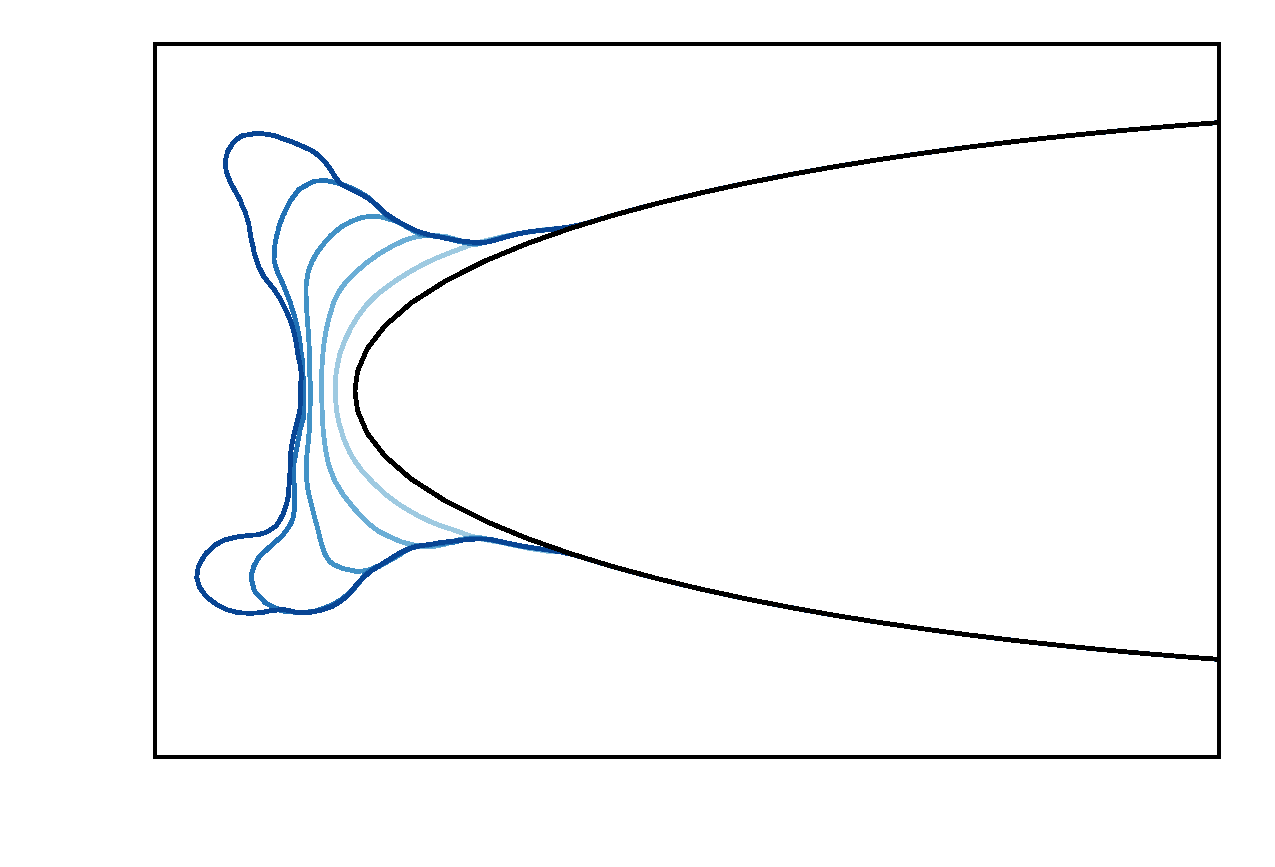
\includegraphics[width=0.98\linewidth,height=3.55cm,keepaspectratio]
    {FIGURES/INTRODUCTION/CASE_362_IPW1_FIVE_LAYERS}\par
  \vspace{0.18cm}
  {\small Repeated geometry updates and recomputation of the coupled fields.}
 \end{column}
\end{columns}
\vfill
\begin{center}

\begin{tikzpicture}
\node[fill=champsBlue!5, draw=champsBlue!18, rounded corners=4pt,
      text width=0.90\textwidth, inner sep=3pt, align=center, font=\small] {%
  \textbf{Geometry feedback matters:} multilayer simulations can capture the development of more complex ice features.};
\end{tikzpicture}
\end{center}
\SlideRef{bourgault-coteMultilayerAirfoilIce2019,radenac2024workflow}
\end{frame}

\begin{frame}{Ice Accretion: Key Terminology}

\vspace{0.15cm}

{\small Ice morphology depends on atmospheric and
aerodynamic conditions and the local freezing process.\par}

\vspace{0.05cm}

\begin{columns}[T,onlytextwidth]

% RIME ICE
\begin{column}{0.315\textwidth}
\centering
{\color{champsBlue}\bfseries\large Rime Ice}

\vspace{0.02cm}

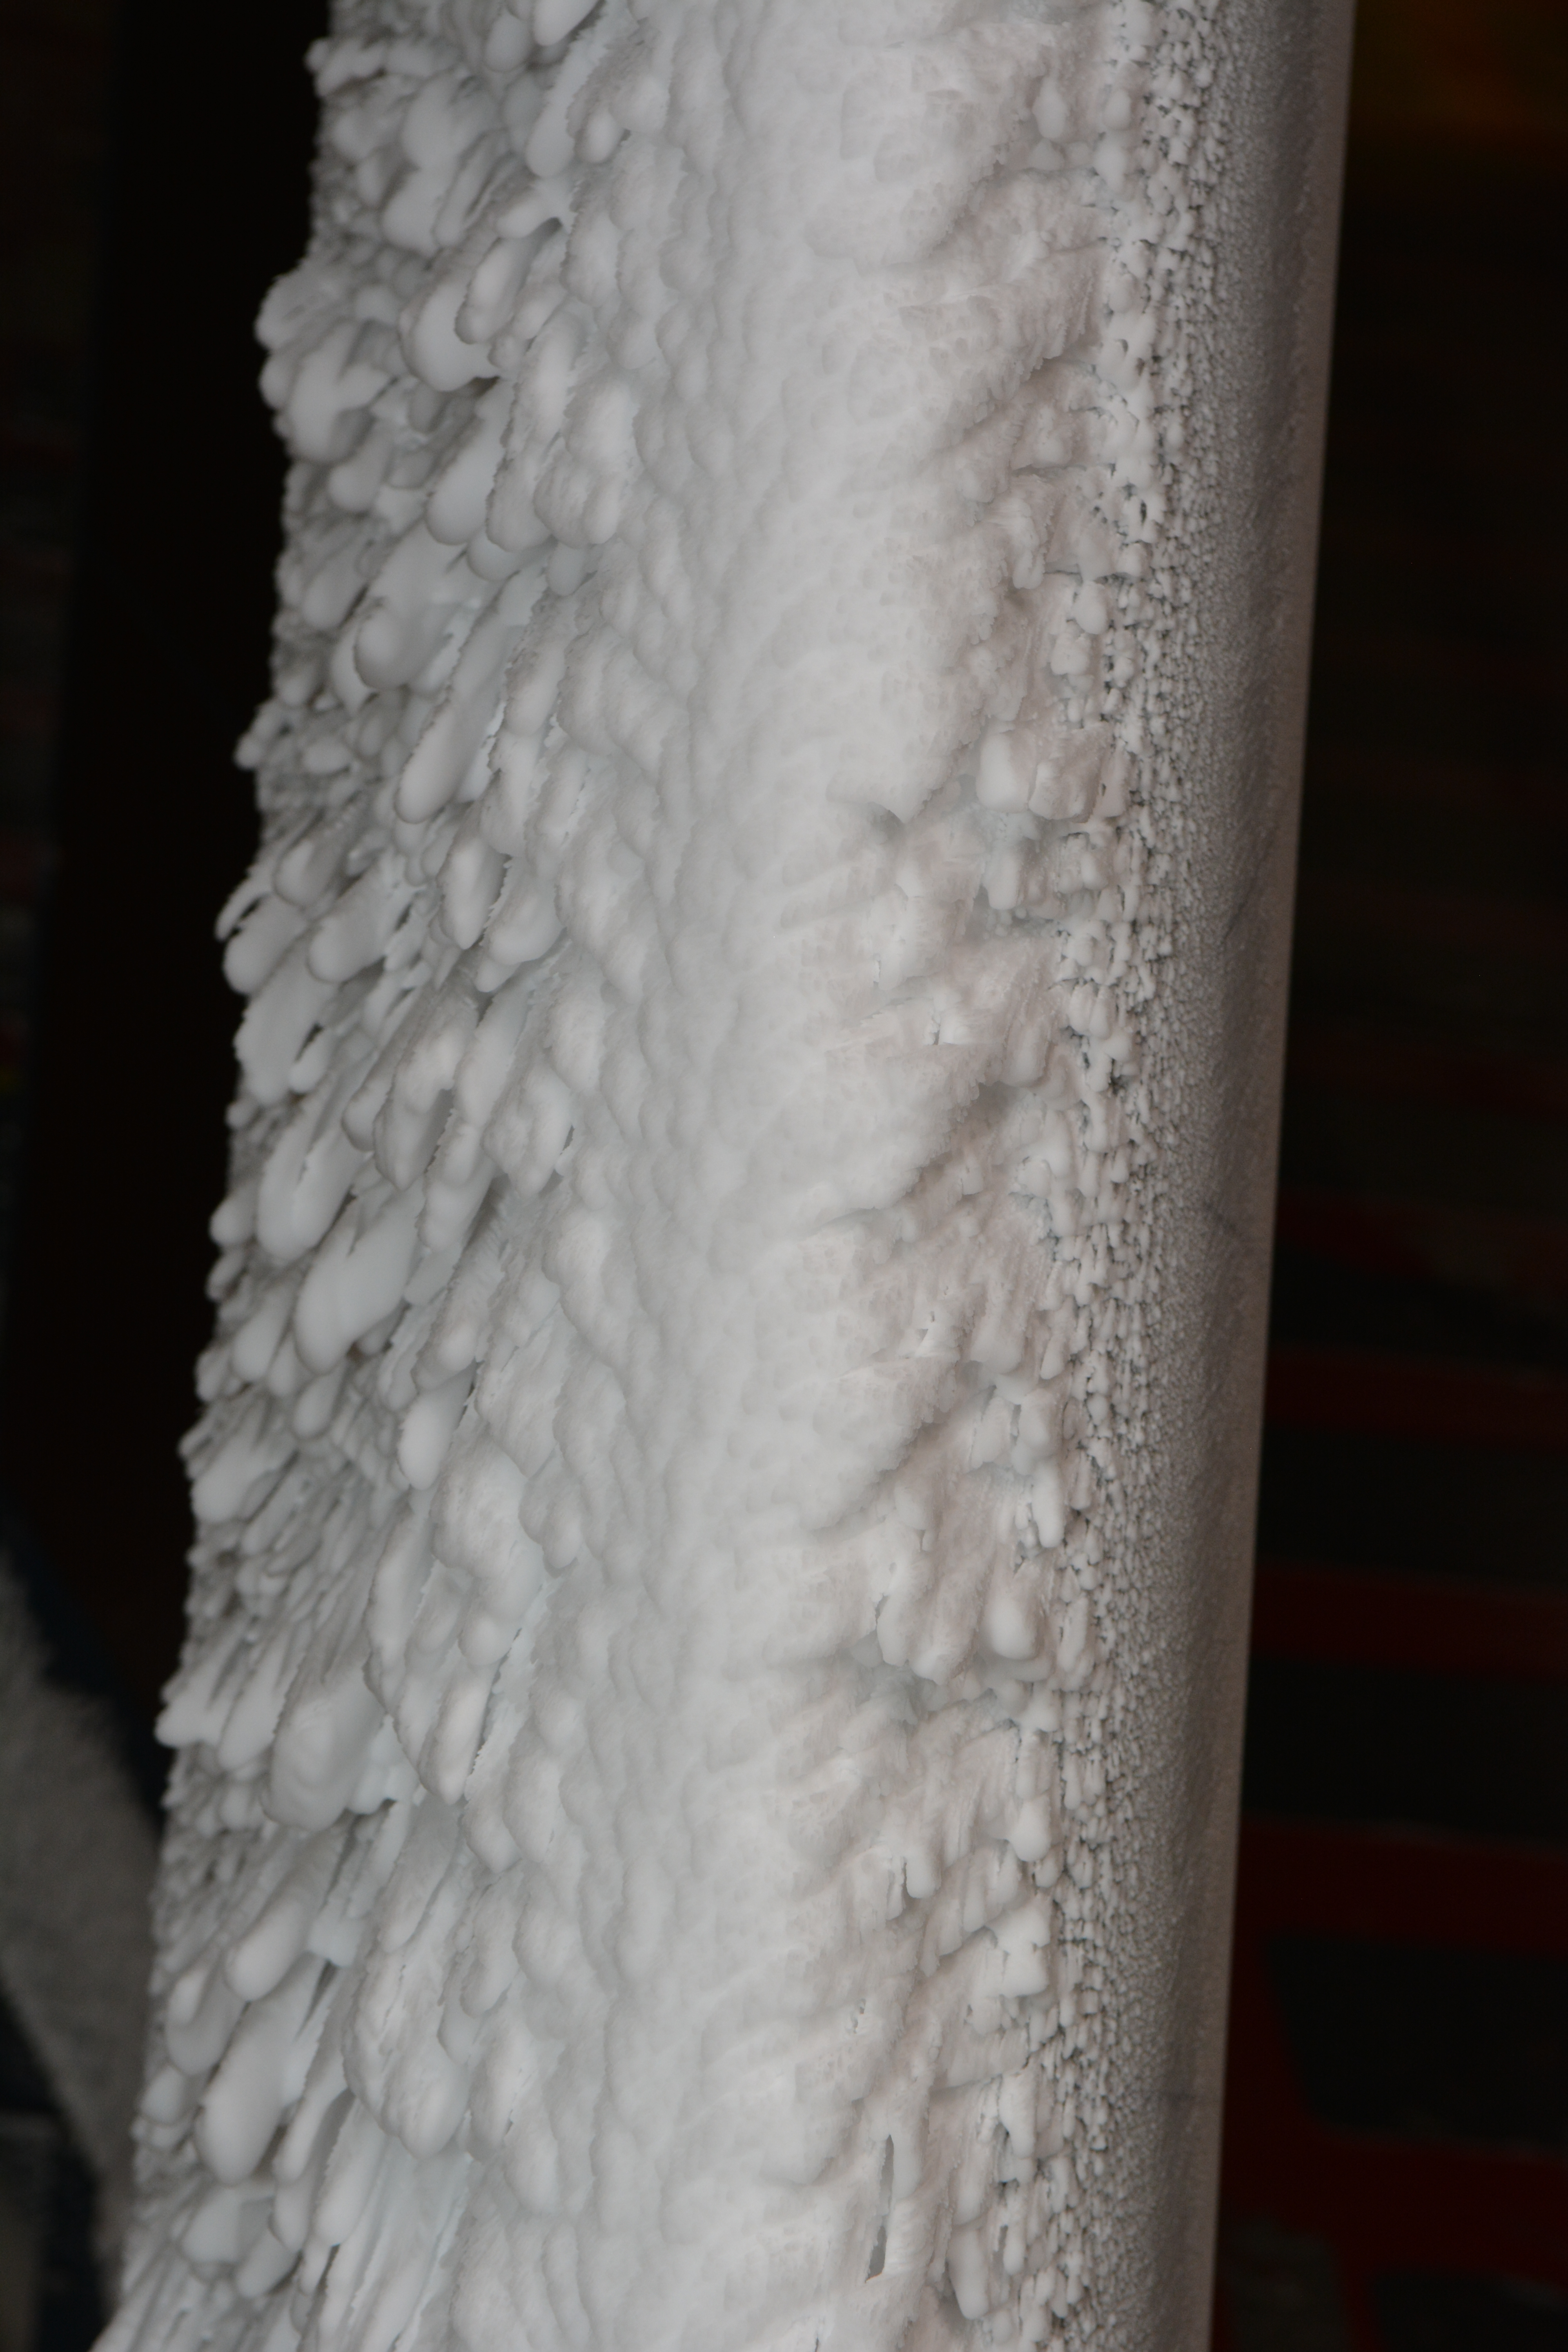
\includegraphics[width=\linewidth,height=3.3cm,keepaspectratio]{FIGURES/INTRODUCTION/CRM_RIME.JPG}

\vspace{0.02cm}

{\footnotesize
Rapid freezing upon impact, producing
streamlined, opaque ice deposits.\par}
\end{column}

% MIXED ICE
\begin{column}{0.315\textwidth}
\centering
{\color{champsBlue}\bfseries\large Mixed Ice}

\vspace{0.02cm}

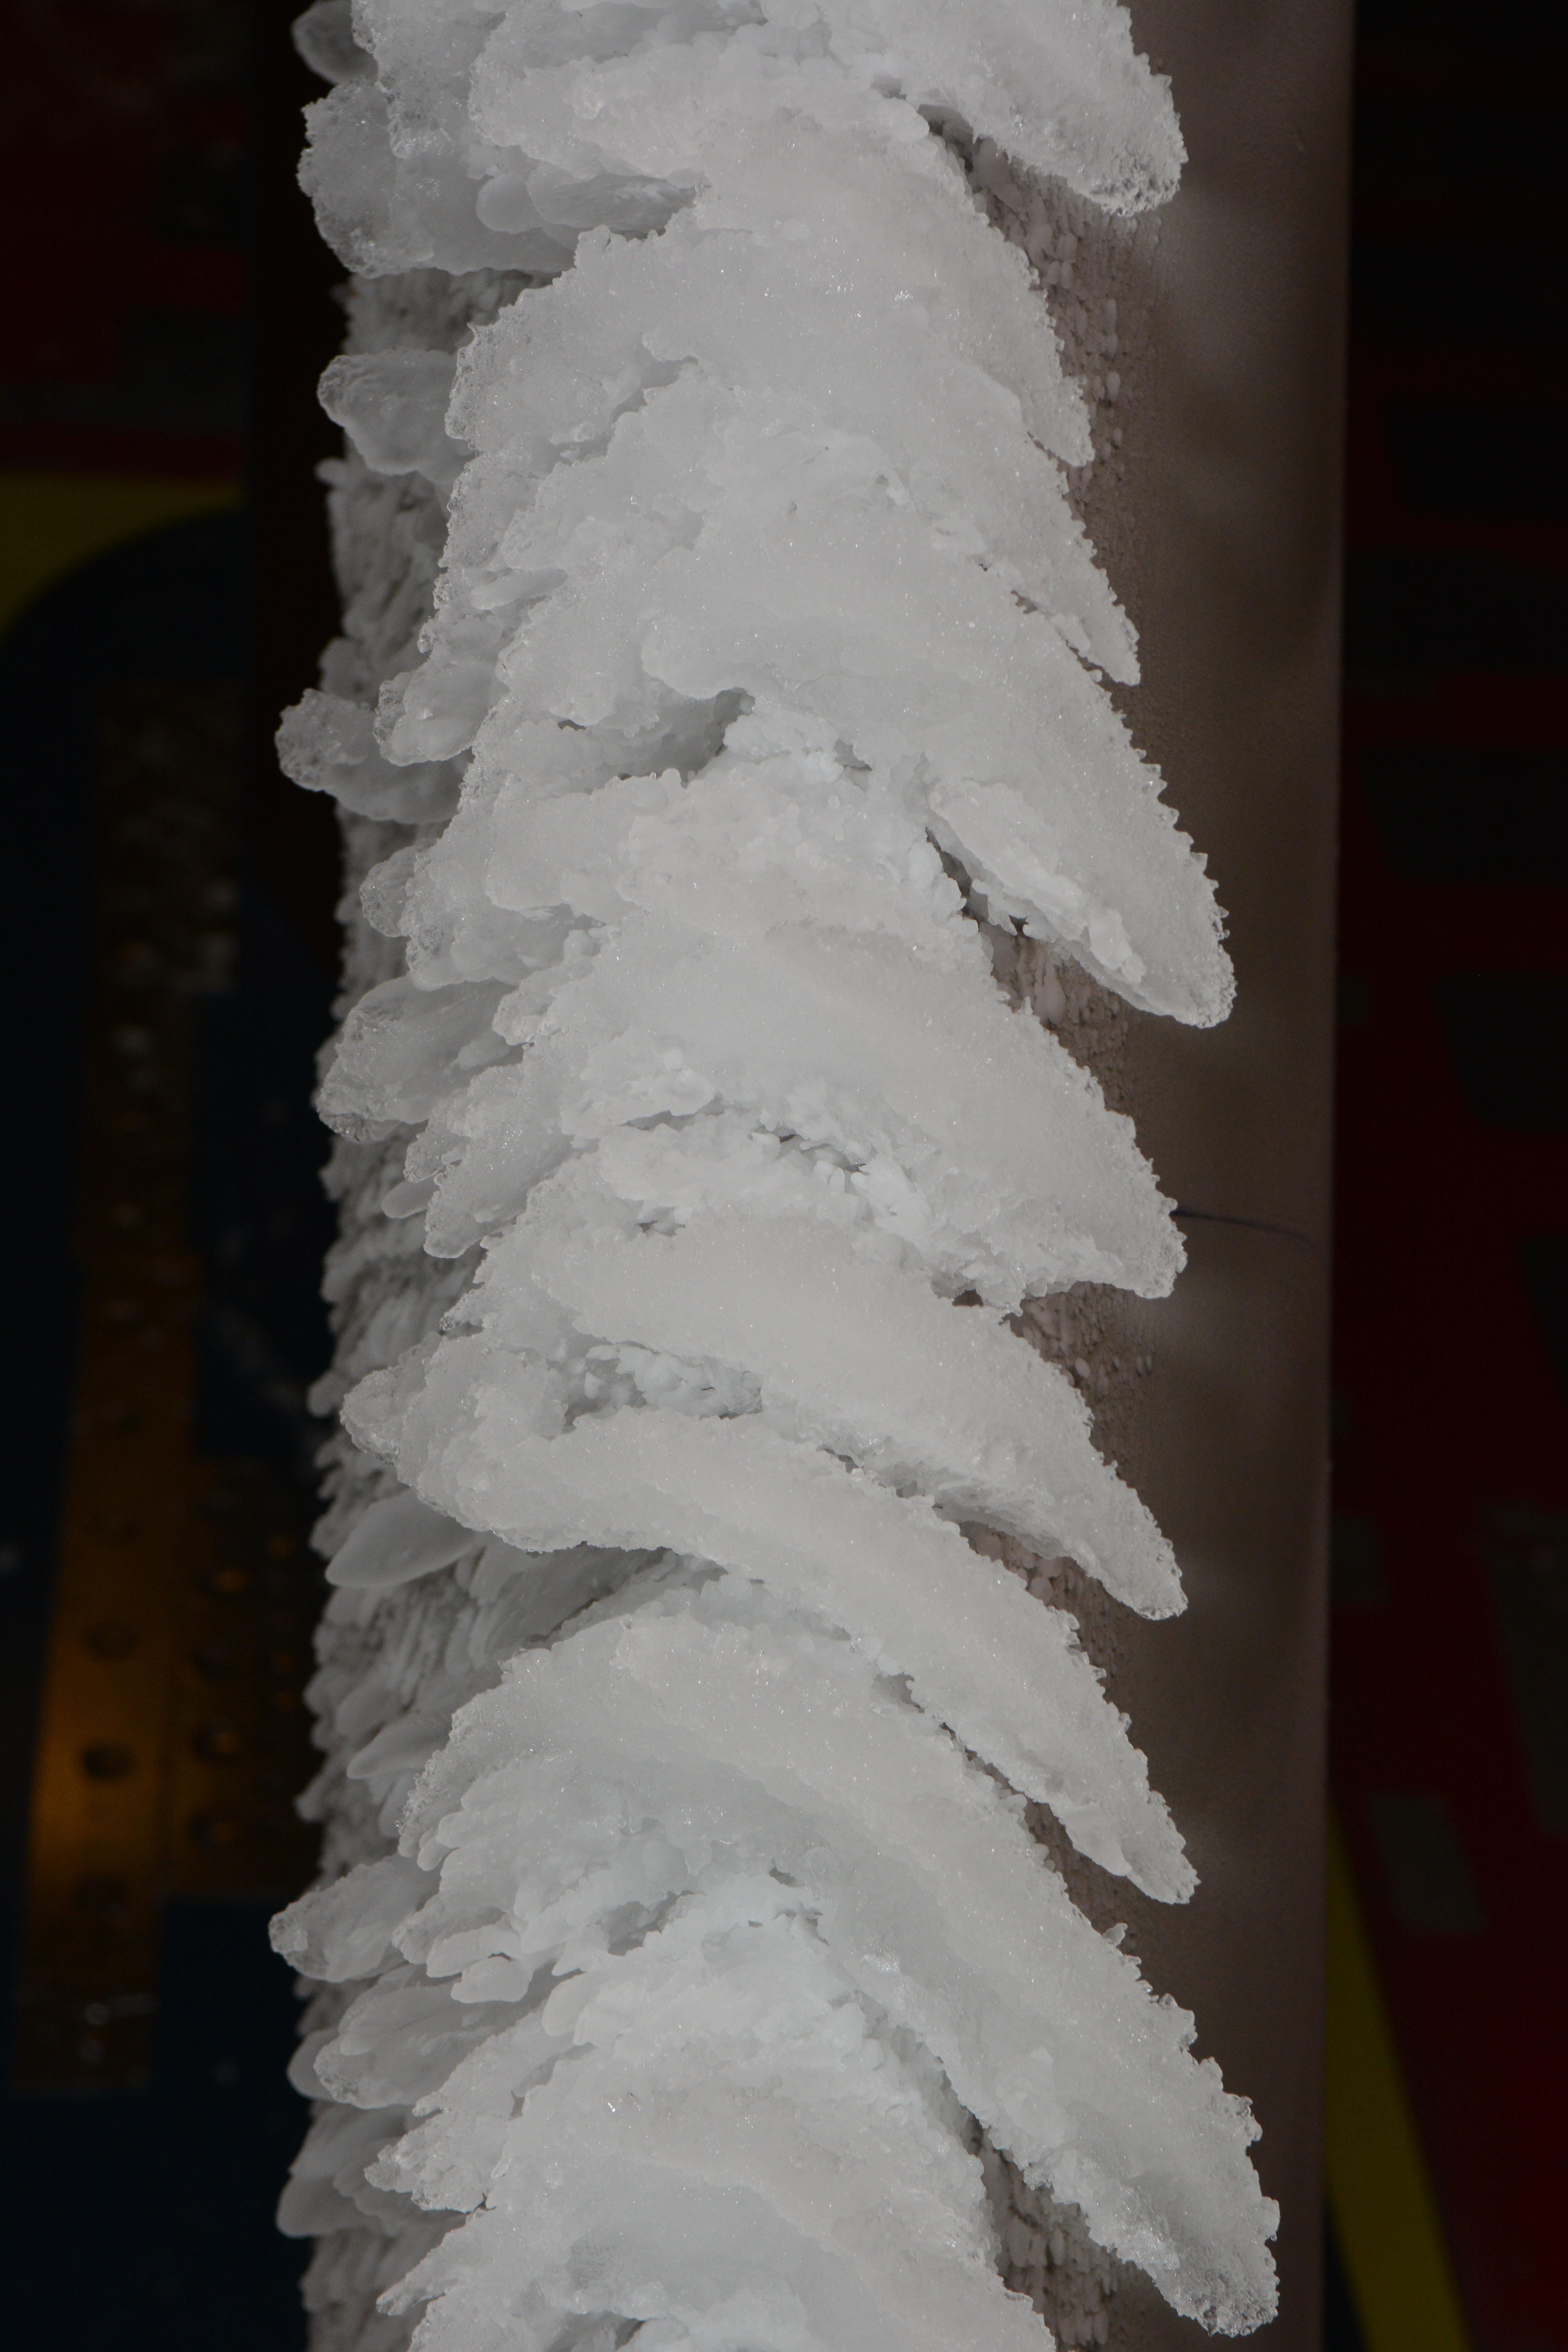
\includegraphics[width=\linewidth,height=3.3cm,keepaspectratio]{FIGURES/INTRODUCTION/CRM_MIXED.JPG}

\vspace{0.02cm}

{\footnotesize
Combination of rime- and glaze-like
ice characteristics.\par}
\end{column}

% GLAZE ICE
\begin{column}{0.315\textwidth}
\centering
{\color{champsBlue}\bfseries\large Glaze Ice}

\vspace{0.02cm}

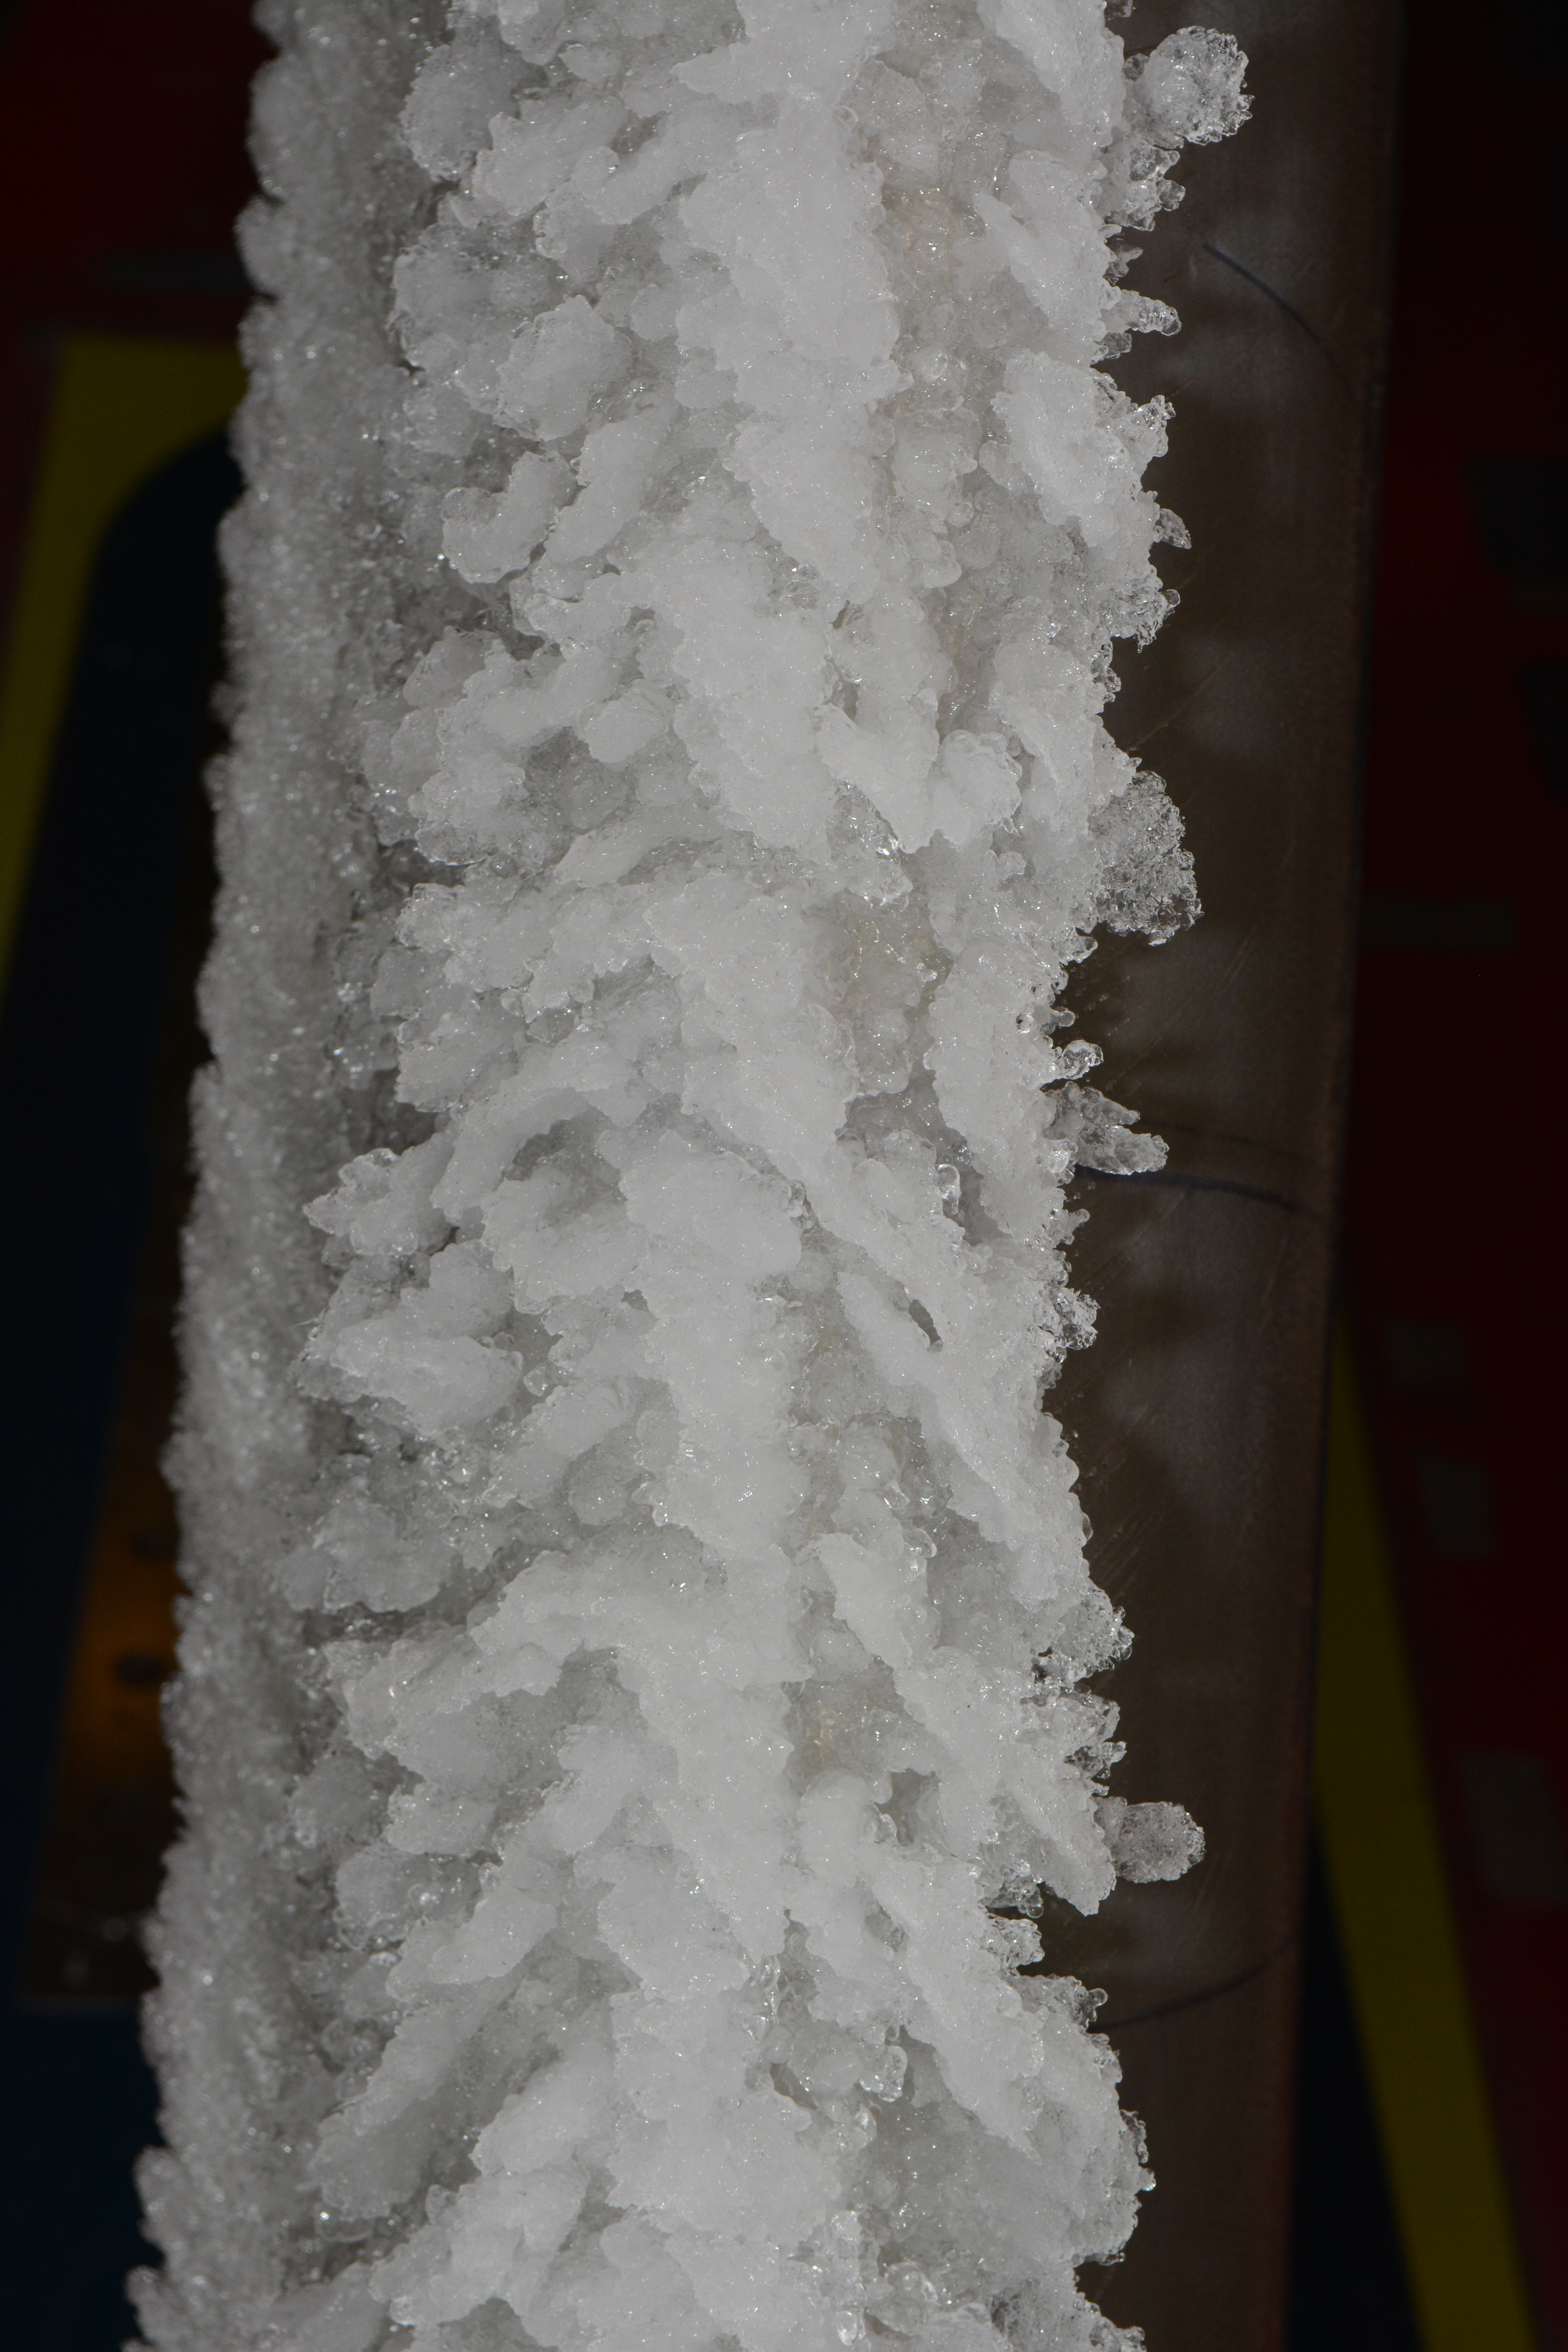
\includegraphics[width=\linewidth,height=3.3cm,keepaspectratio]{FIGURES/INTRODUCTION/CRM_GLAZE.JPG}

\vspace{0.02cm}

{\footnotesize
Partial freezing with liquid-water runback,
often resulting in complex horn-like shapes.\par}
\end{column}

\end{columns}

\vspace{0.15cm}
\noindent
\begin{tikzpicture}
\useasboundingbox (0,-0.12) rectangle (\textwidth,0.12);
\shade[left color=blue!70!black, right color=red!80!black]
  (0.16\textwidth,-0.6pt) rectangle (0.83\textwidth,0.6pt);
\fill[red!80!black] (0.83\textwidth,-3pt) -- (0.845\textwidth,0) -- (0.83\textwidth,3pt) -- cycle;
\node[fill=white, inner xsep=4pt, inner ysep=1pt, font=\scriptsize\bfseries, text=champsBlue]
  at (0.5\textwidth,0) {Increasing Ambient Temperature};
\end{tikzpicture}\par
\vspace{0.08cm}

\justifying{\color{champsBlue}\bfseries
Supercooled Large Droplets (SLD):}
{\small
Large droplets that may splash, rebound,
and reimpinge downstream. SLD-related accidents motivated their inclusion
in aircraft certification requirements (Appendix O).\par}

\begin{tikzpicture}[remember picture,overlay]
  \node[anchor=south west,font=\tiny,text=gray]
      at ([xshift=0.1cm,yshift=0.27cm]current page.south west)
      {Images from 2nd Ice Prediction Workshop~\cite{laurendeau2024summary}\quad\cite{FAAAppendixO}};
\end{tikzpicture}

\end{frame}

% ---------------------------------------------------------
% Challenges in 3D multilayer ice accretion
% ---------------------------------------------------------
\begin{frame}{Challenges in Multilayer Ice Accretion}

\vspace{0.1cm}

\begin{columns}[c,onlytextwidth]

% LEFT: challenges, highlighted one at a time
\begin{column}{0.54\textwidth}
\IcingText{01 \quad Droplet Impingement}
{Lagrangian tracking naturally captures individual
droplet dynamics and enables SLD modeling.
\textbf{How can it remain efficient and scalable
for complex 3D configurations?}}
\par\vspace{0.2cm}

\IcingText{02 \quad Geometry Evolution}
{Direct surface-node displacement can lead to
mesh degradation and entanglement.
\textbf{How can complex 3D ice geometries be evolved
robustly over successive accretion layers?}}
\par\vspace{0.2cm}

\IcingText{03 \quad Geometry Representation}
{Body-fitted approaches require repeated
flow-mesh deformation or remeshing.
\textbf{How can immersed-boundary methods reduce
these constraints while achieving comparable accuracy?}}
\end{column}

% RIGHT: one illustration per challenge
\begin{column}{0.43\textwidth}
\centering
\parbox[c][6.6cm][c]{\linewidth}{\centering
\only<1>{%
  {\scriptsize\color{champsBlue}\bfseries Lagrangian droplet tracking}\par\vspace{0.05cm}
  \movie[width=\linewidth,height=0.5625\linewidth,poster,showcontrols,loop,autostart]%
    {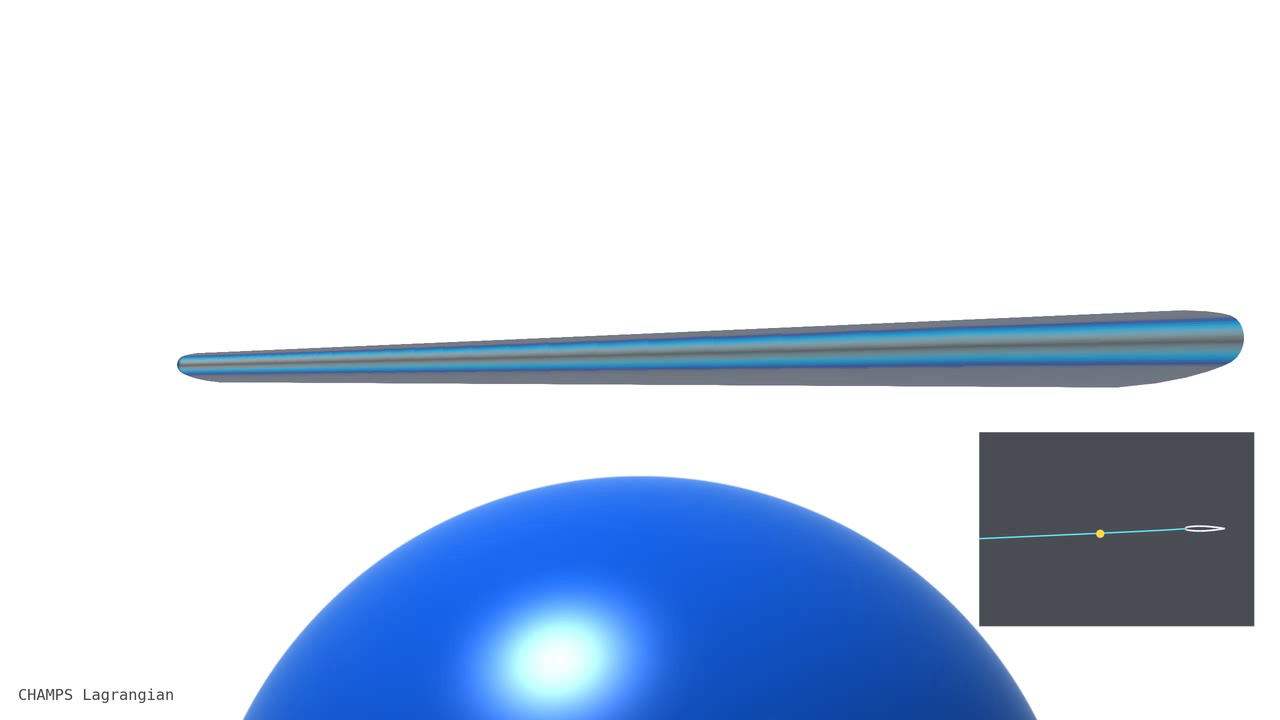
\includegraphics[width=\linewidth]{FIGURES/INTRODUCTION/DROPLET_POV_poster.png}}%
    {FIGURES/INTRODUCTION/DROPLET_POV.mp4}}%
  %{\tiny\itshape\color{gray}POV: You're a supercooled water droplet approaching an aircraft wing.\\No water droplet was harmed making the video.\par}}%
\only<2>{%
  {\scriptsize\color{champsBlue}\bfseries Direct surface-node displacement}\par\vspace{0.05cm}
  \includegraphics[width=\linewidth,height=2.1cm,keepaspectratio]{FIGURES/INTRODUCTION/LAGRANGIAN_NODE_DISPLACEMENT}\par
  {\small$\mathbf{x}_{\mathrm{new}}=\mathbf{x}_{\mathrm{old}}+h_{\mathrm{ice}}\,\mathbf{n}$}\par\vspace{0.04cm}
  {\scriptsize\color{champsBlue}\bfseries Increasing geometric complexity}\par\vspace{0.05cm}
  \includegraphics[width=\linewidth,height=3.75cm,keepaspectratio]{FIGURES/INTRODUCTION/ENTANGLEMENT.png}}%
\only<3>{%
  {\scriptsize\color{champsBlue}\bfseries Immersed boundary}\par\vspace{0.05cm}
  {\setlength{\fboxsep}{0pt}\setlength{\fboxrule}{0.6pt}\fbox{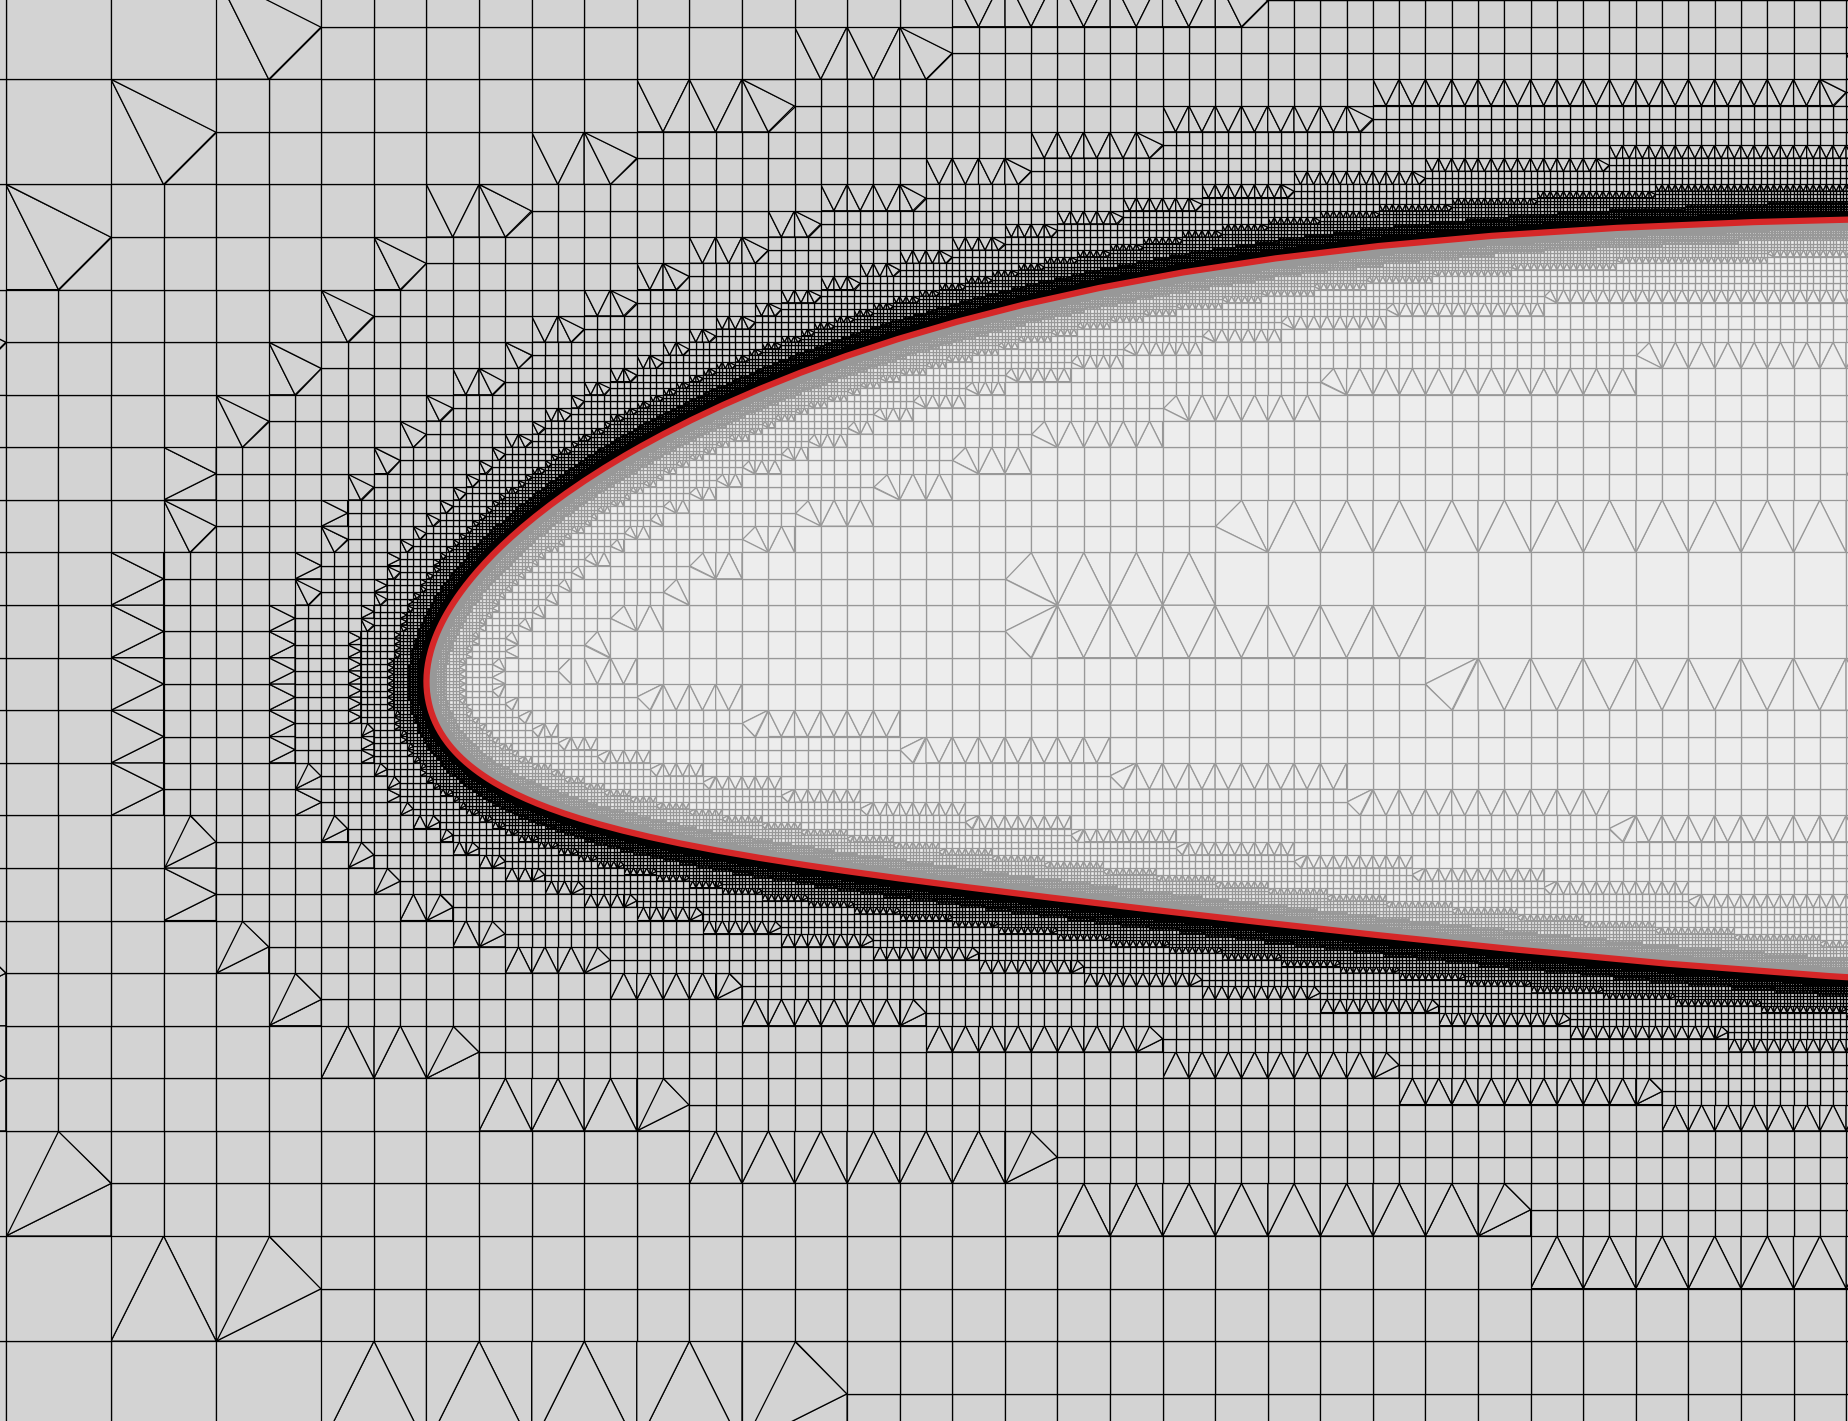
\includegraphics[width=\linewidth,height=4.5cm,keepaspectratio]{FIGURES/INTRODUCTION/meshLE_IBM}}}}%
}
\end{column}

\end{columns}

\SlideRef{lagNodeDisplacement,thompsonDeformation,lavoie2021immersed}
\end{frame}

\begin{frame}{Research Objectives}

\vspace{0.12cm}

% OVERALL OBJECTIVE
\begin{center}
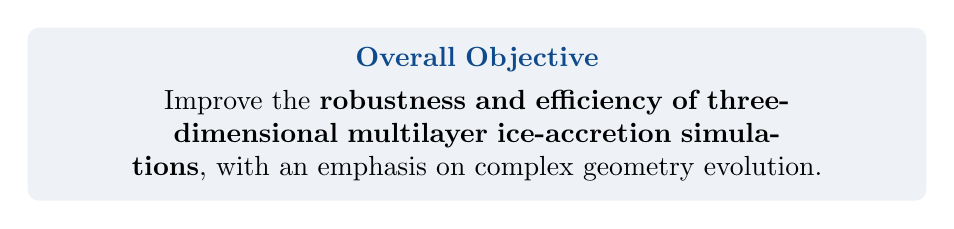
\begin{tikzpicture}
\node[
    fill=champsBlue!7,
    rounded corners=4pt,
    text width=0.90\textwidth,
    inner sep=0.25cm,
    align=center
] {
    {\color{champsBlue}\bfseries Overall Objective}\\[0.12cm]
    Improve the \textbf{robustness and efficiency of
    three-dimensional multilayer ice-accretion simulations},
    with an emphasis on complex geometry evolution.
};
\end{tikzpicture}
\end{center}

\vspace{0.30cm}

% THREE CONTRIBUTIONS
\IcingText{01 \quad Lagrangian Droplet Impingement}
{Develop efficient and scalable Lagrangian tracking
methods for complex 3D configurations,
including SLD effects.}

\par\vspace{0.28cm}

\IcingText{02 \quad Three-Dimensional Level-Set Ice Accretion}
{Develop a robust approach for multilayer
geometry evolution and surface reconstruction,
avoiding mesh entanglement.}

\par\vspace{0.28cm}

\IcingText{03 \quad Immersed Boundary Method}
{Extend the existing immersed-boundary flow solver
to enable coupled ice-accretion simulations while
reducing repeated body-fitted aerodynamic remeshing.}

\end{frame}

% Add section slides here.

%\section[Framework]{Numerical Framework}

\begin{frame}[plain]
\centering
{\Large 02\par}
\vspace{0.5cm}
{\LARGE Numerical Framework\par}
\end{frame}

% Add section slides here.

\section[LDI]{Lagrangian Droplet Impingement}

% Section transition: 03_LAGRANGIAN_DROPLET_IMPINGEMENT
{\renewcommand{\iceImgX}{1.01}\renewcommand{\iceImgY}{0.22}%
\IceSectionDivider[height=0.98\H]{}{Lagrangian\\ Droplet Impingement}{FIGURES/SECTION_TRANSITION/dropletTrajectoriesChapelCon.png}}


\begin{frame}{Droplet Impingement: Collection Efficiency}
\vspace{0.08cm}

The droplet solver determines the \textbf{local water mass flux}
reaching the aircraft surface.

\vspace{0.08cm}
\begin{columns}[T,onlytextwidth]
\begin{column}{0.43\textwidth}
{\color{champsBlue}\bfseries Collection Efficiency}

\vspace{0.04cm}
\small
The ratio of local impinging water flux to the
freestream water flux:\par\vspace{0.05cm}
{\centering$\displaystyle\beta = \frac{\dot m_{\mathrm{imp}}}{\mathrm{LWC}\,U_\infty}$\par}

\vspace{0.1cm}
{\color{champsBlue}\bfseries Water Mass Flux}\par
Accounting for the cloud liquid water content
(LWC, in g/m$^3$):\par\vspace{0.05cm}
{\centering$\boxed{\dot m_{\mathrm{imp}}=\beta\,\mathrm{LWC}\,U_\infty}$\par}
\end{column}

\begin{column}{0.54\textwidth}
\centering
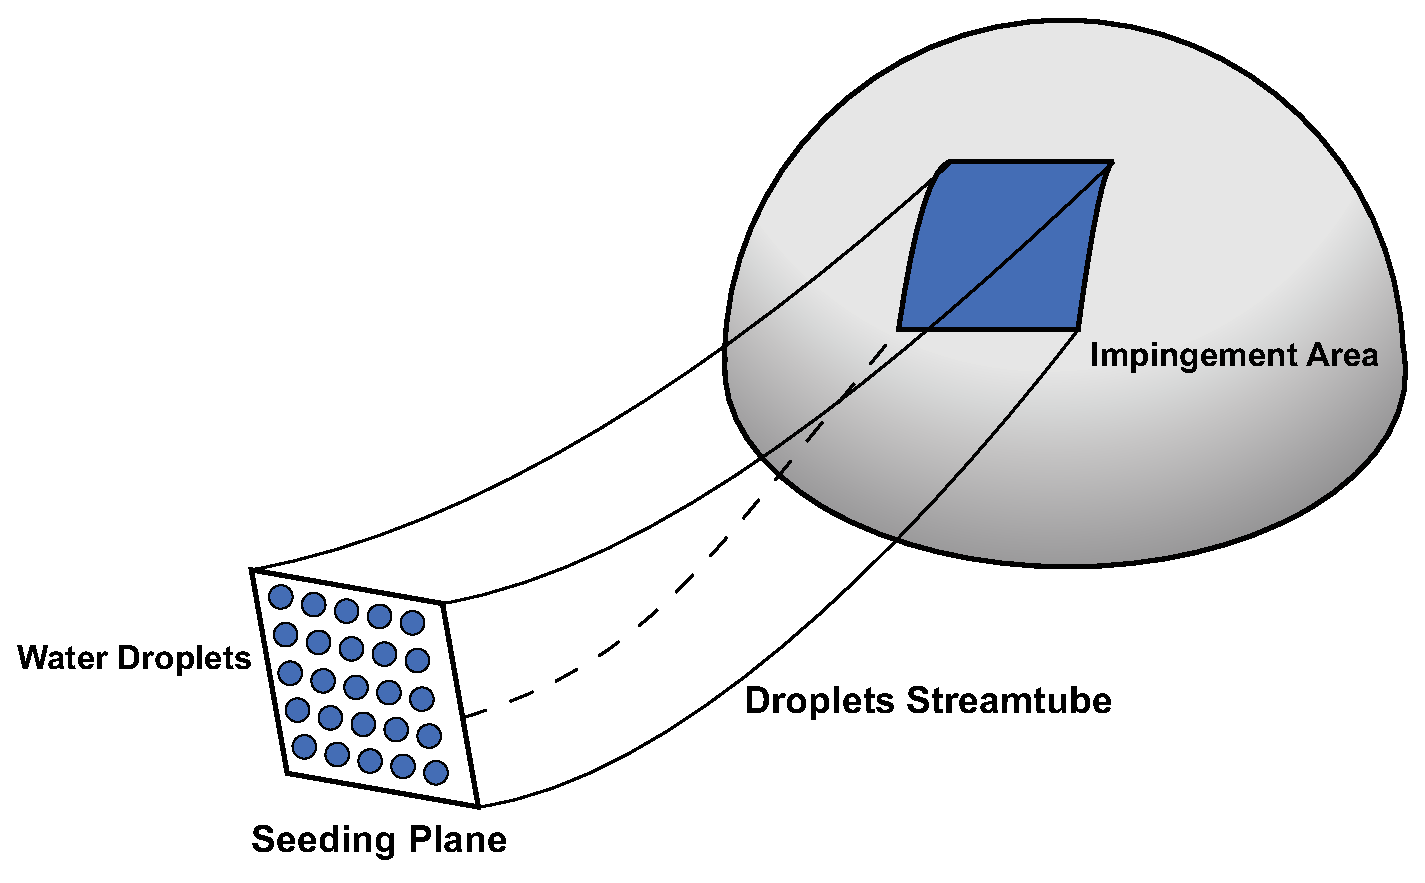
\includegraphics[
    width=\linewidth,
    height=0.43\textheight,
    keepaspectratio
]{FIGURES/LAGRANGIAN/DROP_STREAM_TUBE}

\vspace{0.05cm}
{\small
$\displaystyle\beta = \frac{A_\infty}{A_{\mathrm{imp}}}$
}
\end{column}
\end{columns}

\vspace{0.04cm}
{\color{champsBlue}\bfseries Droplet-Size Distribution}\par
\vspace{0.03cm}
{\small
Either a single \textbf{Mean Volume Diameter (MVD)} or a \textbf{distribution} of bins simulated sequentially and weighted by their fraction of the total LWC.\par}

\vfill
\begin{center}

\begin{tikzpicture}
\node[fill=champsBlue!5, draw=champsBlue!18, rounded corners=4pt,
      text width=0.90\textwidth, inner sep=3pt, align=center, font=\small] {%
  \textbf{Output to thermodynamics:}
  $\dot m_{\mathrm{imp}}$ on the exposed aircraft surface.};
\end{tikzpicture}
\end{center}
\SlideRef{bourgault1999finite,bellosta2023lagrangian}
\end{frame}

\begin{frame}{Air--Droplet Coupling and Droplet Inertia}

\vspace{0.05cm}

\begin{columns}[T,onlytextwidth]

% LEFT COLUMN
\begin{column}{0.48\textwidth}

{\color{champsBlue}\bfseries
One-Way Coupling}

\vspace{0.22cm}

Typical icing conditions:

\[
\mathrm{LWC} \approx 1\ \mathrm{g/m^3},
\qquad
\frac{\mathrm{LWC}}{\rho_w}
\approx 10^{-6}
\]

\vspace{0.12cm}

{\small
The low liquid-water concentration
allows us to neglect droplet feedback
on the airflow.
}

\vspace{0.15cm}

\begin{center}
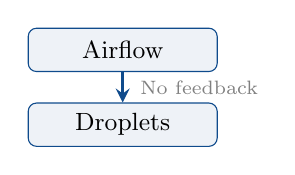
\begin{tikzpicture}[
    every node/.style={font=\small}
]

\node[
    draw=champsBlue,
    fill=champsBlue!7,
    rounded corners=3pt,
    minimum width=2.4cm,
    minimum height=0.55cm
] (air) at (0,0) {Airflow};

\node[
    draw=champsBlue,
    fill=champsBlue!7,
    rounded corners=3pt,
    minimum width=2.4cm,
    minimum height=0.55cm
] (drop) at (0,-0.95) {Droplets};

\draw[
    ->,
    >=stealth,
    champsBlue,
    very thick
] (air) -- (drop);

\node[
    right,
    font=\scriptsize,
    text=gray
] at (0.1,-0.475) {No feedback};

\end{tikzpicture}
\end{center}

\end{column}

% RIGHT COLUMN
\begin{column}{0.48\textwidth}

{\color{champsBlue}\bfseries
Droplet Inertia: Stokes Number}

\vspace{0.22cm}

\[
St = \frac{\tau_d}{\tau_f}
= \frac{\rho_d D^2 U_\infty}
{18\mu_a c_{\mathrm{ref}}}
\]

\vspace{0.25cm}

{\color{champsBlue}\bfseries
$St \ll 1$}

{\small
Droplets rapidly adapt to changes in
the airflow and closely follow streamlines.
}

\vspace{0.28cm}

{\color{champsBlue}\bfseries
$St \gg 1$}

{\small
Droplet inertia becomes dominant,
leading to greater deviations
from airflow streamlines.
}

\end{column}

\end{columns}

\vfill

\begin{center}

\begin{tikzpicture}
\node[fill=champsBlue!5, draw=champsBlue!18, rounded corners=4pt,
      text width=0.90\textwidth, inner sep=3pt, align=center, font=\small] {%
\textbf{The aerodynamic solution drives
droplet transport, while droplet inertia
governs their response to the flow.}};
\end{tikzpicture}
\end{center}

\SlideRef{clift2005bubbles}
\end{frame}

\begin{frame}{Droplet Impingement: Lagrangian vs. Eulerian}
\vspace{-0.1cm}
\begin{columns}[T,onlytextwidth]
\begin{column}{0.48\textwidth}
\centering
{\color{champsBlue}\bfseries\large Lagrangian}\par
\vspace{0.10cm}
\parbox[c][0.46\textheight][c]{\linewidth}{\centering{\setlength{\fboxsep}{0pt}\setlength{\fboxrule}{0.6pt}\fbox{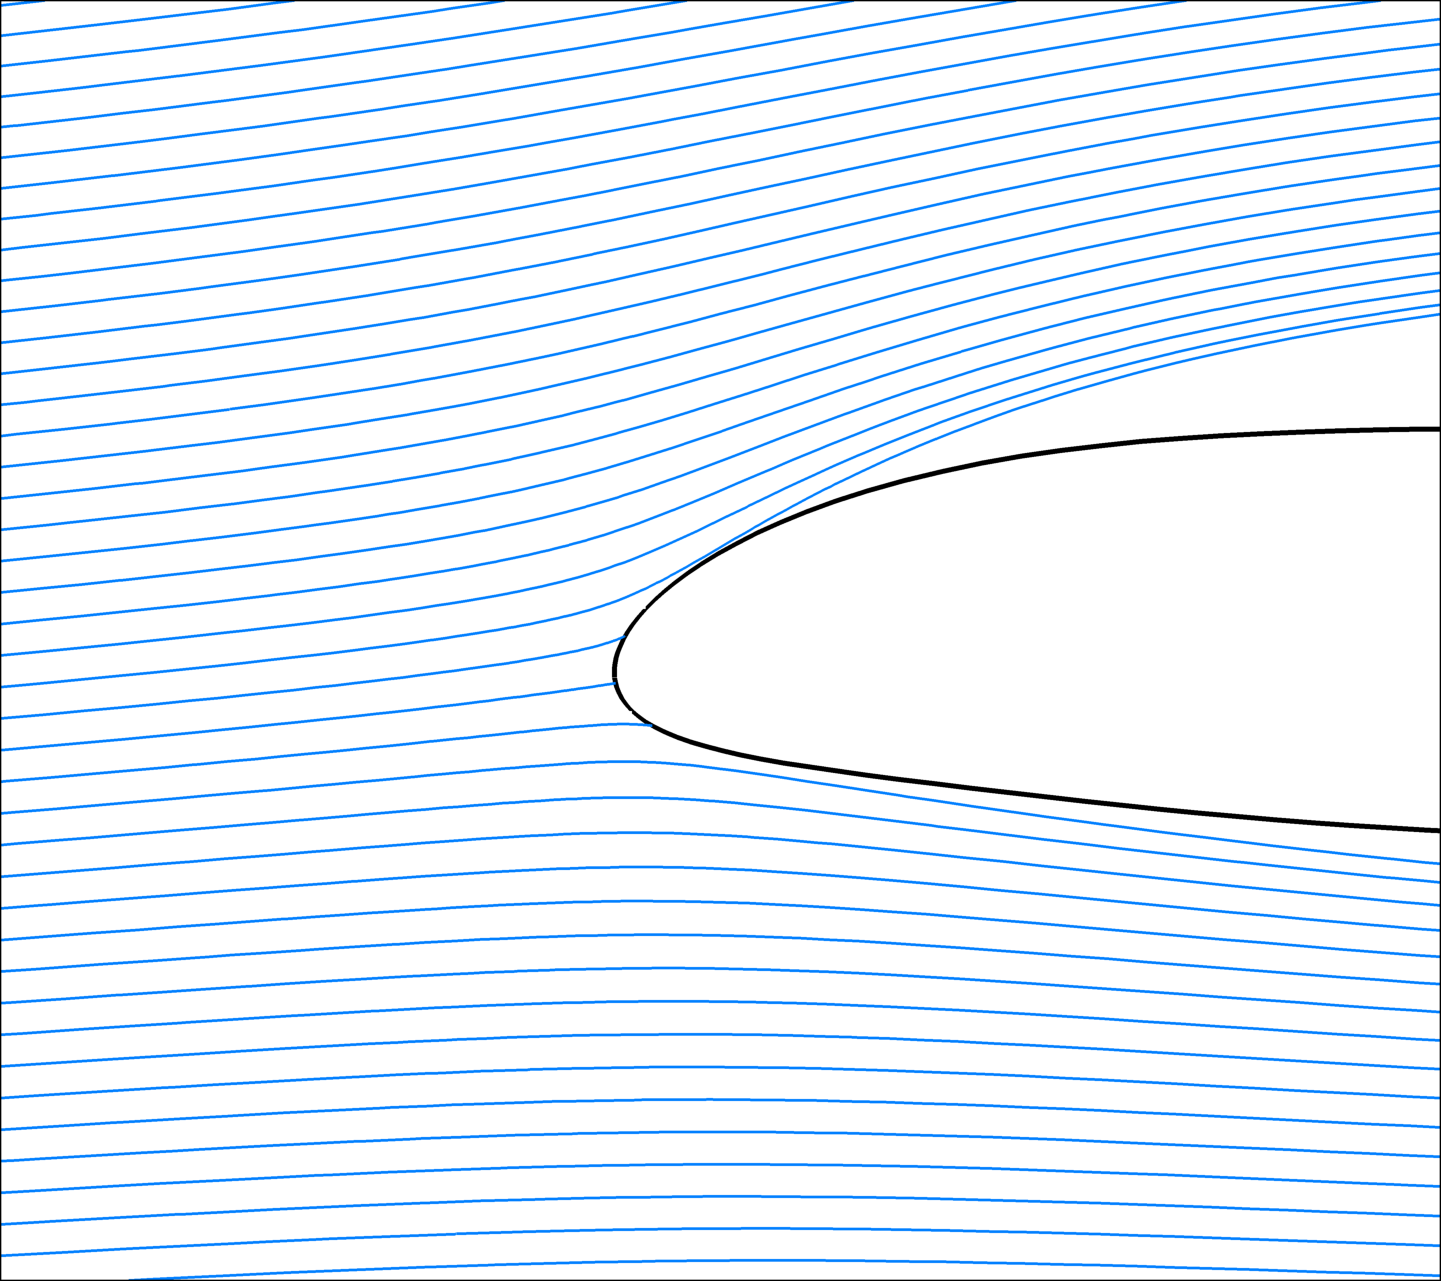
\includegraphics[width=0.96\linewidth,height=0.44\textheight,keepaspectratio]{FIGURES/LAGRANGIAN/DROP_SOLUTION.png}}}}

\vspace{0.10cm}
{\small
\textbf{Particle-based:}
$\mathbf{x}_d(t)$, $\mathbf{u}_d(t)$\par
Individual trajectories integrated through the flow.
\par}
\vspace{0.12cm}
{\scriptsize
{\color{champsBlue}\textbf{ODEs:}}\quad$\left\{\begin{aligned}
\dot{\mathbf{x}}_d&=\mathbf{u}_d\\[-1pt]
\dot{\mathbf{u}}_d&=F(\mathbf{u}_a-\mathbf{u}_d)+\mathbf{g}
\end{aligned}\right.$\par}
\end{column}

\begin{column}{0.48\textwidth}
\centering
{\color{champsBlue}\bfseries\large Eulerian}\par
\vspace{0.10cm}
\parbox[c][0.46\textheight][c]{\linewidth}{\centering{\setlength{\fboxsep}{0pt}\setlength{\fboxrule}{0.6pt}\fbox{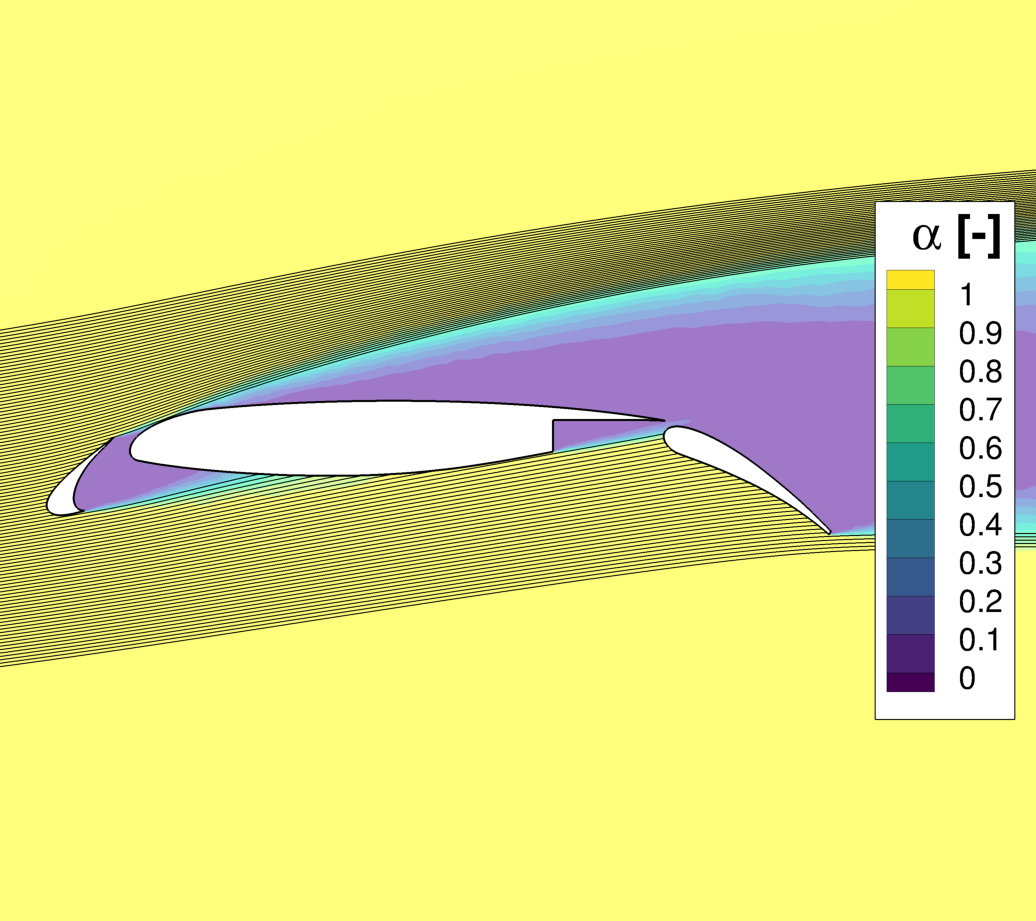
\includegraphics[
    width=0.96\linewidth,
    height=0.44\textheight,
    keepaspectratio
]{FIGURES/LAGRANGIAN/DropletVolumeFraction.png}}}}

\vspace{0.10cm}
{\small
\textbf{Field-based:}
$\alpha(\mathbf{x})$, $\mathbf{u}_d(\mathbf{x})$\par
Continuum equations on the computational mesh.
\par}
\vspace{0.12cm}
{\scriptsize
{\color{champsBlue}\textbf{PDEs:}}\quad$\left\{\begin{aligned}
\partial_t\alpha+\nabla\cdot(\alpha\mathbf{u}_d)&=0\\[-1pt]
\partial_t\mathbf{u}_d+(\mathbf{u}_d\cdot\nabla)\mathbf{u}_d&=F(\mathbf{u}_a-\mathbf{u}_d)+\mathbf{g}
\end{aligned}\right.$\par}
\end{column}
\end{columns}

\vfill
\begin{columns}[T,onlytextwidth]
\begin{column}{0.48\textwidth}
\colorbox{champsBlue!7}{%
\parbox{0.94\linewidth}{\vspace{0.09cm}\centering\scriptsize
\textbf{Advantage:} direct access to impact / SLD physics.\\[1pt]
\textbf{Trade-off:} potentially costly, irregular tracking.
\vspace{0.09cm}}}
\end{column}
\begin{column}{0.48\textwidth}
\colorbox{champsBlue!7}{%
\parbox{0.94\linewidth}{\vspace{0.09cm}\centering\scriptsize
\textbf{Advantage:} regular, scalable field solution.\\[1pt]
\textbf{Trade-off:} numerical dissipation, spurious oscillations.
\vspace{0.09cm}}}
\end{column}
\end{columns}
\SlideRef{bourgault1999finite,bellosta2023lagrangian}
\end{frame}

% ---------------------------------------------------------------------------
% Lagrangian droplet-impingement enhancements (8 slides)
% ---------------------------------------------------------------------------
\providecommand{\LDIhead}[1]{{\color{champsBlue}\bfseries #1}}
\providecommand{\LDIbottom}[1]{%
  \begin{center}%
  \begin{tikzpicture}
  \node[fill=champsBlue!5, draw=champsBlue!18, rounded corners=4pt,
        text width=0.90\textwidth, inner sep=3pt, align=center, font=\small] {#1};
  \end{tikzpicture}%
  \end{center}}

% 1 / 8 --------------------------------------------------------------
\begin{frame}[t]{Adaptive Seeding: Focusing on Impacting Droplets}
\vspace{0.05cm}
Instead of releasing a uniformly dense droplet cloud, concentrate trajectories
where they contribute to surface impingement.
\vspace{0.15cm}
\begin{columns}[T,onlytextwidth]
  \begin{column}{0.485\textwidth}
    \centering
    \LDIhead{Optional: Eulerian-Guided Initialization}\par
    \vspace{0.10cm}
    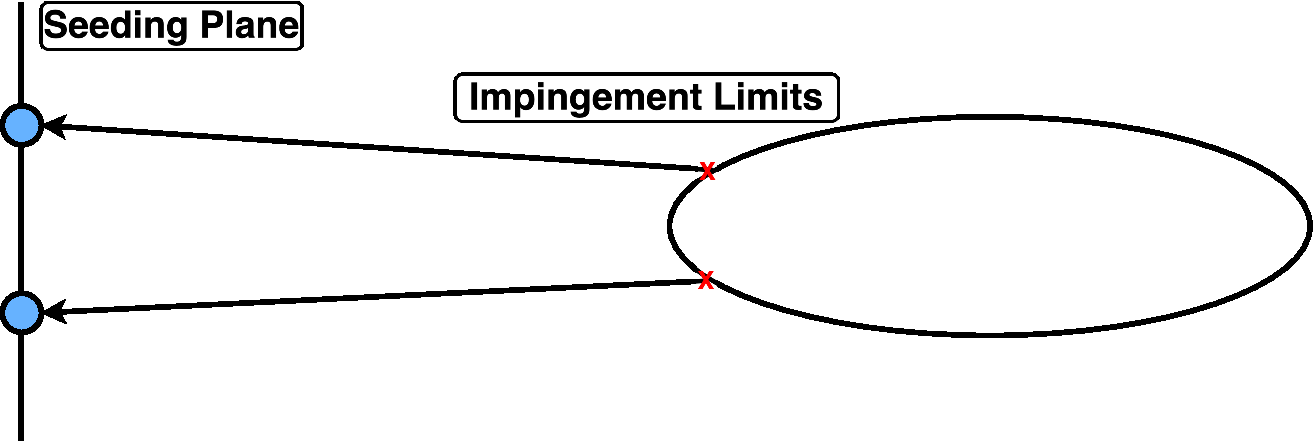
\includegraphics[width=0.97\linewidth,height=2.6cm,keepaspectratio,trim=0 0 210 0,clip]{FIGURES/LAGRANGIAN/seedingPlane-eps-converted-to.pdf}\par
    \vspace{0.02cm}
    {\small Backtrack using Eulerian droplet velocities from the surface to identify the initial upstream seeding region.\par}
  \end{column}
  \begin{column}{0.485\textwidth}
    \centering
    \LDIhead{Main Enhancement: Adaptive Refinement}\par
    \vspace{0.10cm}
    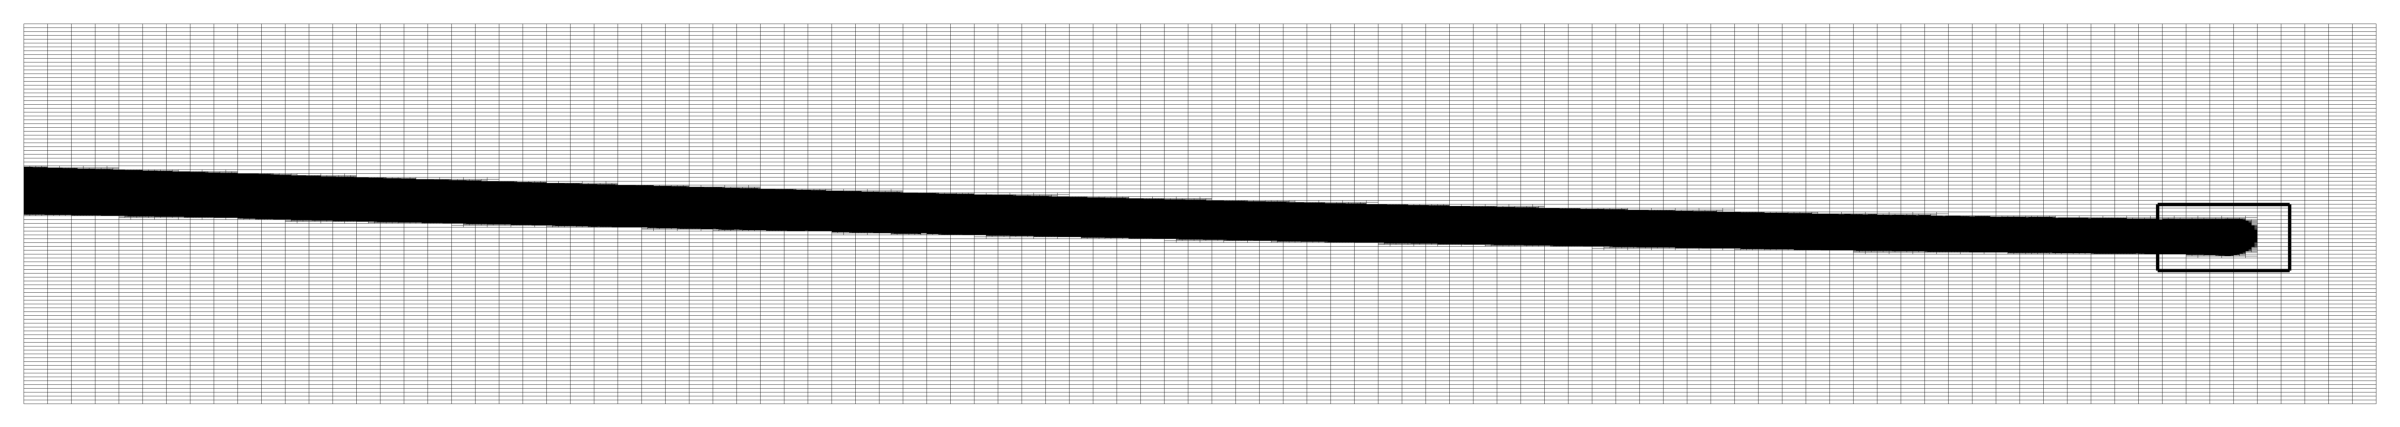
\includegraphics[width=0.97\linewidth]{FIGURES/LAGRANGIAN/seeding_grid_overview.png}\par
    \vspace{0.06cm}
    {\setlength{\fboxsep}{0pt}\setlength{\fboxrule}{0.5pt}\fbox{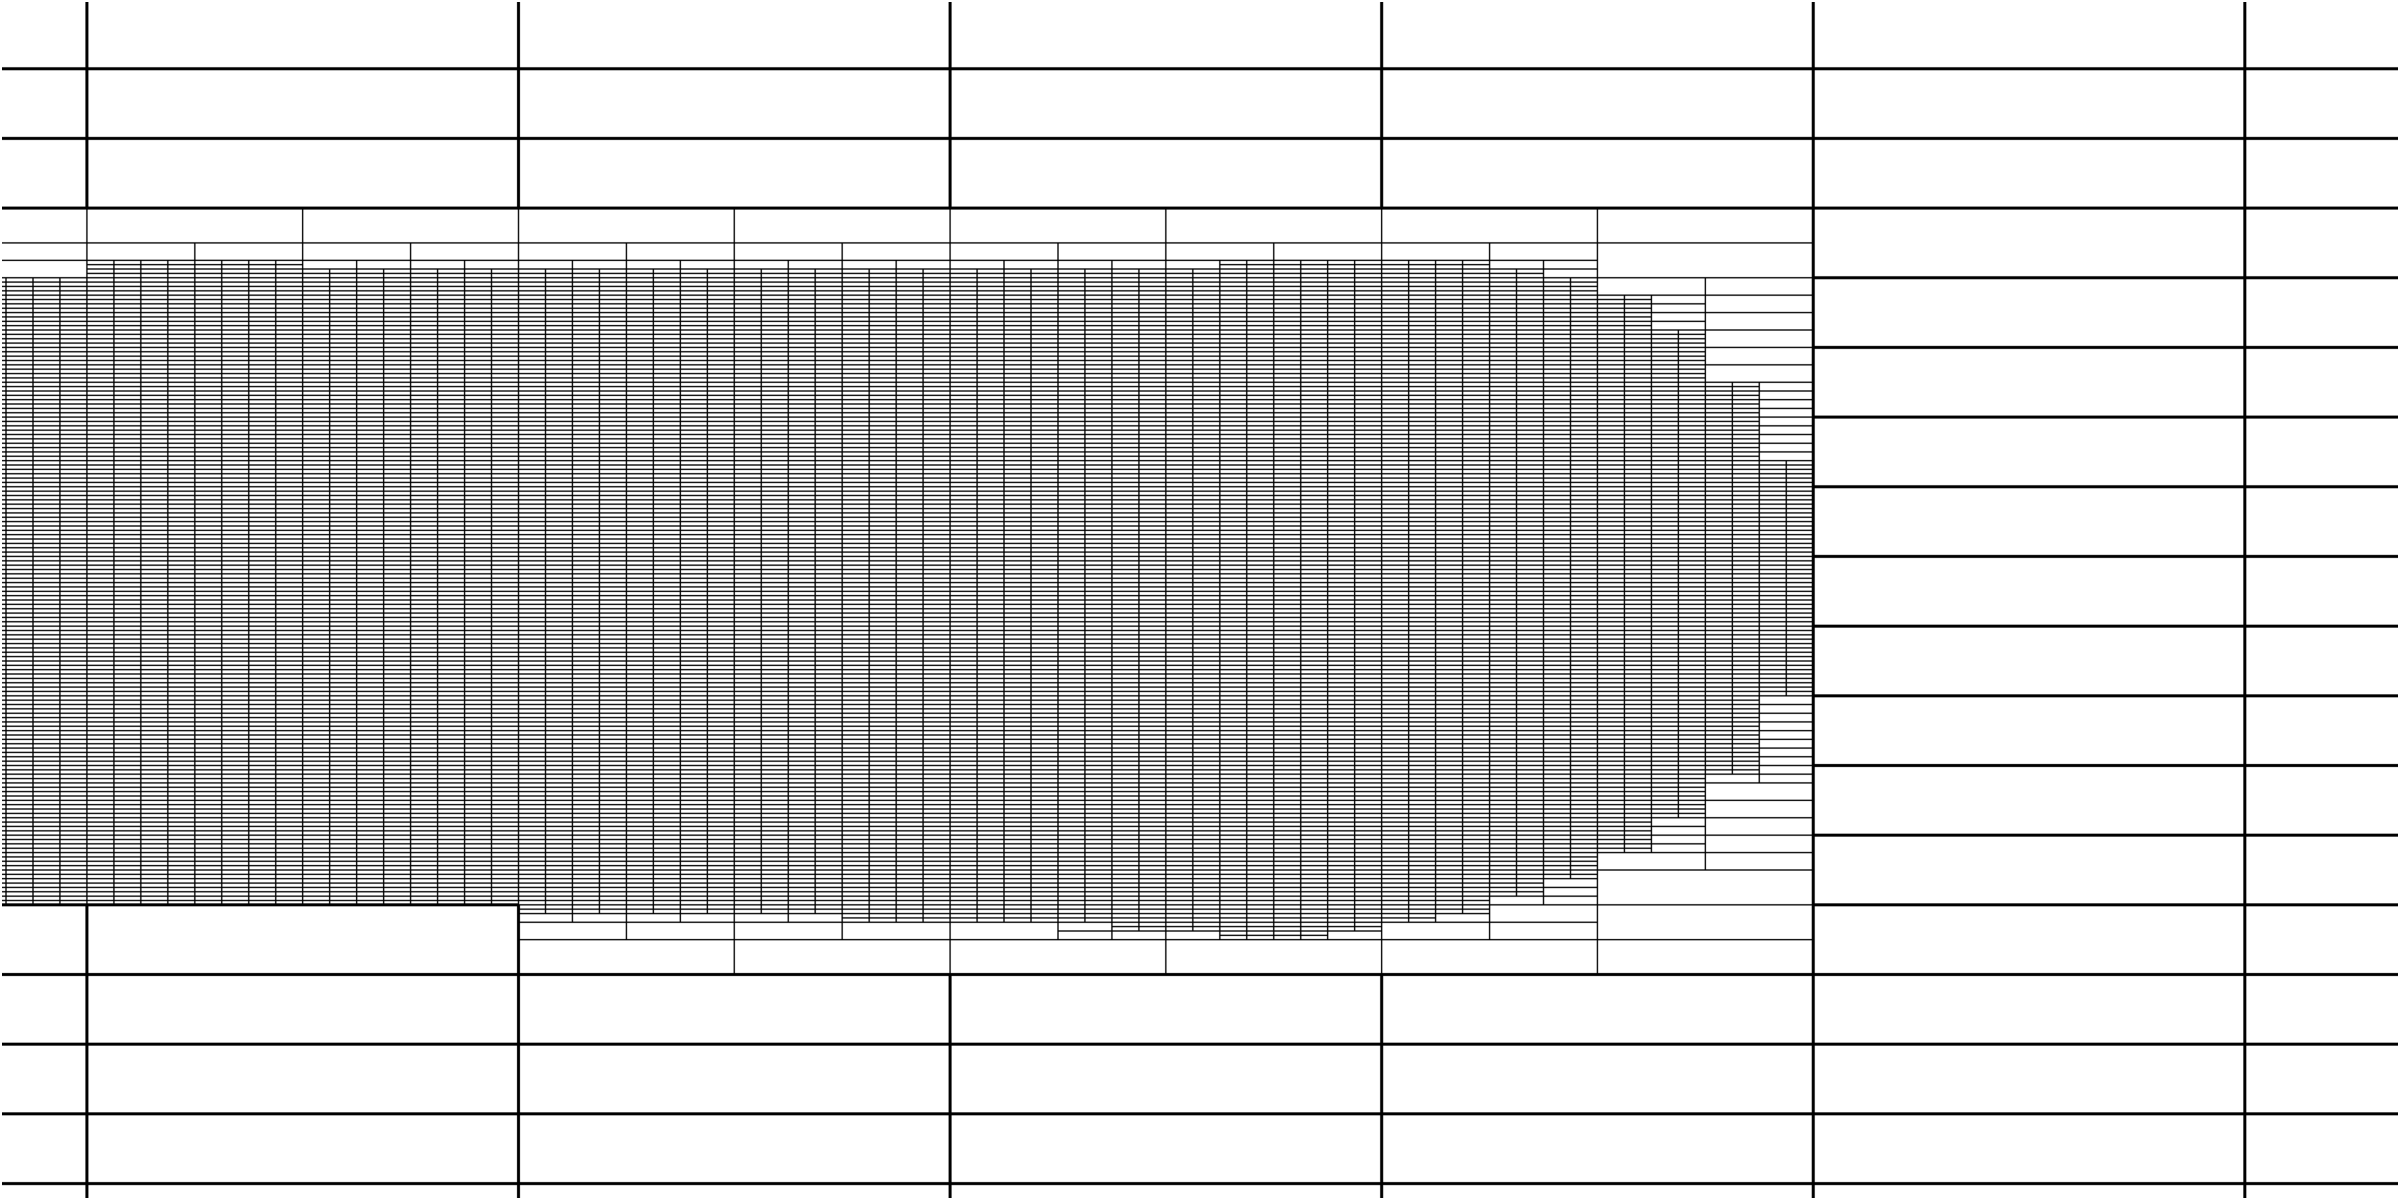
\includegraphics[height=1.55cm]{FIGURES/LAGRANGIAN/seeding_grid_zoom.png}}}\par
    \vspace{0.02cm}
    {\small Refine seeding cells associated with impacting trajectories; reuse previously computed droplets.\par}
  \end{column}
\end{columns}
\vfill
\LDIbottom{\textbf{Goal:} converged collection efficiency with far fewer unnecessary trajectories.\\[2pt]\textbf{Example:} from 10k to 262k seeding nodes (vs.\ 2.5M uniform): \textcolor{green!50!black}{\textbf{$\approx$90\% fewer droplets}}}
\SlideRef{ZAYNI2026112019}
\end{frame}

% 2 / 8 --------------------------------------------------------------
\begin{frame}{Adaptive Seeding: Convergence-Driven Refinement}
\LDIhead{Global Convergence}\par
\vspace{0.15cm}
\begin{itemize}\setlength\itemsep{0.12cm}
  \item Generate and track a coarse initial cloud.
  \item Refine only seeding cells linked to surface impacts.
  \item Monitor change in \textbf{integrated collection efficiency} between refinement passes.
  \item Stop once the prescribed global tolerance is reached.
\end{itemize}
\vspace{0.25cm}
\textbf{Stopping criterion} (successive passes $k-1$, $k$):\par
\vspace{0.25cm}
{\centering
  $\displaystyle\left|\int_S \beta^{(k)}\,dS-\int_S \beta^{(k-1)}\,dS\right| < 10^{-5}$\par}
\vspace{0.3cm}
{\color{champsBlue}Previously computed trajectories are cached and reused.}
\SlideRef{ZAYNI2026112019}
\end{frame}

% 3 / 8 --------------------------------------------------------------
\begin{frame}[t]{Face-to-Face Lagrangian Tracking}
\vspace{0.06cm}
\begin{columns}[c,onlytextwidth]
  \begin{column}{0.46\textwidth}
    \centering
    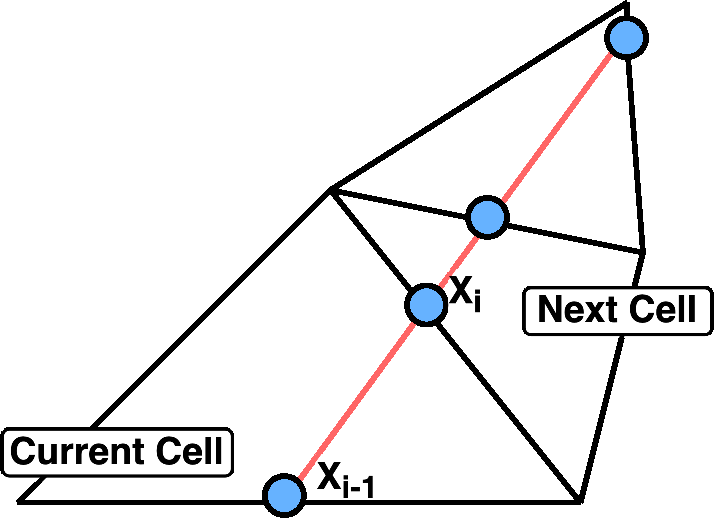
\includegraphics[width=0.99\linewidth,height=3.42cm,keepaspectratio]{FIGURES/LAGRANGIAN/Trackingface2face-eps-converted-to.pdf}\par
    \vspace{0.09cm}
    {\small Successive \textbf{ray--face intersections} identify the next cell through mesh connectivity.\par}
  \end{column}
  \begin{column}{0.51\textwidth}
    \LDIhead{Numerical Integration}\par
    \vspace{0.05cm}
    \begin{itemize}\small\setlength\itemsep{0.08cm}
      \item \textbf{Iterative BDF2} for droplet velocity.
      \item Time step set by the \textbf{local residence time inside the cell}.
      \item Droplet position localization through \textbf{facet intersections}.
      \item Direct identification of surface impact faces.
    \end{itemize}
    \vspace{0.15cm}
    {\centering
    $\boxed{\displaystyle\mathbf{u}_d^n=\frac{F\mathbf{u}_a-b\,\mathbf{u}_d^{n-1}-c\,\mathbf{u}_d^{n-2}+\mathbf{g}}{a+F}}$\par
    \vspace{0.12cm}
    {\scriptsize
    $\begin{aligned}
    a&=\frac{2\Delta t_c+\Delta t_{c-1}}{(\Delta t_c+\Delta t_{c-1})\Delta t_c}, &
    b&=-\frac{\Delta t_c+\Delta t_{c-1}}{\Delta t_c\Delta t_{c-1}},\\[0.1cm]
    c&=\frac{\Delta t_c}{(\Delta t_c+\Delta t_{c-1})\Delta t_{c-1}}, &
    F&=\frac{3C_D\rho_a\left\|\mathbf{u}_a-\mathbf{u}_d\right\|}{4\rho_d D}
    \end{aligned}$\par}
    }
  \end{column}
\end{columns}
\vfill
\SlideRef{ZAYNI2026112019,li2019fast,hairer1996}
\end{frame}

% 4 / 8 --------------------------------------------------------------
\begin{frame}[t]{Ray--Face Intersections: Triangles vs. Quadrilaterals}
\vspace{0.06cm}
\begin{columns}[c,onlytextwidth]
  \begin{column}{0.46\textwidth}
    \centering
    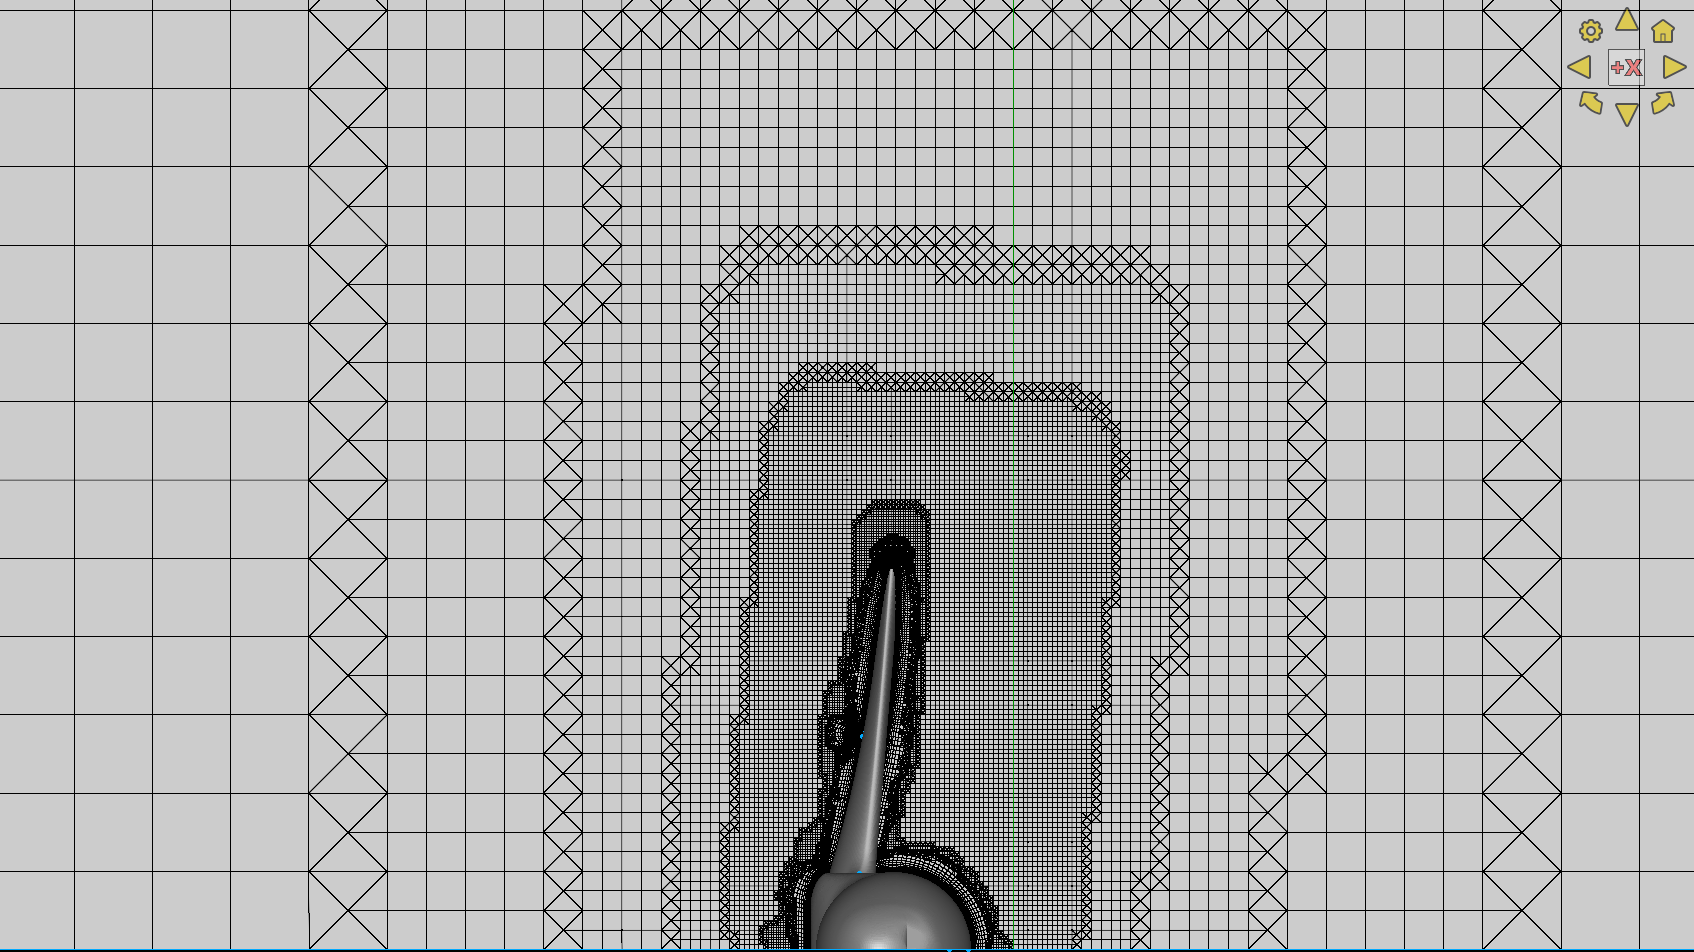
\includegraphics[width=0.99\linewidth,height=3.25cm,keepaspectratio]{FIGURES/LAGRANGIAN/CASE_2p1_MESH_CUT.png}\par
    \vspace{0.10cm}
    {\small Hexahedral-dominant CFD meshes introduce large numbers of quadrilateral faces.\par}
  \end{column}
  \begin{column}{0.51\textwidth}
    \LDIhead{Triangular Faces}\par
    \vspace{0.10cm}
    {\small Planar: standard \textbf{M\"oller--Trumbore} ray--triangle intersection.}\par
    \vspace{0.24cm}
    \LDIhead{Quadrilateral Faces}\par
    \vspace{0.12cm}
    {\small Quad vertices need not be coplanar. Two strategies:}\par
    \begin{enumerate}\setlength\itemsep{0.15cm}
      \item Split into \textbf{two triangles}: simple, but introduces an artificial diagonal.
      \item Treat the face as a \textbf{bilinear patch}: geometry represented continuously.
    \end{enumerate}
    \vspace{0.10cm}
    \[\mathbf p(u,v)=(1-v)\mathbf P_a(u)+v\mathbf P_b(u)\]
    \vspace{-0.08cm}
    {\centering\footnotesize Find \((t,u,v)\) such that \(\mathbf O+t\mathbf D=\mathbf p(u,v)\).\\[1pt]$\Rightarrow$ leads to a \textbf{quadratic equation}, solved by Ramsey et al.\par}
  \end{column}
\end{columns}
\vfill
\LDIbottom{Repeated face intersections make the ray--facet algorithm a computational bottleneck.}
\SlideRef{ZAYNI2026112019}
\end{frame}

% 5 / 8 --------------------------------------------------------------
\begin{frame}[t]{GARP: Fast Ray--Bilinear Patch Intersection}
\vspace{0.06cm}
\begin{columns}[T,onlytextwidth]
  \begin{column}{0.31\textwidth}
    \centering
    \LDIhead{1. Define Geometry}\par\vspace{0.10cm}
    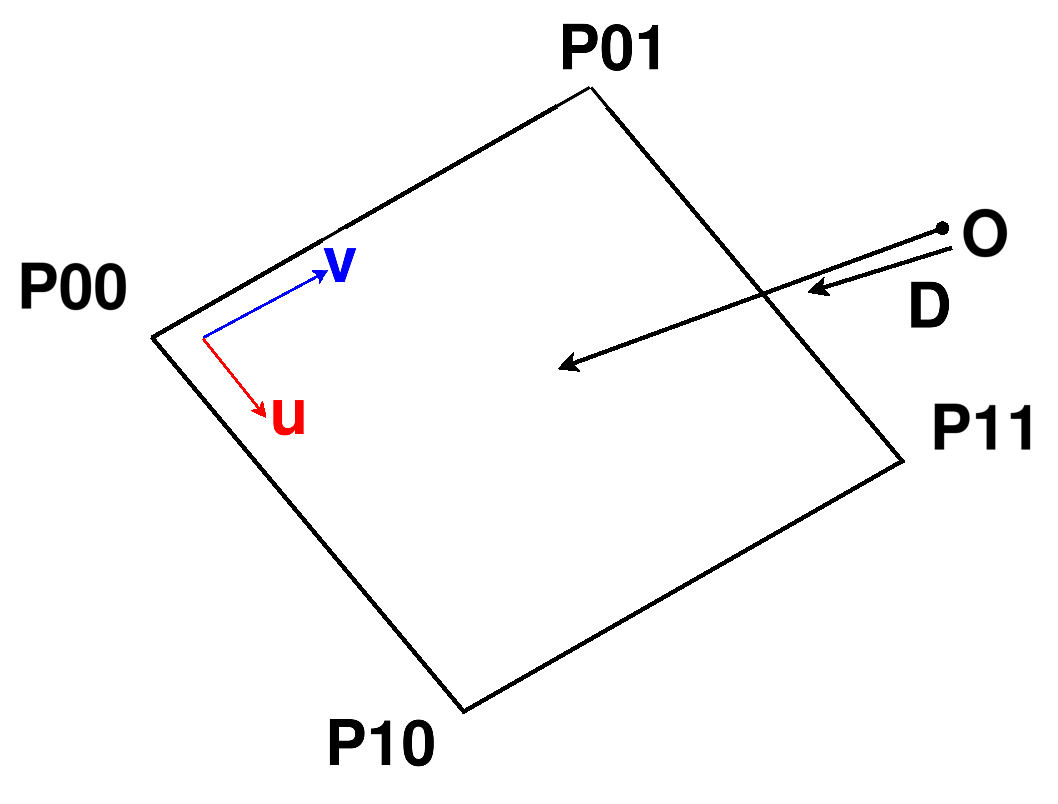
\includegraphics[width=0.98\linewidth,height=2.70cm,keepaspectratio]{FIGURES/LAGRANGIAN/GARP_STEP_0}\par
    {\scriptsize Ray and parametric bilinear patch.\par}
  \end{column}
  \begin{column}{0.31\textwidth}
    \centering
    \LDIhead{2. Determine \(u\)}\par\vspace{0.10cm}
    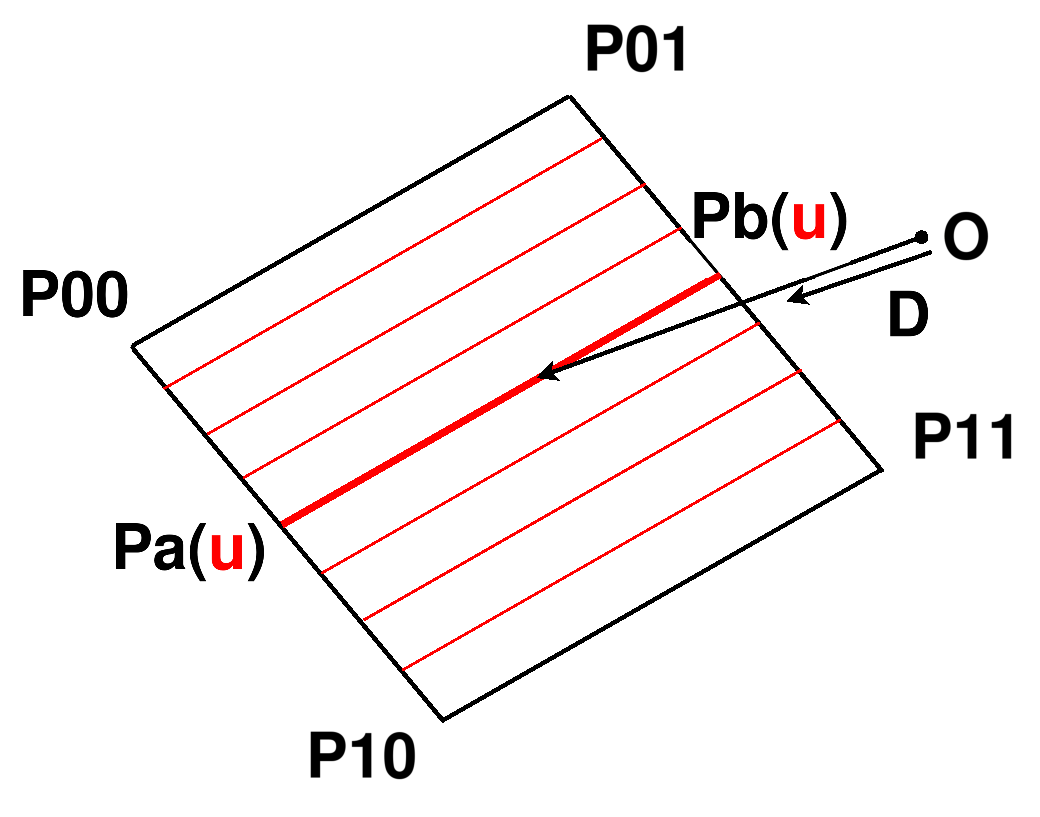
\includegraphics[width=0.98\linewidth,height=2.70cm,keepaspectratio]{FIGURES/LAGRANGIAN/GARP_STEP_1}\par
    {\scriptsize Coplanarity of a ruling segment and ray (quadratic).\par}
  \end{column}
  \begin{column}{0.31\textwidth}
    \centering
    \LDIhead{3. Determine \(v,t\)}\par\vspace{0.10cm}
    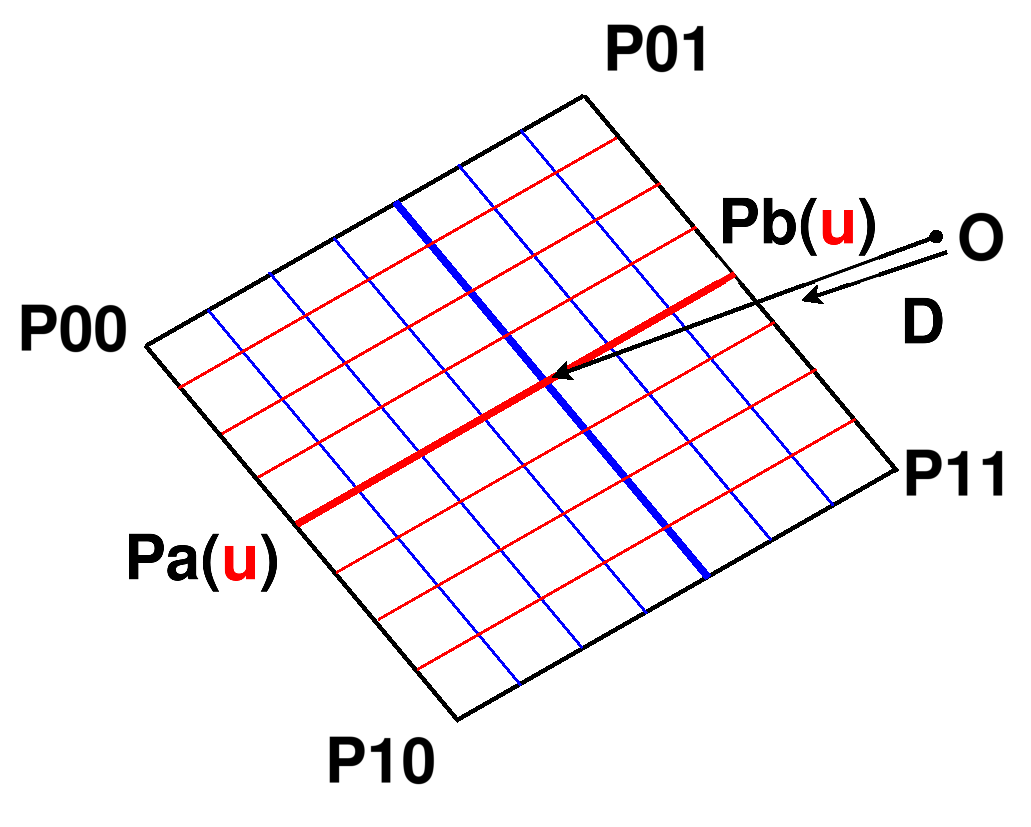
\includegraphics[width=0.98\linewidth,height=2.70cm,keepaspectratio]{FIGURES/LAGRANGIAN/GARP_STEP_2}\par
    {\scriptsize Solve ray--segment geometry; select nearest valid hit.\par}
  \end{column}
\end{columns}
\vspace{0.18cm}
\begin{center}
 {\small\color{champsBlue}\bfseries Execution-Time Reduction (1 million random ray--patch tests)}\par
 \vspace{0.09cm}
 \begin{tabular}{lcc}
  & \textbf{vs. two triangles} & \textbf{vs. Ramsey} \\
  Ramsey bilinear patch & 51.3\% & -- \\
  \rowcolor{green!18}\textbf{GARP bilinear patch} & \textbf{58.2\%} & \textbf{14.2\%} \\
 \end{tabular}
\end{center}
\SlideRef{ZAYNI2026112019}
\end{frame}

% 6 / 8 --------------------------------------------------------------
\begin{frame}[t]{Parallel Lagrangian Tracking: Data Locality and Load Balance}

\vspace{0.08cm}

{\small
Droplets are \textbf{initially distributed} among
the available computational resources.
Essential tracking data are \textbf{replicated across locales}
to minimize inter-node communication.
}

\vspace{0.05cm}

\begin{center}
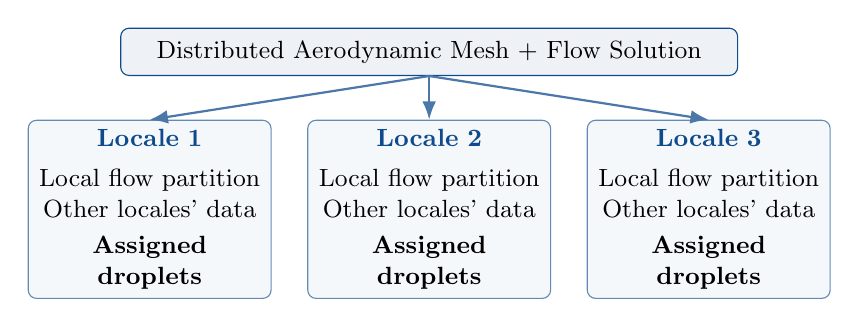
\begin{tikzpicture}[>=Latex, every node/.style={font=\small}]

% Global aerodynamic solution
\node[
    draw=champsBlue,
    fill=champsBlue!7,
    rounded corners=3pt,
    text width=7.6cm,
    align=center,
    minimum height=0.60cm
] (source) at (0,1.85)
{Distributed Aerodynamic Mesh + Flow Solution};

% Computational locales
\foreach \i/\xx in {1/-3.55,2/0,3/3.55}{

    \node[
        draw=champsBlue!65,
        fill=champsBlue!4,
        rounded corners=3pt,
        align=center,
        text width=2.85cm,
        minimum height=1.65cm
    ] (node\i) at (\xx,-0.15) {
        {\color{champsBlue}\bfseries Locale \i}\\[0.12cm]
        Local flow partition\\
        Other locales' data\\[0.08cm]
        \textbf{Assigned droplets}
    };

    \draw[->,champsBlue!75,thick]
        (source.south) -- (node\i.north);
}

\end{tikzpicture}
\end{center}

\vspace{0.02cm}

\begin{columns}[T,onlytextwidth]
  \begin{column}{0.48\textwidth}
    \LDIhead{Work Distribution}\par
    {\small \textbf{Longest Processing Time (LPT) scheduling}: assign expensive trajectories first; refine runtime estimates between adaptive seeding passes.}\par
  \end{column}
  \begin{column}{0.48\textwidth}
    \LDIhead{Data Locality}\par
    {\small Local access to flow and mesh information avoids remote reads at the cost of \textbf{increased memory usage}.}\par
  \end{column}
\end{columns}

\vfill

\SlideRef{ZAYNI2026112019,parenteau,BALDAN2023105856}

\end{frame}

% Scalability -------------------------------------------------------
\begin{frame}{Lagrangian Solver: Parallel Scalability}

\vspace{-0.05cm}

\begin{columns}[T,onlytextwidth]

% SPEEDUP
\begin{column}{0.49\textwidth}
\centering

{\color{champsBlue}\bfseries Speedup}

\vspace{0.05cm}

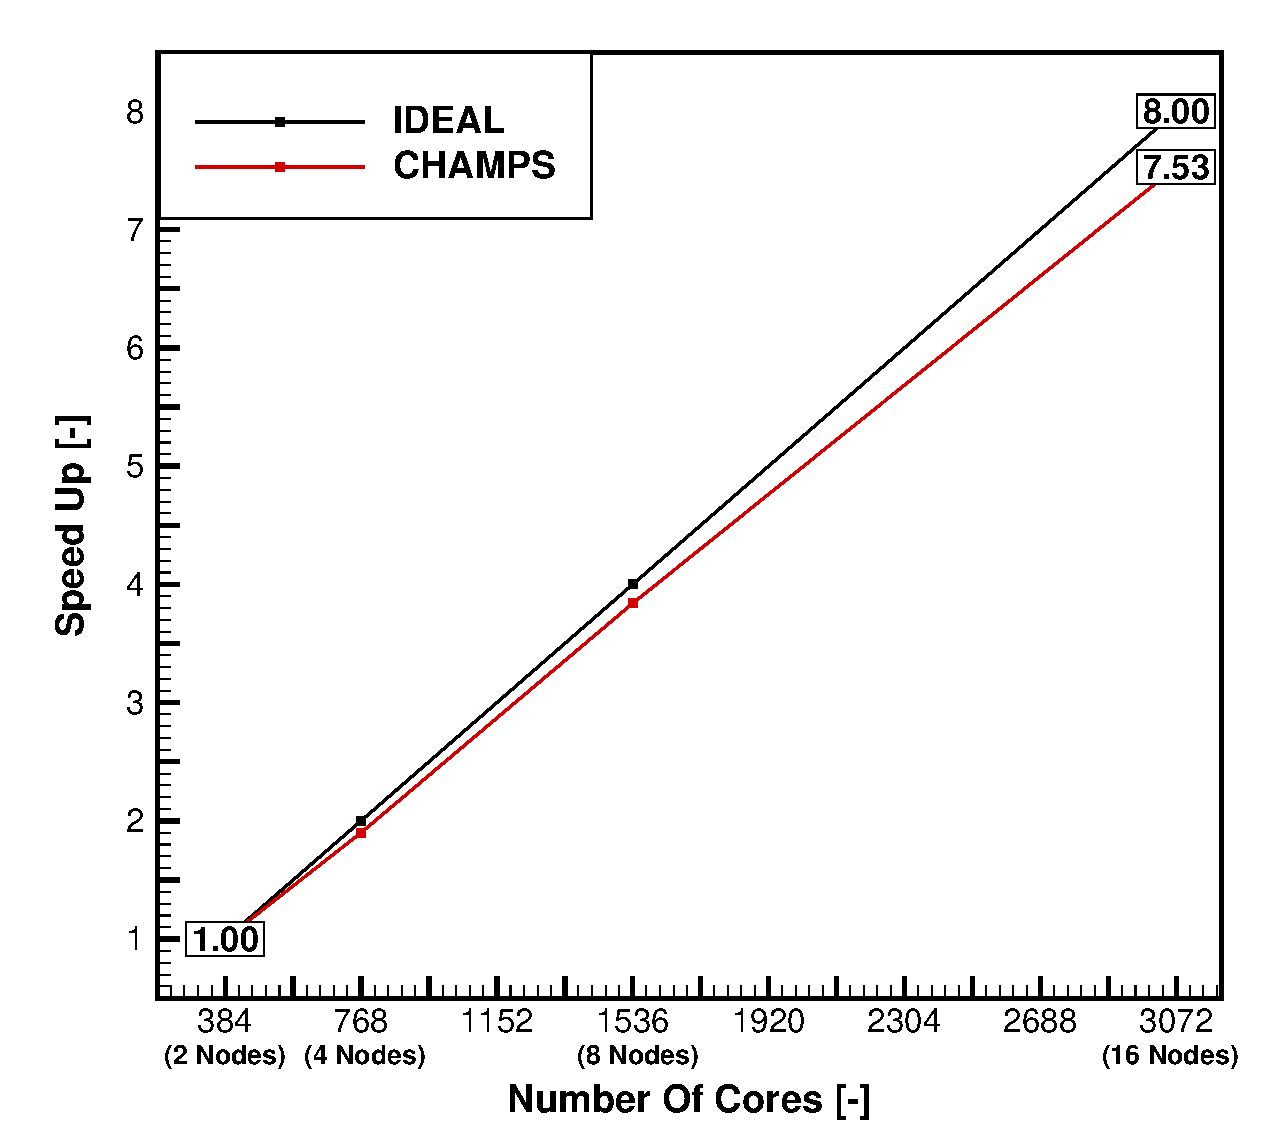
\includegraphics[
    width=\linewidth,
    height=0.56\textheight,
    keepaspectratio
]{FIGURES/LAGRANGIAN/SpeedUp}

\end{column}

% EFFICIENCY
\begin{column}{0.49\textwidth}
\centering

{\color{champsBlue}\bfseries Parallel Efficiency}

\vspace{0.05cm}

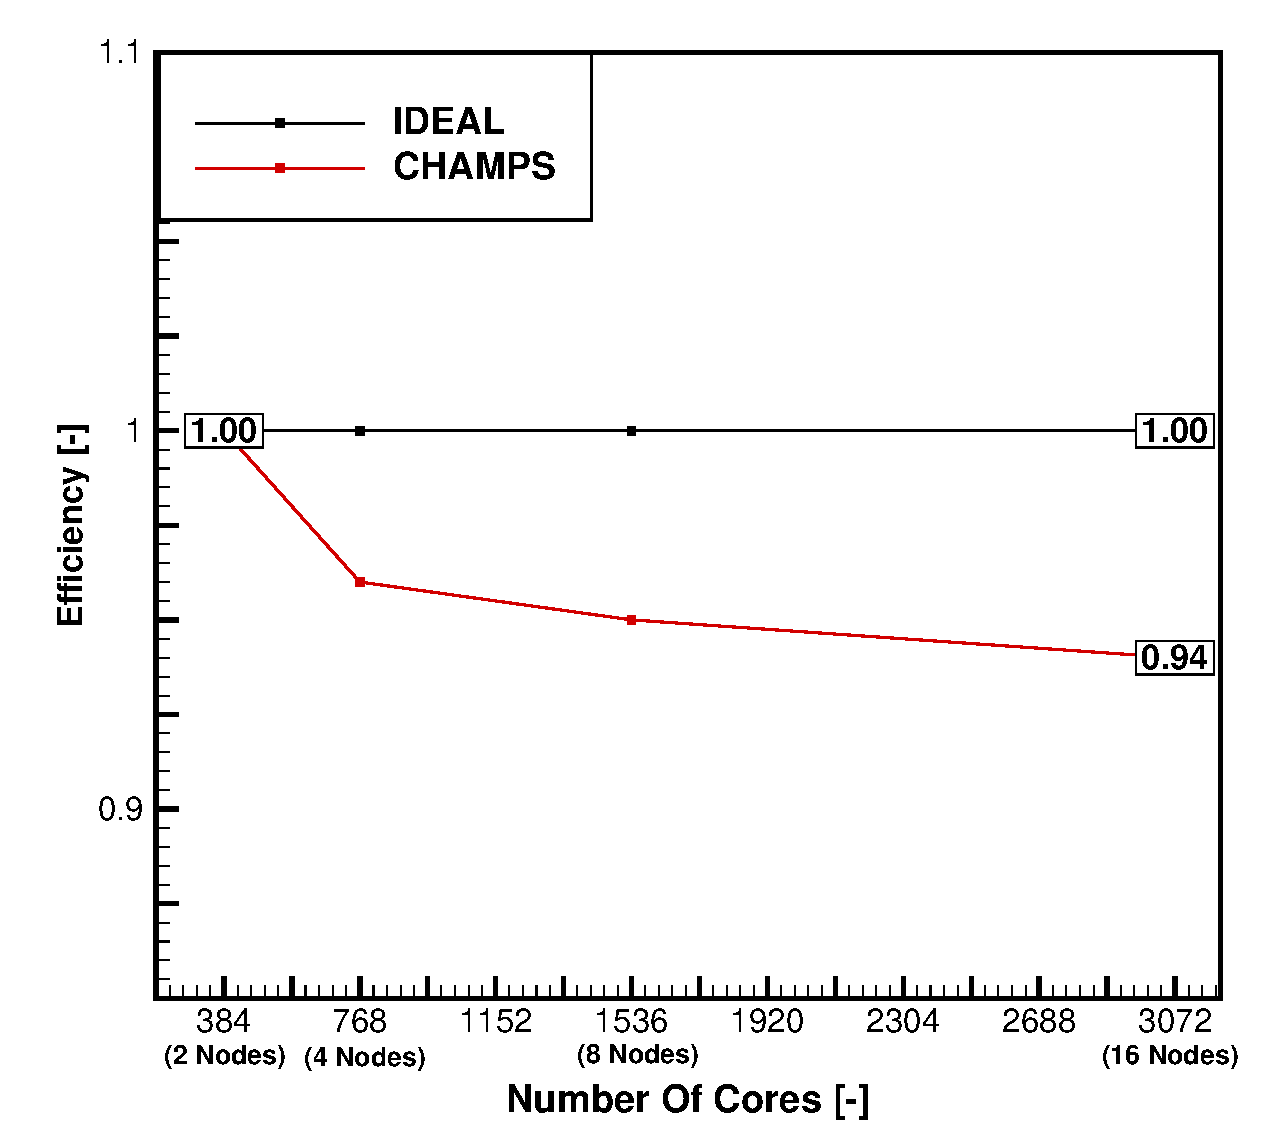
\includegraphics[
    width=\linewidth,
    height=0.56\textheight,
    keepaspectratio
]{FIGURES/LAGRANGIAN/Efficiency}

\end{column}

\end{columns}

\vspace{0.05cm}

\begin{center}
{\scriptsize
\textbf{Benchmark:} IPW2 Case 1.3
\quad $\vert$ \quad
12.8 million droplets
\quad $\vert$ \quad
384--3072 cores (2--16 nodes)\\[1pt]
\textbf{Trillium:} 2 $\times$ AMD EPYC 9655 per node (192 cores/node)
}
\end{center}

\vspace{-0.1cm}

\begin{center}
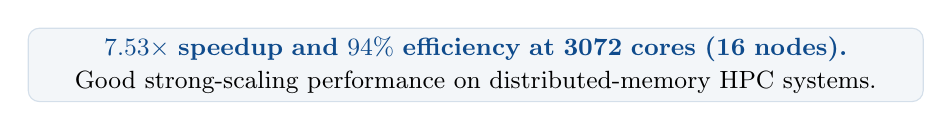
\begin{tikzpicture}
\node[fill=champsBlue!5, draw=champsBlue!18, rounded corners=4pt,
      text width=0.92\textwidth, inner sep=3pt, align=center, font=\small] {%
\textbf{\color{champsBlue}$7.53\times$ speedup and $94\%$ efficiency at 3072 cores (16 nodes).}\\[1pt]
Good strong-scaling performance on distributed-memory HPC systems.};
\end{tikzpicture}
\end{center}

\SlideRef{ZAYNI2026112019}
\end{frame}

% 7 / 8 --------------------------------------------------------------
\begin{frame}[t]{Supercooled Large Droplets: Pre-Impact and Impact Physics}
\vspace{0.04cm}
\begin{columns}[T,onlytextwidth]
  \begin{column}{0.48\textwidth}
    \centering
    \LDIhead{Pre-Impact: Deformation}\par
    \vspace{0.08cm}
    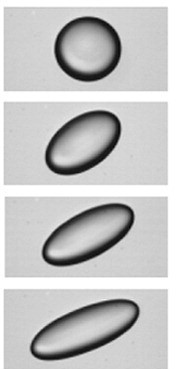
\includegraphics[width=\linewidth,height=3.9cm,keepaspectratio]{FIGURES/LAGRANGIAN/DROPLET_DEFORMATION.jpg}\par
    \vspace{0.08cm}
    {\small\textbf{Second-order effect:} changes effective drag, hence velocity and trajectory.\par}
    \vspace{0.12cm}
    \tikz\node[fill=champsBlue!7, rounded corners=4pt, inner xsep=0.3cm, inner ysep=0.12cm, font=\small]{$C_D=(1-f)C_{D,\mathrm{sphere}}+fC_{D,\mathrm{disk}}$};\par
  \end{column}
  \begin{column}{0.48\textwidth}
    \centering
    \LDIhead{At Impact: Splashing}\par
    \vspace{0.08cm}
    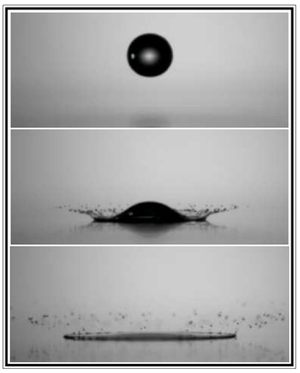
\includegraphics[width=\linewidth,height=3.9cm,keepaspectratio]{FIGURES/LAGRANGIAN/DROPLET_SPLASHING.png}\par
    \vspace{0.08cm}
    {\small\textbf{First-order effect:} a semi-empirical impact model predicts how much water is retained.\par}
    \vspace{0.12cm}
    \tikz\node[fill=champsBlue!7, rounded corners=4pt, inner xsep=0.3cm, inner ysep=0.12cm, font=\small]{$\beta_{\mathrm{retained}}=(1-f_m)\beta_0$};\par
  \end{column}
\end{columns}
\vfill
\SlideRef{wright2004semi,trontin2016revisited,honsek2006fensap}
\end{frame}

% ---------------------------------------------------------
% SLD splashing models: Wright vs ONERA
% ---------------------------------------------------------
\begin{frame}{SLD Modeling: Wright vs. ONERA}

\vspace{-0.1cm}

{\small
Semi-empirical models account for droplet splashing
and the fraction of water retained after impact.
}

\vspace{0.1cm}

\begin{columns}[T,onlytextwidth]

% WRIGHT
\begin{column}{0.48\textwidth}

{\color{champsBlue}\bfseries
Wright et al.}

\vspace{0.08cm}

{\small Mass-loss coefficient:}

{\small\vspace{-0.25cm}
\[
\begin{aligned}
f_m &= 0.7(1-\sin\theta_0)\\
&\quad\times
\left[1-\exp\left(-0.0092(K_M-200)\right)\right]
\end{aligned}
\]}

\vspace{-0.12cm}

{\scriptsize
Splashing criterion: $K_M>200$,
$\theta_0<\pi/2$, with\par\vspace{0.03cm}
{\centering$K_M=\dfrac{0.859\,K^{1/2}\left(\rho_w/\mathrm{LWC}\right)^{1/8}}{\sin^{5/4}(\theta_0)}$,\quad $K=Oh\,Re_d^{5/4}$\par}
}

\end{column}

% ONERA / TRONTIN
\begin{column}{0.48\textwidth}

{\color{champsBlue}\bfseries
ONERA -- Trontin et al.}

\vspace{0.08cm}

{\small Mass-loss coefficient:}

{\small\vspace{-0.25cm}
\[
f_m =
1-
g\left(\frac{\theta}{\theta_c}\right)
f\left(\frac{K_c-K_0}{K_0}\right)
\]}

\vspace{0.05cm}

{\scriptsize
Splashing criterion:
$K_c=We\,Oh^{-2/5}>K_0=657$.
}

\end{column}

\end{columns}

\vspace{0.08cm}

\hrule

\vspace{0.08cm}

{\color{champsBlue}\bfseries
Wright: Secondary-Droplet Reinjection}

\vspace{0.04cm}
{\centering\small
$u_{n,\mathrm{post}}=u_{n,\mathrm{imp}}\left(1.075-0.0025\,\alpha_{\mathrm{imp}}\right),\qquad
u_{t,\mathrm{post}}=u_{t,\mathrm{imp}}\left(0.300-0.0020\,\alpha_{\mathrm{imp}}\right),$\\[0.08cm]
$D_{\mathrm{new}}=D\,\exp(-0.0281K_M)$\par}

\vspace{0.04cm}

{\scriptsize
The ejected mass is represented by a secondary-droplet
parcel, tracked until domain exit or reimpingement.
}

\vfill

\LDIbottom{\textbf{Collection-efficiency correction:}
\mbox{$\beta_{\mathrm{retained}}=(1-f_m)\,\beta_0$}\\(Wright: secondary reimpingement can also be added).}
\begin{tikzpicture}[remember picture,overlay]
  \node[anchor=south west,font=\tiny,text=gray,inner sep=0pt]
      at ([xshift=0.1cm,yshift=0.27cm]current page.south west)
      {\cite{wright2004semi,trontin2016revisited}\qquad $We=\frac{\rho_w U_d^2 D}{\sigma_w},\quad Oh=\frac{\mu_w}{\sqrt{\rho_w\sigma_w D}}$};
\end{tikzpicture}
\end{frame}


% 8 / 8 --------------------------------------------------------------
\begin{frame}[t]{SLD: Secondary-Droplet Reimpingement}
\vspace{0.04cm}
\begin{columns}[c,onlytextwidth]
  \begin{column}{0.57\textwidth}
    \centering
    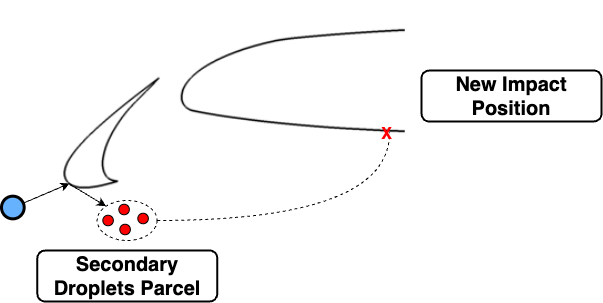
\includegraphics[width=0.99\linewidth,height=3.60cm,keepaspectratio]{FIGURES/LAGRANGIAN/dropletSplashing.png}\par
    \vspace{0.07cm}
    {\small Secondary parcels are launched from a splash event and tracked toward possible downstream impacts.\par}
  \end{column}
  \begin{column}{0.40\textwidth}
    \LDIhead{Wright-Type Splashing Model}\par
    \vspace{0.12cm}
    \begin{enumerate}\setlength\itemsep{0.16cm}
      \item Evaluate impact velocity and angle.
      \item Estimate splashed mass fraction.
      \item Inject secondary-droplet parcels.
      \item Track new trajectories and impacts.
    \end{enumerate}
  \end{column}
\end{columns}
\vfill
\begin{center}
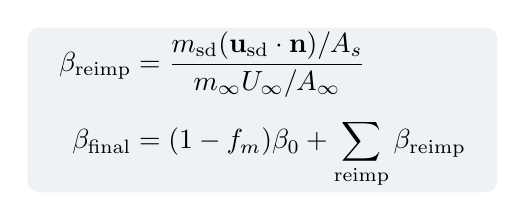
\begin{tikzpicture}
\node[fill=champsBlue!7, rounded corners=4pt, inner xsep=0.4cm, inner ysep=0.05cm]{%
$\begin{aligned}
\beta_{\mathrm{reimp}}&=\frac{m_{\mathrm{sd}}(\mathbf{u}_{\mathrm{sd}}\cdot\mathbf{n})/A_s}{m_\infty U_\infty/A_\infty}\\[0.15cm]
\beta_{\mathrm{final}}&=(1-f_m)\beta_0+\sum_{\mathrm{reimp}}\beta_{\mathrm{reimp}}
\end{aligned}$};
\end{tikzpicture}
\end{center}
\vfill
\SlideRef{wright2004semi,trontin2016revisited}
\end{frame}

% ---------------------------------------------------------------------------
% LDI results (3 slides)
% ---------------------------------------------------------------------------
% #1: geometric description, #2: Mach, #3: alpha, #4: T_inf,
% #5: Re, #6: MVD, #7: c_ref
\providecommand{\LDIResultCaseHeader}[8][]{%
\if\relax\detokenize{#1}\relax
\begin{columns}[T,onlytextwidth]
  \begin{column}{0.30\textwidth}
    {\color{champsBlue}\bfseries\scriptsize GEOMETRY}\vspace{0.05cm}
    \fcolorbox{champsBlue!24}{champsBlue!3}{%
      \parbox[c][1.17cm][c]{0.94\linewidth}{%
        \centering\scriptsize\color{champsBlue!70!black}
        Geometry figure\\[0.04cm]
        \textbf{#2}
      }%
    }
  \end{column}
  \begin{column}{0.67\textwidth}
    {\color{champsBlue}\bfseries\scriptsize CASE PARAMETERS}\par
    \vspace{0.12cm}
    {\centering\small\color{champsBlue}\bfseries
    $\bm{M_\infty=#3}$ \quad \textbf{AoA} $\bm{=#4^\circ}$ \if\relax\detokenize{#5}\relax\else\quad $T_\infty=#5$ K\fi\\[0.1cm]
    $\bm{Re=#6}$ \quad MVD $=#7\,\mu$m \quad $\bm{c_\mathrm{ref}=#8}$ m\par}
  \end{column}
\end{columns}
\else
\begin{columns}[T,onlytextwidth]
  \begin{column}{0.40\textwidth}
    {\color{champsBlue}\bfseries\scriptsize GEOMETRY}\vspace{0.05cm}
    \fcolorbox{champsBlue!24}{champsBlue!3}{%
      \parbox[c][1.0cm][c]{0.96\linewidth}{%
        \centering\scriptsize\color{champsBlue!70!black}
        \includegraphics[width=\linewidth,height=0.62cm,keepaspectratio]{#1}\\[0.04cm]
        \textbf{#2}
      }%
    }
  \end{column}
  \begin{column}{0.57\textwidth}
    {\color{champsBlue}\bfseries\scriptsize CASE PARAMETERS}\par
    \vspace{0.12cm}
    {\centering\small\color{champsBlue}\bfseries
    $\bm{M_\infty=#3}$ \quad \textbf{AoA} $\bm{=#4^\circ}$\\[0.1cm]
    $\bm{Re=#6}$ \quad MVD $=#7\,\mu$m \quad $\bm{c_\mathrm{ref}=#8}$ m\if\relax\detokenize{#5}\relax\else\quad $T_\infty=#5$ K\fi\par}
  \end{column}
\end{columns}
\fi
\vspace{0.05cm}
\endgraf
{\color{champsBlue!20}\rule{\textwidth}{0.5pt}}
\vspace{-0.1cm}
}

\providecommand{\HtailSide}{%
  {\color{champsBlue}\bfseries\scriptsize GEOMETRY}\par\vspace{0.05cm}
  \fcolorbox{champsBlue!24}{champsBlue!3}{%
    \parbox[c][1.25cm][c]{0.94\linewidth}{\centering\scriptsize\color{champsBlue!70!black}
      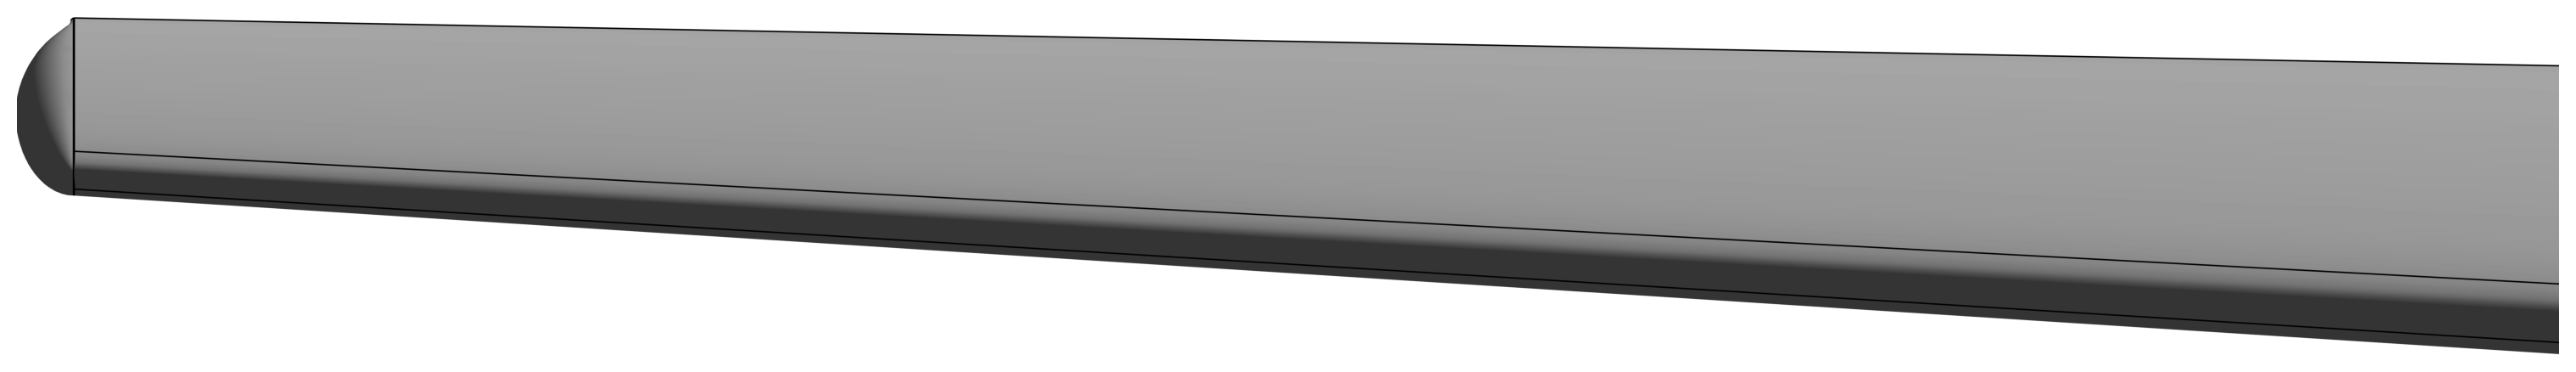
\includegraphics[width=\linewidth,height=0.85cm,keepaspectratio]{FIGURES/LAGRANGIAN/HTAIL_HORIZONTAL.png}\\[0.04cm]
      \textbf{NACA 64A008 H-tail}}}\par
  \vspace{0.3cm}
  {\color{champsBlue}\bfseries\scriptsize CASE PARAMETERS}\par\vspace{0.1cm}
  {\centering\small\color{champsBlue}\bfseries
  $\bm{M_\infty=0.23}$ \quad \textbf{AoA} $\bm{=6^\circ}$\\[0.1cm]
  $\bm{Re=5.0\times10^6}$\\[0.1cm]
  MVD $=92\,\mu$m \quad $\bm{c_\mathrm{ref}=0.956}$ m\par}}

\begin{frame}{IPW1-112: Eulerian vs. Lagrangian Results}
\begin{columns}[c,onlytextwidth]
  \begin{column}{0.33\textwidth}
    \HtailSide
  \end{column}
  \begin{column}{0.66\textwidth}\centering
    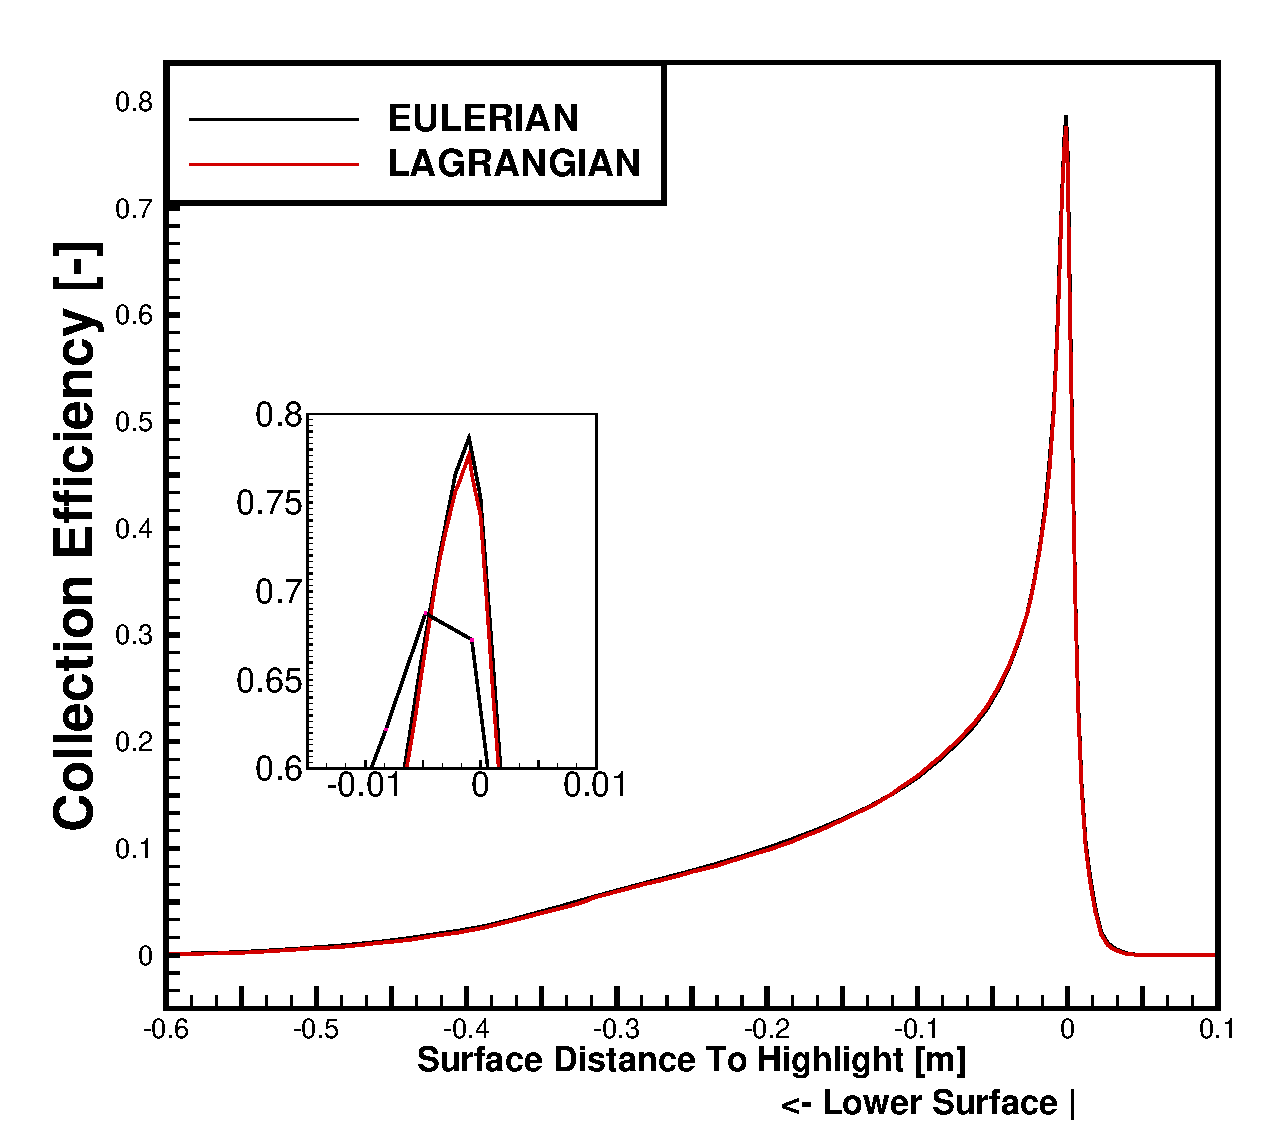
\includegraphics[width=\linewidth,height=6.3cm,keepaspectratio]{FIGURES/LAGRANGIAN/CASE_112_DISTRIBUTION}
  \end{column}
\end{columns}
\vfill
\begin{center}

\begin{tikzpicture}
\node[fill=champsBlue!5, draw=champsBlue!18, rounded corners=4pt,
      text width=0.92\textwidth, inner sep=3pt, align=center, font=\small] {%
Excellent Eulerian--Lagrangian agreement, but not yet with experiments.};
\end{tikzpicture}
\end{center}
\SlideRef{laurendeau2022summary,papadakis2007large}
\end{frame}

\begin{frame}{IPW1-112: Effect of SLD Models}
\begin{columns}[c,onlytextwidth]
  \begin{column}{0.33\textwidth}
    \HtailSide
  \end{column}
  \begin{column}{0.66\textwidth}\centering
    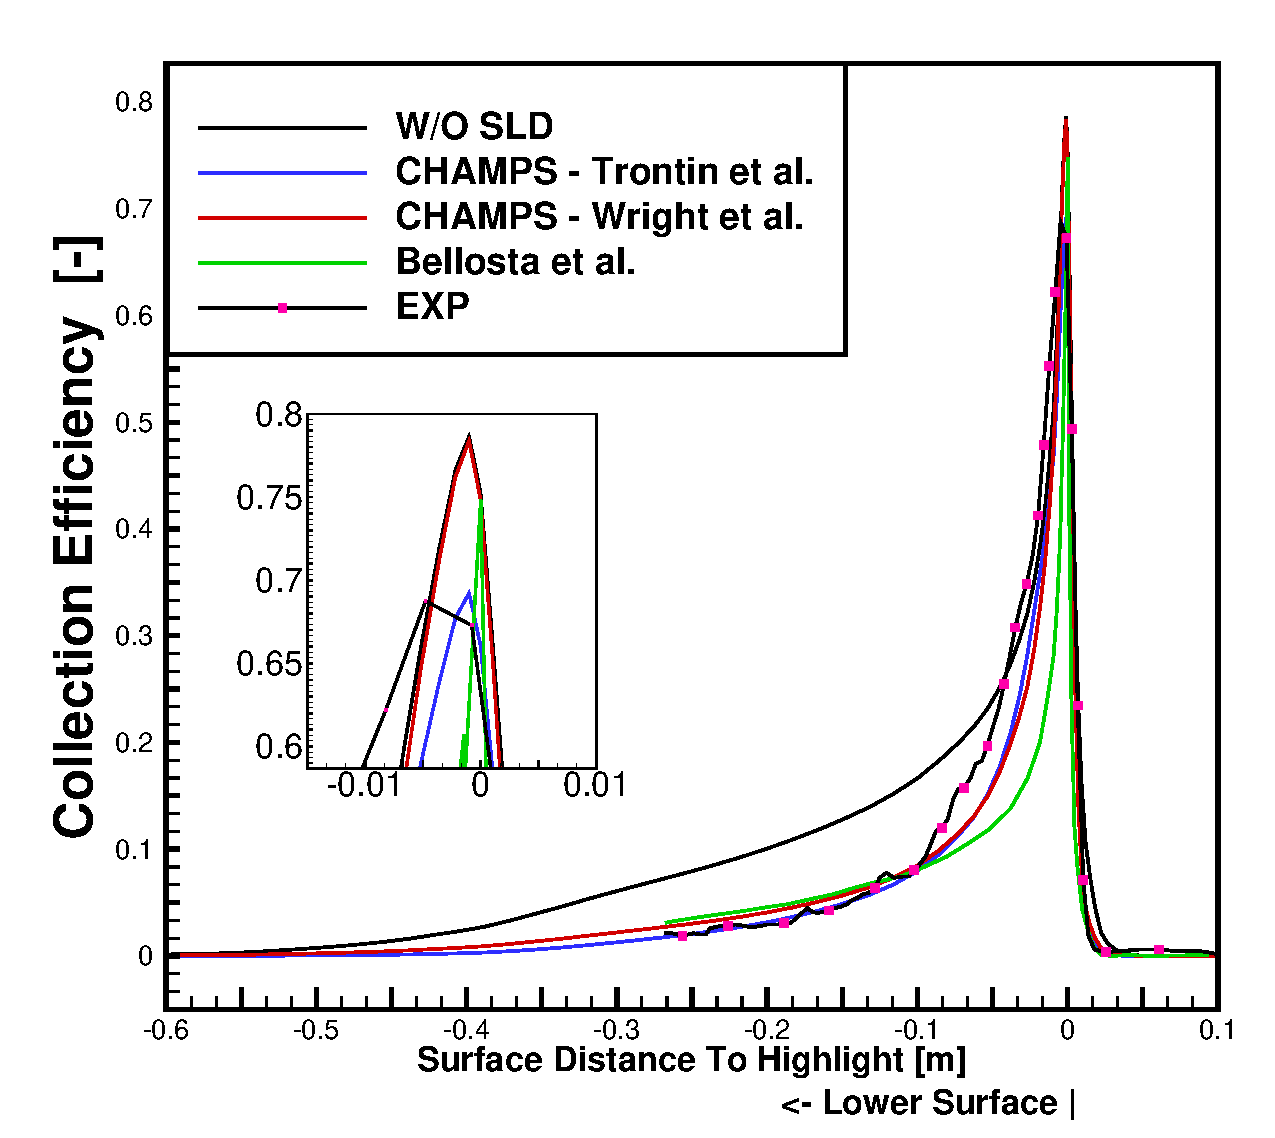
\includegraphics[width=\linewidth,height=6.3cm,keepaspectratio]{FIGURES/LAGRANGIAN/CASE_112_SLD}
  \end{column}
\end{columns}
\vfill
\begin{center}

\begin{tikzpicture}
\node[fill=champsBlue!5, draw=champsBlue!18, rounded corners=4pt,
      text width=0.92\textwidth, inner sep=3pt, align=center, font=\small] {%
SLD corrections improve agreement.};
\end{tikzpicture}
\end{center}
\SlideRef{laurendeau2022summary,papadakis2007large}
\end{frame}

\begin{frame}{IPW1-122: SLD Impingement on a Multi-Element Airfoil}
\LDIResultCaseHeader[FIGURES/LAGRANGIAN/MDA_GEOMETRY.png]{Slat / main / flap}{0.23}{4}{}{4.8\times 10^6}{92}{0.914}
\begin{columns}[T,onlytextwidth]
  \begin{column}{0.29\textwidth}
    \centering
    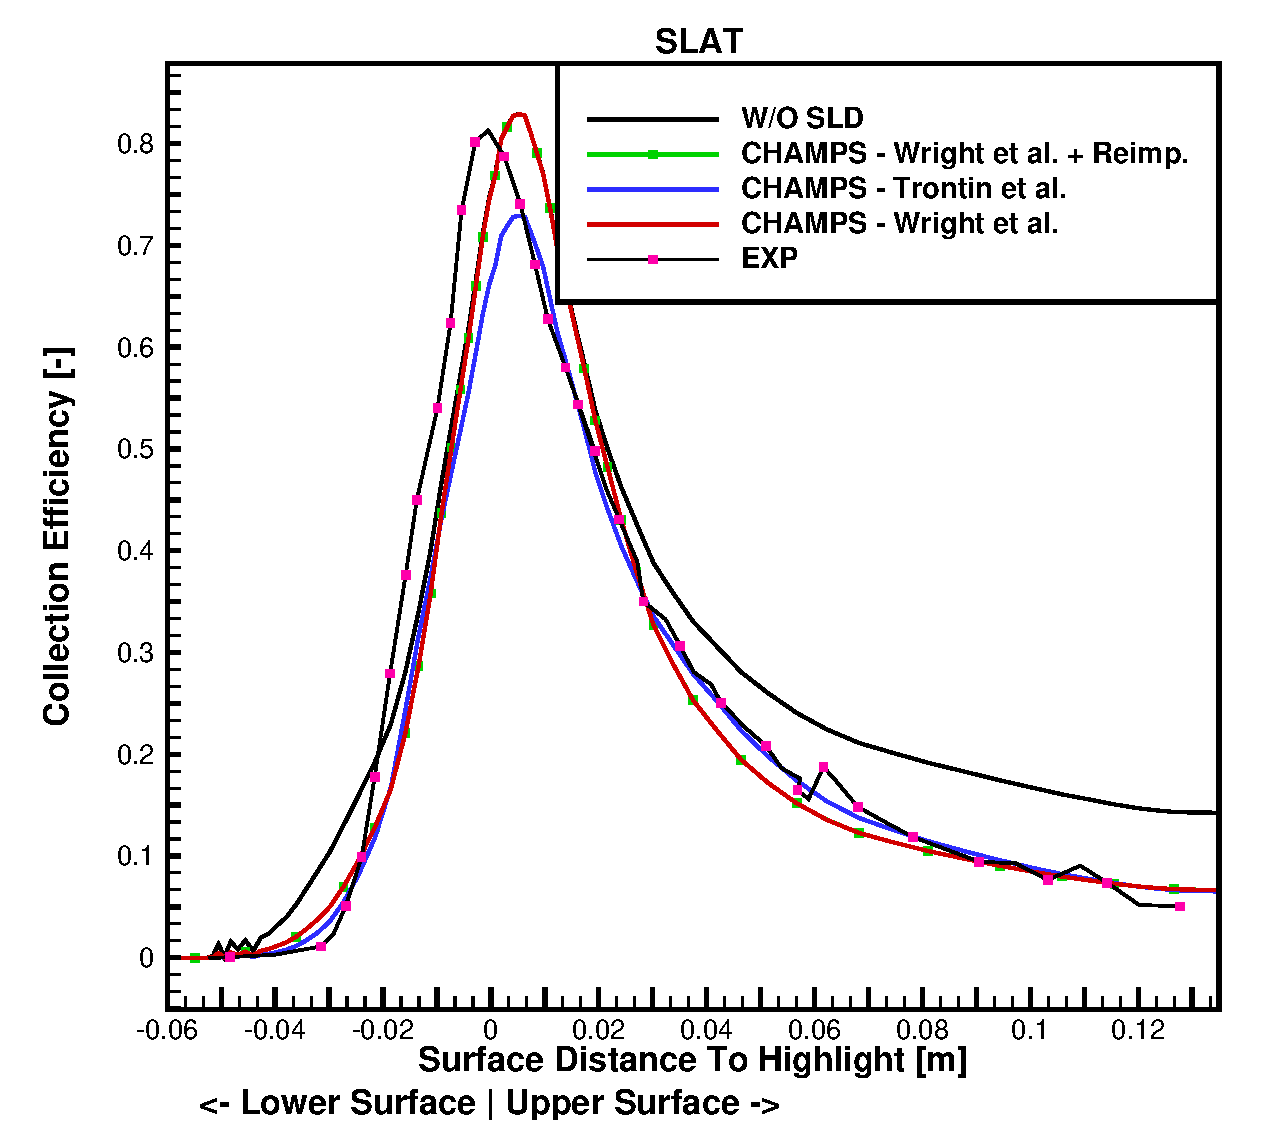
\includegraphics[width=\linewidth,height=3.3cm,keepaspectratio]{FIGURES/LAGRANGIAN/CASE_122_SLAT_SLD}\par\vspace{0.03cm}
    {\color{champsBlue}\bfseries\scriptsize SLAT}
  \end{column}
  \begin{column}{0.29\textwidth}
    \centering
    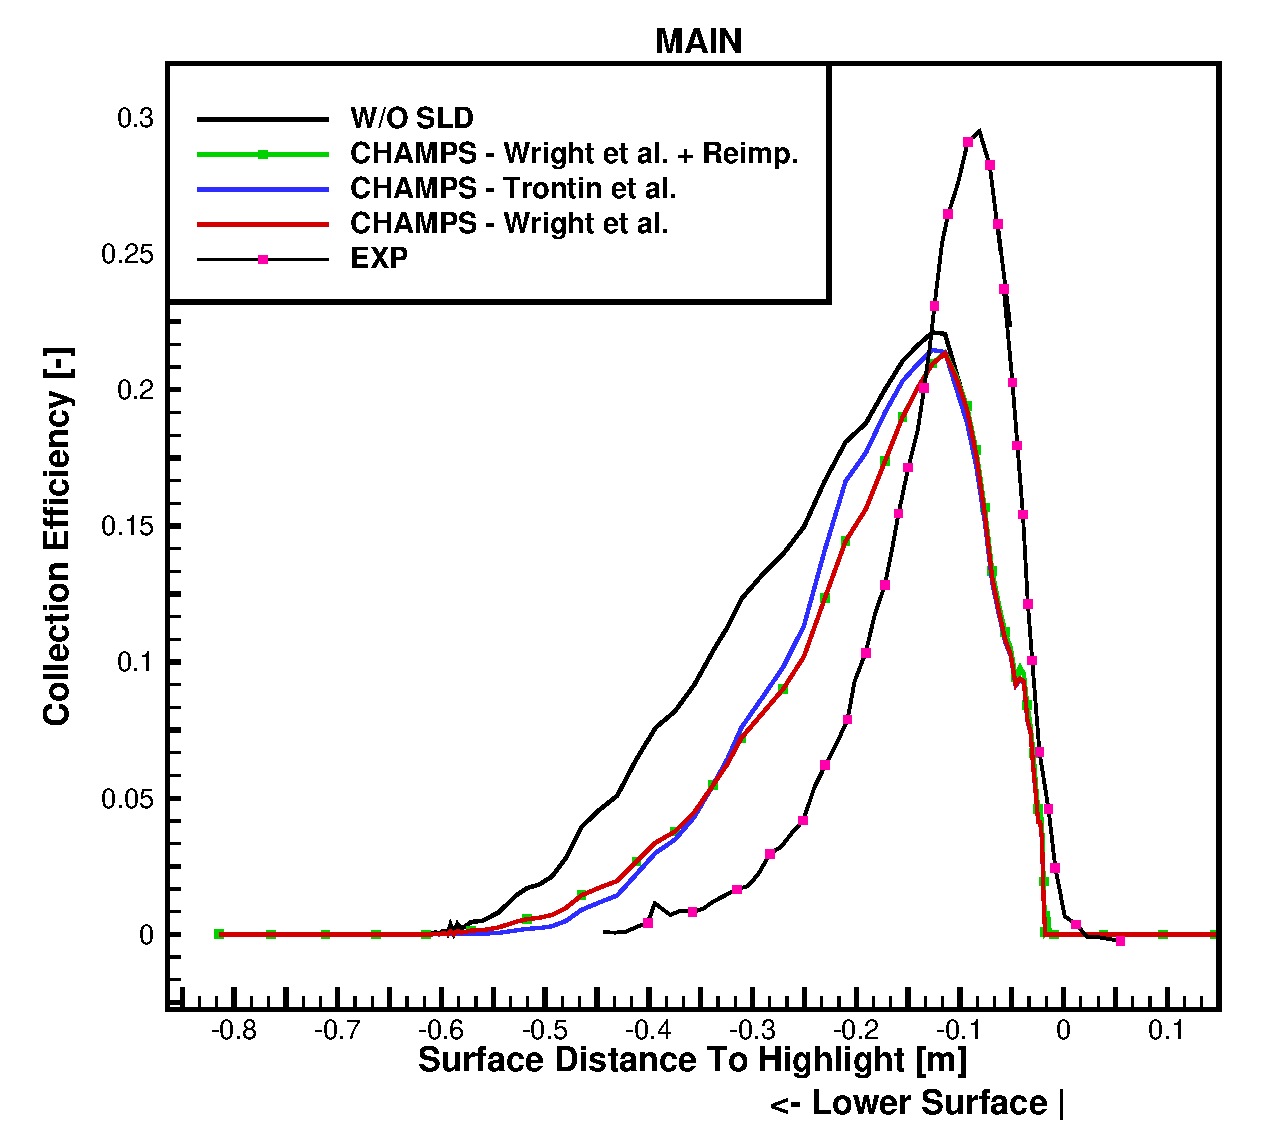
\includegraphics[width=\linewidth,height=3.3cm,keepaspectratio]{FIGURES/LAGRANGIAN/CASE_122_SLAT_MAIN}\par\vspace{0.03cm}
    {\color{champsBlue}\bfseries\scriptsize MAIN}
  \end{column}
  \begin{column}{0.29\textwidth}
    \centering
    \makebox[\linewidth][l]{\begin{tikzpicture}[spy using outlines={circle,magnification=1.9,size=1.85cm,connect spies,red,line width=0.8pt}]\node[inner sep=0,anchor=south west](im){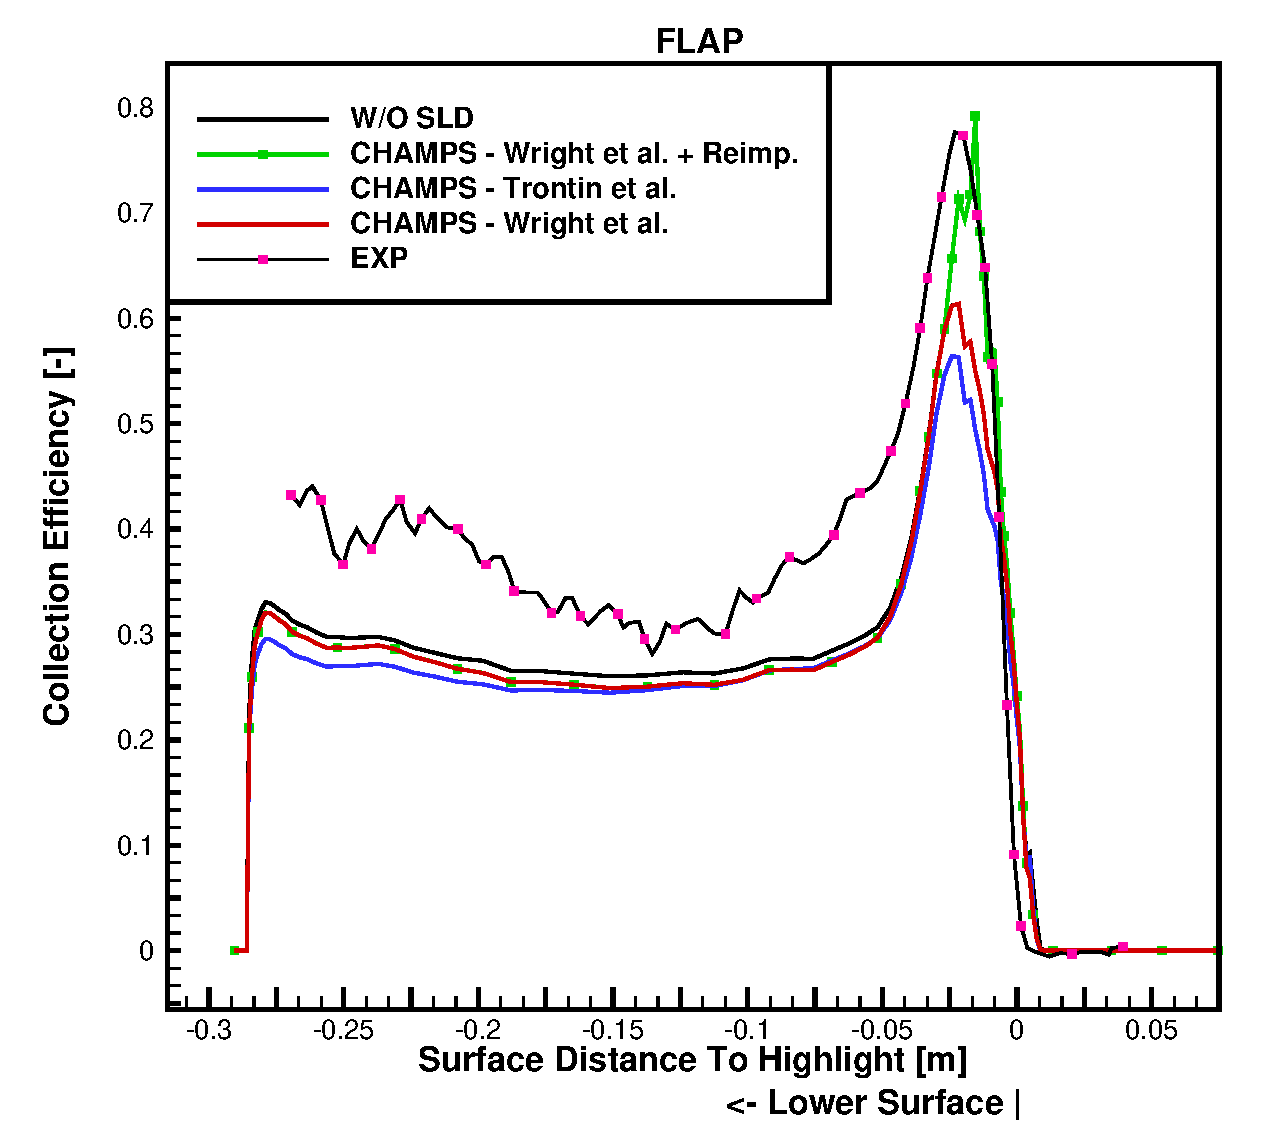
\includegraphics[width=\linewidth,height=3.3cm,keepaspectratio]{FIGURES/LAGRANGIAN/CASE_122_SLAT_FLAP}};\coordinate (pk) at ($0.772*(im.south east)+0.77*(im.north west)$);\coordinate (ln) at ($1.2*(im.south east)+0.5*(im.north west)$);\spy on (pk) in node at (ln);\end{tikzpicture}}\par\vspace{0.03cm}
    {\color{champsBlue}\bfseries\scriptsize FLAP}
  \end{column}
  \begin{column}{0.10\textwidth}\end{column}
\end{columns}
\vfill
\begin{center}
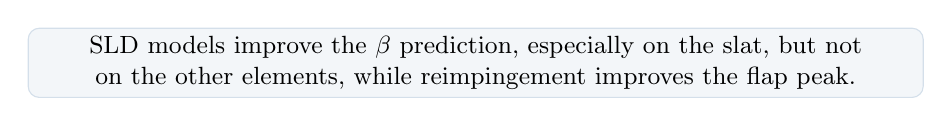
\begin{tikzpicture}
\node[fill=champsBlue!5, draw=champsBlue!18, rounded corners=4pt,
      text width=0.92\textwidth, inner sep=3pt, align=center, font=\small] {%
SLD models improve the $\beta$ prediction, especially on the slat, but not on the other elements, while reimpingement improves the flap peak.};
\end{tikzpicture}
\end{center}
\SlideRef{laurendeau2022summary}
\end{frame}

% Add section slides here.

\section[3D LS]{Three-Dimensional Level-Set Ice Accretion}

% Section transition: 04_THREE_DIMENSIONAL_LEVEL_SET_ICE_ACCRETION
{\renewcommand{\iceImgX}{1.08}%
\IceSectionDivider[trim=120 0 0 0,clip,height=1.52\H]{}{Three-Dimensional\\ Level-Set\\ Ice Accretion}{FIGURES/SECTION_TRANSITION/CLIPPED_ICE_SHAPE_CASE_362_3.png}}


% ---------------------------------------------------------------
% 1 — CONVENTIONAL LAGRANGIAN GEOMETRY EVOLUTION
% ---------------------------------------------------------------
\begin{frame}[t]{Conventional Geometry Evolution: Limitations}
\vspace{0.12cm}
\begin{columns}[T,onlytextwidth]
  \begin{column}{0.44\textwidth}
    {\color{champsBlue}\bfseries Explicit Surface Tracking}
    \vspace{0.12cm}

    \centering
    \includegraphics[width=\linewidth,height=2.05cm,keepaspectratio]{FIGURES/LEVELSET/LAGRANGIAN_NODE_DISPLACEMENT}
    \vspace{0.05cm}

    {\small
    \[
    \mathbf x_{\mathrm{new}}=\mathbf x_{\mathrm{old}}+
    h_{\mathrm{ice}}\mathbf n
    \]
    }
    \raggedright\small
    Surface nodes move along local normals, while the surrounding
    body-fitted mesh must be deformed or regenerated.
  \end{column}
  \hfill
  \begin{column}{0.53\textwidth}
    {\color{champsBlue}\bfseries Growing 3D Geometric Complexity}
    \vspace{0.10cm}

    \centering
    \includegraphics[width=\linewidth,height=3.65cm,keepaspectratio]{FIGURES/LEVELSET/ENTANGLEMENT.png}
    \vspace{0.03cm}

    {\scriptsize\color{gray}Surface-mesh distortion and entanglement near a 3D ice feature.}
    \vspace{0.08cm}

    \raggedright\small
    Horns, scallops, and concave regions may produce
    self-intersections or invalid elements.
  \end{column}
\end{columns}
\vfill
\begin{center}
  \colorbox{champsBlue!8}{\parbox{0.93\textwidth}{\centering\small
    \vspace{0.11cm}\textbf{Challenge:} Robust geometry evolution
    without preserving explicit surface-node connectivity.\vspace{0.11cm}}}
\end{center}
\end{frame}

% ---------------------------------------------------------------
% 2 — IMPLICIT SURFACE REPRESENTATION
% ---------------------------------------------------------------
\begin{frame}[t]{Implicit Interface Tracking: The Level-Set Method}
\vspace{0.12cm}
\begin{columns}[c,onlytextwidth]
  \begin{column}{0.40\textwidth}
    {\color{champsBlue}\bfseries Implicit Geometric Description}
    \vspace{0.15cm}

    \small
    The evolving ice--air boundary is represented by the
    \textbf{zero contour} of a signed-distance field $\phi$.
    \vspace{0.20cm}

    \[
    \boxed{\Gamma(t)=\{\mathbf x:\phi(\mathbf x,t)=0\}}
    \]

    \vspace{0.14cm}
    \begin{tabular}{@{}ll@{}}
      $\phi<0$ & Solid / ice\\[3pt]
      $\phi=0$ & Ice--air interface\\[3pt]
      $\phi>0$ & Air
    \end{tabular}
  \end{column}
  \hfill
  \begin{column}{0.58\textwidth}
    \centering
    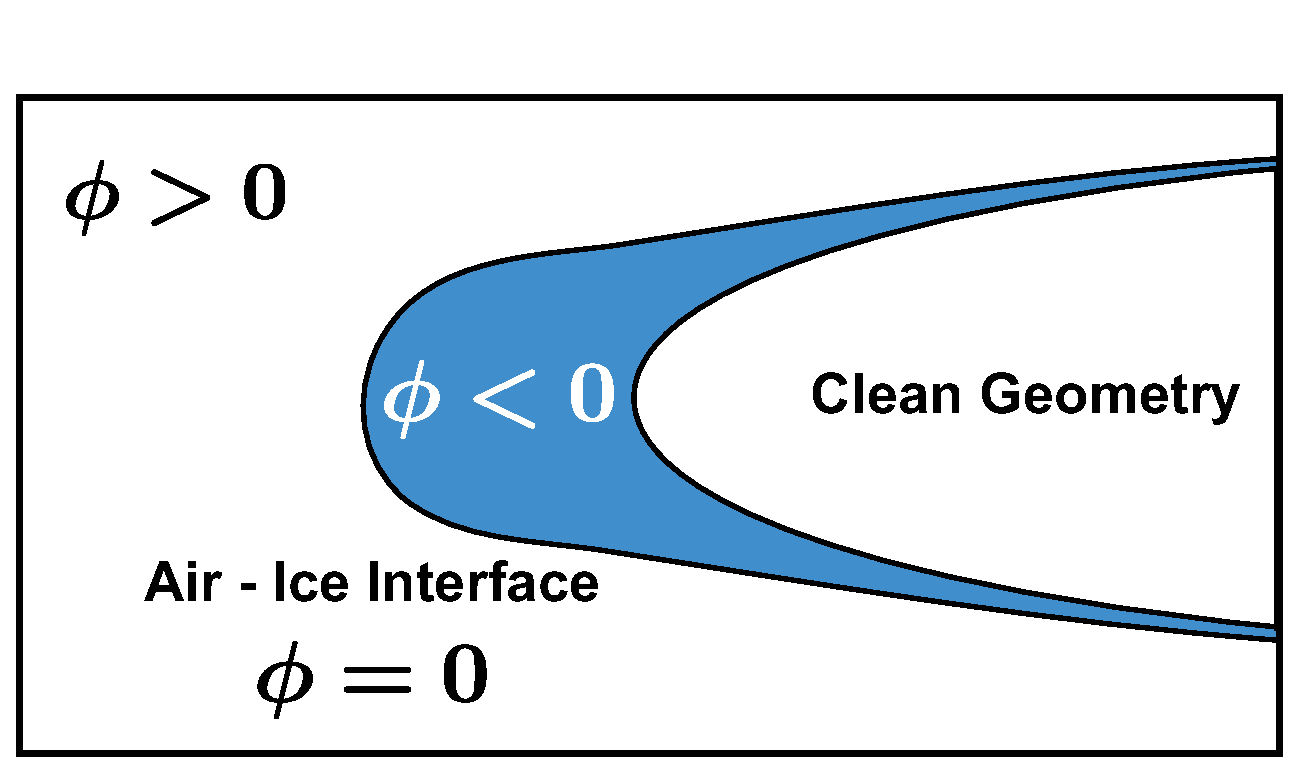
\includegraphics[width=\linewidth,height=3.68cm,keepaspectratio]{FIGURES/LEVELSET/ICE_AIR_INTERFACE}
  \end{column}
\end{columns}
\vspace{0.20cm}
\begin{center}
  {\color{champsBlue}\bfseries Evolve a field rather than moving surface nodes}
  \vspace{-0.13cm}
  \[
    \frac{\partial\phi}{\partial t}+\mathbf V\cdot\nabla\phi=0
  \]
\end{center}
\end{frame}

% ---------------------------------------------------------------
% 3 — NUMERICAL FORMULATION
% ---------------------------------------------------------------
\begin{frame}[t]{Level-Set Transport: Numerical Formulation}
\vspace{0.10cm}
\begin{center}
{\color{champsBlue}\bfseries Divergence form with a velocity-divergence correction}
\vspace{-0.13cm}
\[
\boxed{
\frac{\partial\phi}{\partial t}
+\nabla\cdot(\phi\mathbf V)
-\phi\,\nabla\cdot\mathbf V=0
}
\]
\end{center}
\vspace{-0.35cm}
\begin{columns}[T,onlytextwidth]
 \begin{column}{0.46\textwidth}
   {\color{champsBlue}\bfseries Ice-Growth Velocity}
   \vspace{-0.06cm}
   \[
     \mathbf V=\frac{h_{\mathrm{ice}}}{\Delta t_{\mathrm{layer}}}
     \mathbf n_{\phi_0},\qquad
     \mathbf n_{\phi_0}=\frac{\nabla\phi_0}{\lVert\nabla\phi_0\rVert}
   \]
   \vspace{0.08cm}
   \small
   Ice thickness is extended along the initial
   level-set normal direction, limiting redistancing needs
   for small layer displacements.
   \vspace{0.18cm}

   {\color{champsBlue}\bfseries Temporal Integration}
   \vspace{0.07cm}

   \small Semi-implicit \textbf{ROS22} (Rosenbrock--Wanner).
 \end{column}
 \hfill
 \begin{column}{0.50\textwidth}
   {\color{champsBlue}\bfseries Cell-Centered Finite Volumes}
   \vspace{-0.06cm}
   {\small
   \[
   \frac{\mathrm d\phi_i}{\mathrm dt}+R_i(\phi)=0
   \]
   \vspace{-0.17cm}
   \[
   R_i(\phi)=\frac{1}{|\Omega_i|}\sum_{f}
     (\phi_f-\phi_i)(\mathbf V_f\cdot\mathbf n_f)A_f
   \]
   }
   \vspace{0.04cm}
   \small
   \textbf{Spatial reconstruction:} second-order upwind;
   weighted least-squares gradients;
   Venkatakrishnan limiter.
 \end{column}
\end{columns}
\end{frame}

% ---------------------------------------------------------------
% 4 — INITIALIZATION AND SURFACE-VARIABLE EXTENSION
% ---------------------------------------------------------------
\begin{frame}[t]{Initialization and Extension of Surface Quantities}
\vspace{0.09cm}
\begin{columns}[T,onlytextwidth]
  \begin{column}{0.32\textwidth}
    \centering
    {\color{champsBlue}\bfseries Signed-Distance Initialization}
    \vspace{0.10cm}

    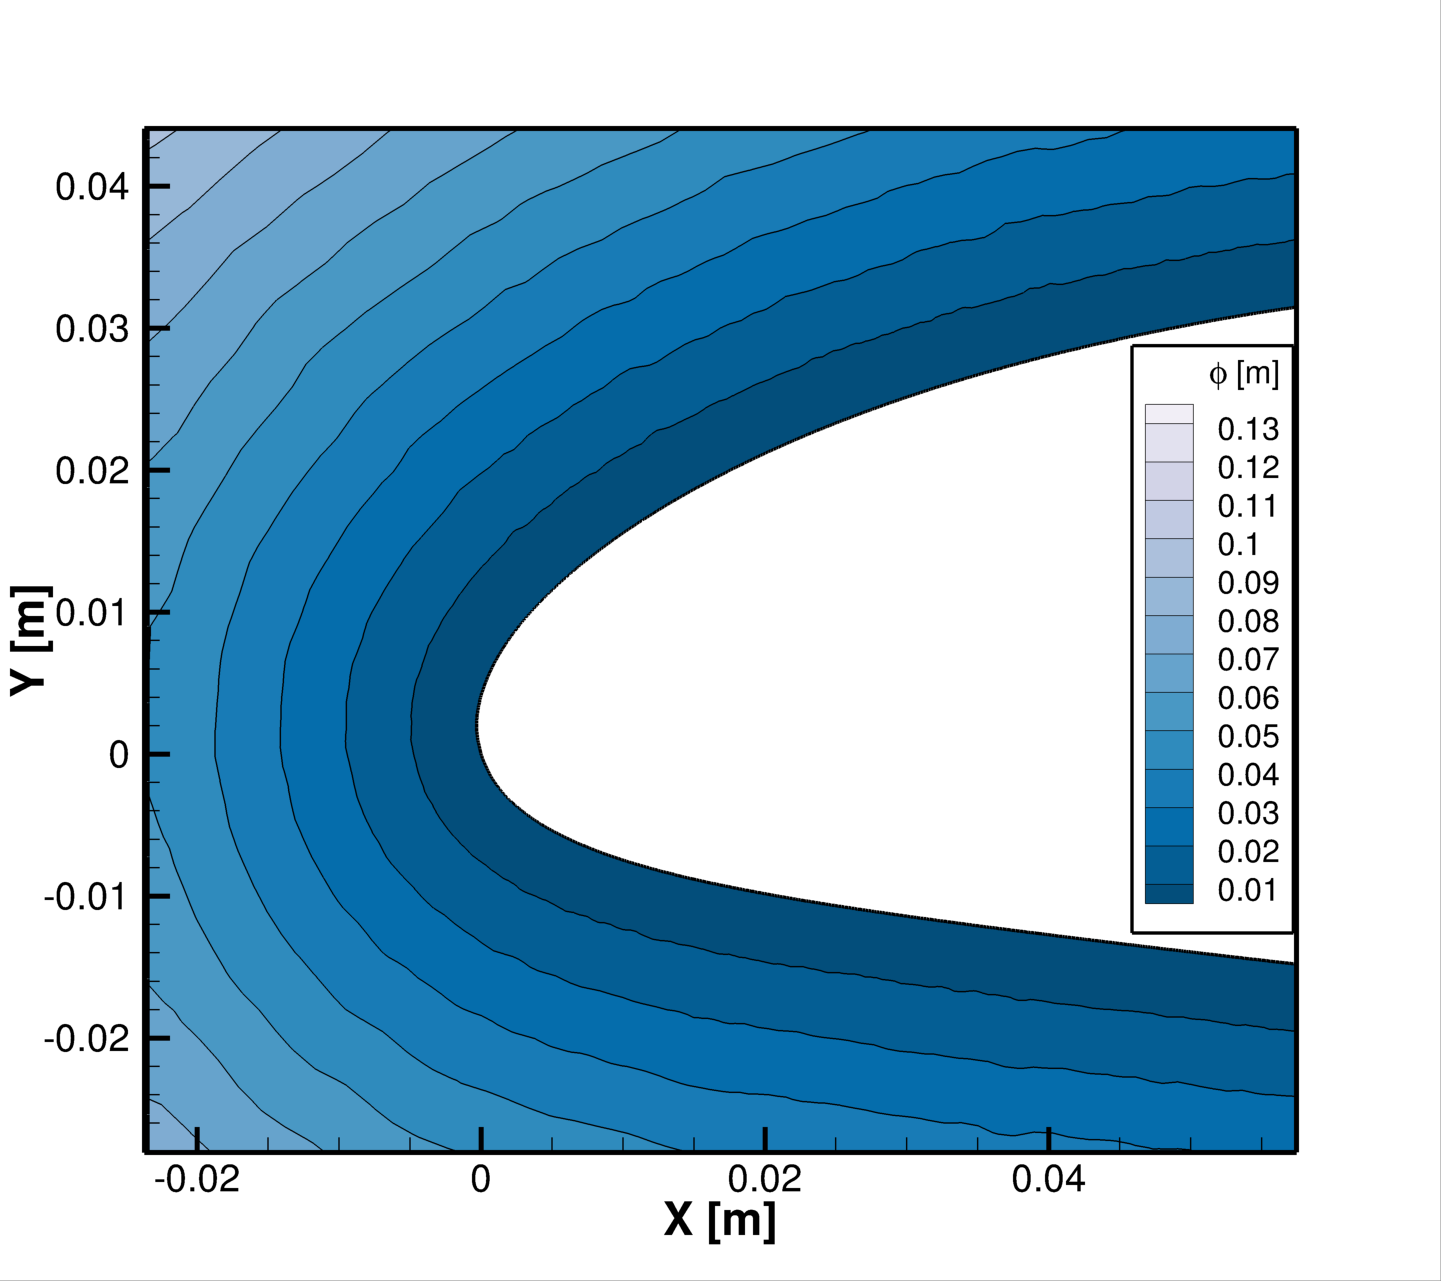
\includegraphics[width=\linewidth,height=2.28cm,keepaspectratio]{FIGURES/LEVELSET/EIKONAL.png}
    \vspace{-0.13cm}
    {\scriptsize
    \[
      \frac{\partial\phi}{\partial\tau}+
      \mathbf n_\phi\cdot\nabla\phi=1
    \]
    }
    \raggedright\scriptsize
    Eikonal pseudo-time transport with $\phi=0$ on the wall.
  \end{column}
  \hfill
  \begin{column}{0.32\textwidth}
    \centering
    {\color{champsBlue}\bfseries Ice-Thickness Extension}
    \vspace{0.10cm}

    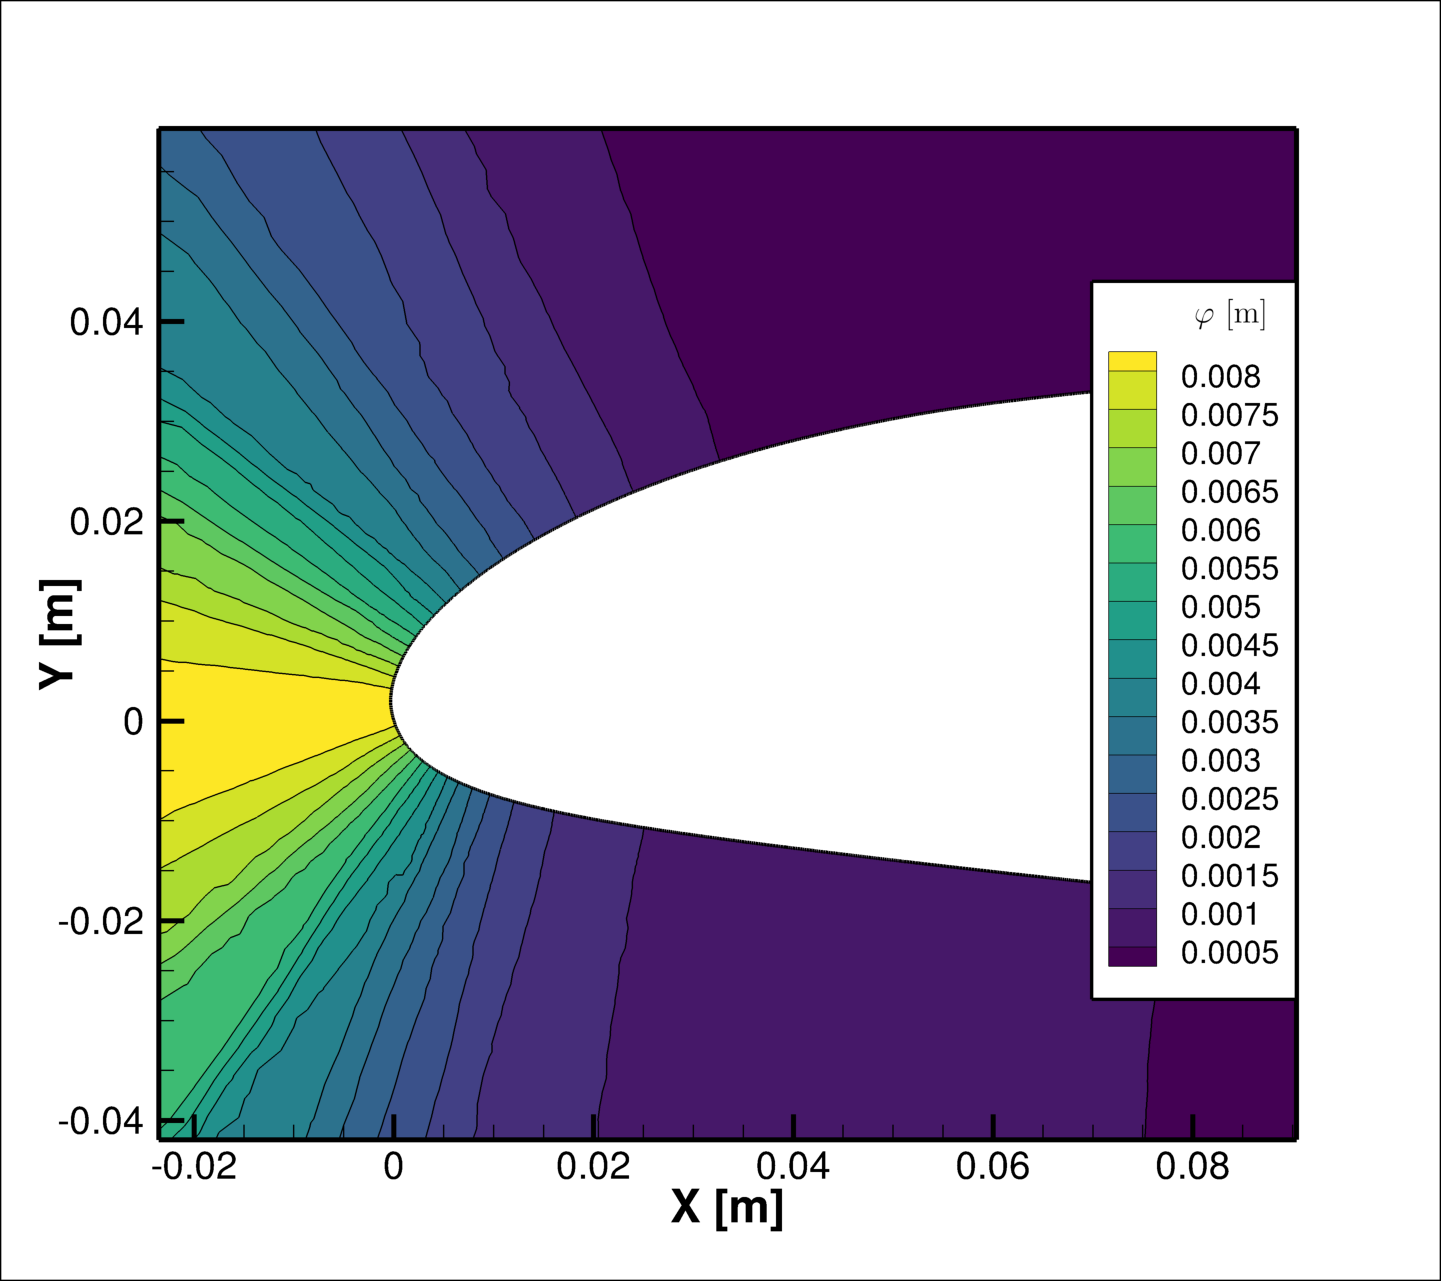
\includegraphics[width=\linewidth,height=2.28cm,keepaspectratio]{FIGURES/LEVELSET/PROPAGATION.png}
    \vspace{-0.13cm}
    {\scriptsize
    \[
      \frac{\partial\psi}{\partial\tau}+
      \mathbf n_\phi\cdot\nabla\psi=0
    \]
    }
    \raggedright\scriptsize
    Propagate surface ice thickness along signed-distance normals.
  \end{column}
  \hfill
  \begin{column}{0.32\textwidth}
    \centering
    {\color{champsBlue}\bfseries Geometric Alternative}
    \vspace{0.10cm}

    \FigOrPlaceholder{FIGURES/LEVELSET/AABB_TREE}{width=\linewidth,height=2.28cm,keepaspectratio}{2.0cm}
    \vspace{-0.13cm}
    {\scriptsize
    \[
      \phi(\mathbf x)=\pm\min_{T\in\Gamma}
      d(\mathbf x,T)
    \]
    }
    \raggedright\scriptsize
    Nearest-surface projection, accelerated by an AABB tree.
  \end{column}
\end{columns}
\vfill
\begin{center}
\colorbox{champsBlue!8}{\parbox{0.93\textwidth}{\centering\small
\vspace{0.10cm}
\textbf{Present framework:} Eikonal initialization and transport-based extension.
\quad\textbf{Alternative:} geometric closest-point projection with efficient spatial search.
\vspace{0.10cm}}}
\end{center}
\end{frame}

% ---------------------------------------------------------------
% 5 — MULTILAYER WORKFLOW
% ---------------------------------------------------------------
\begin{frame}[t]{CHAMPS -- Multilayer Ice-Accretion Approach}
\vspace{0.09cm}
\begin{columns}[T,onlytextwidth]
 \begin{column}{0.31\textwidth}
  \centering
  {\color{champsBlue}\bfseries 1. Icing Solution}
  \vspace{0.10cm}

  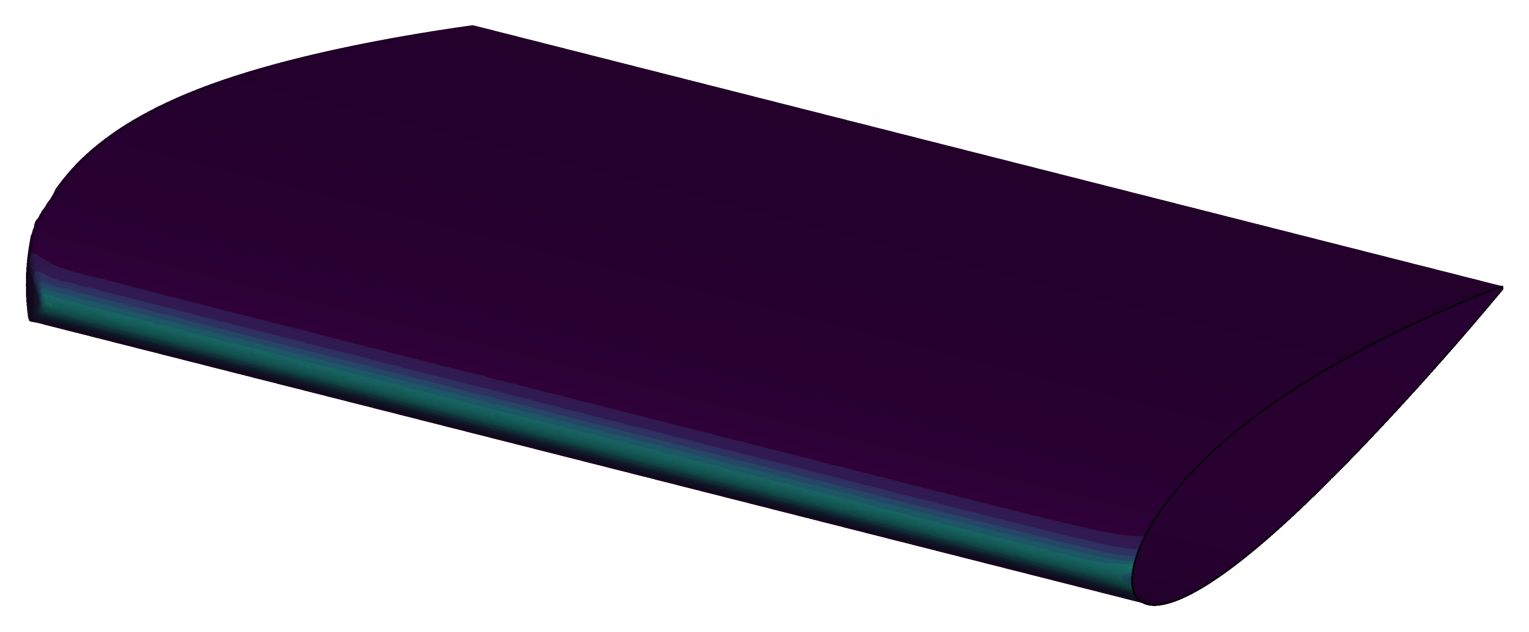
\includegraphics[width=\linewidth,height=2.40cm,keepaspectratio]{FIGURES/LEVELSET/THERMO_SOLUTION_CROP.png}
  \vspace{0.09cm}

  \raggedright\scriptsize
  \textbf{Flow $+$ droplets $+$ thermodynamics}
  \vspace{0.07cm}

  Obtain local ice mass accretion and thickness on the wing surface.
 \end{column}
 \hfill
 \begin{column}{0.31\textwidth}
  \centering
  {\color{champsBlue}\bfseries 2. Level-Set Evolution}
  \vspace{0.10cm}

  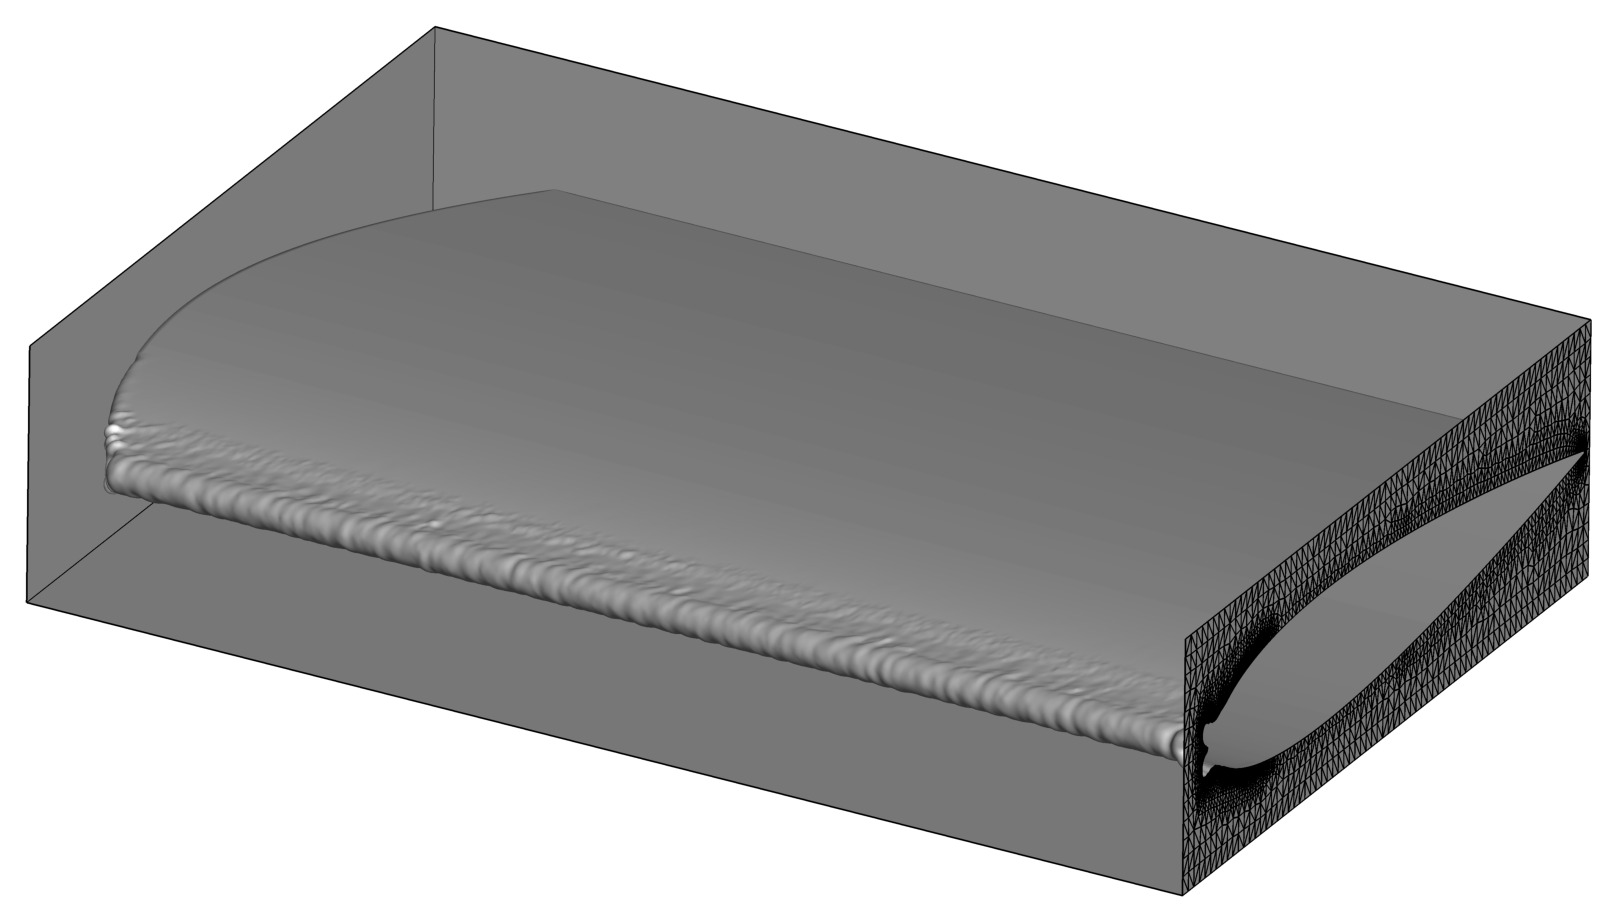
\includegraphics[width=\linewidth,height=2.40cm,keepaspectratio]{FIGURES/LEVELSET/LEVEL_SET_MESH_CROP.png}
  \vspace{0.09cm}

  \raggedright\scriptsize
  \textbf{Adapted auxiliary volume mesh}
  \vspace{0.07cm}

  $\sim$5--15 million cells; level-set transport $\sim$5 min per layer.
 \end{column}
 \hfill
 \begin{column}{0.31\textwidth}
  \centering
  {\color{champsBlue}\bfseries 3. Surface Reconstruction}
  \vspace{0.10cm}

  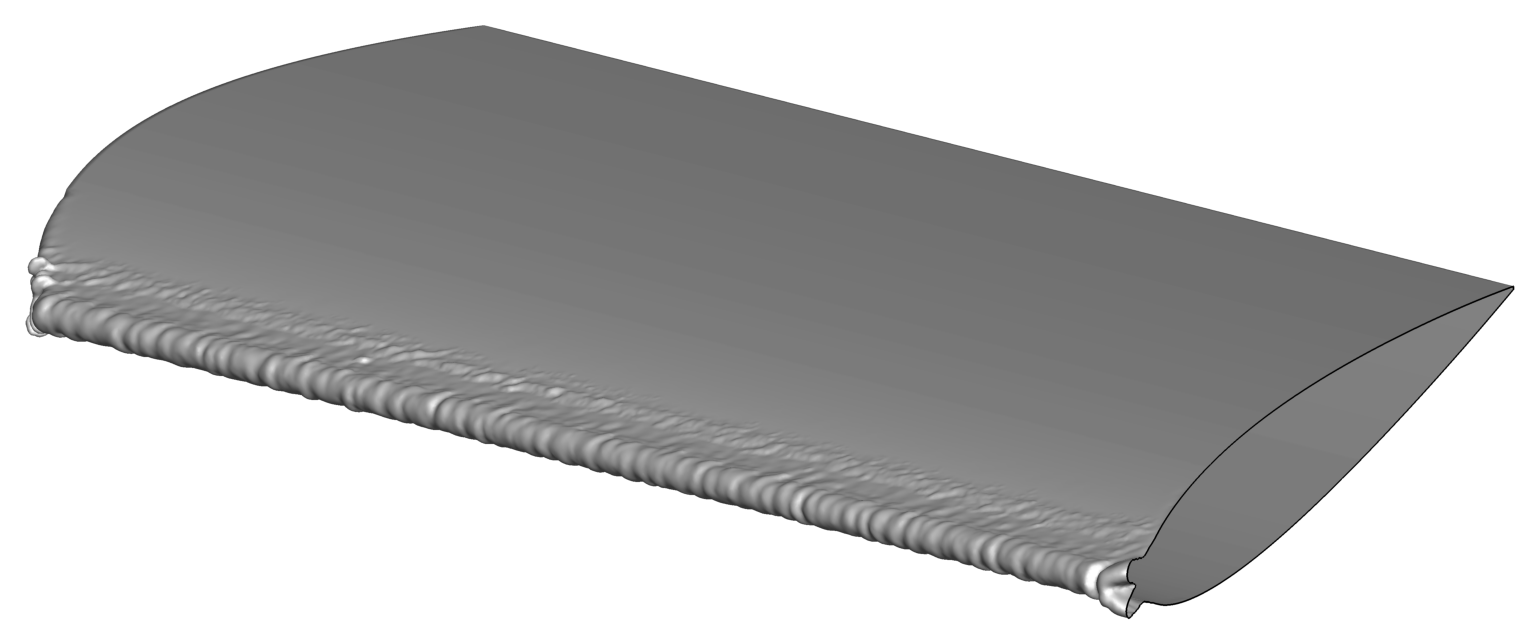
\includegraphics[width=\linewidth,height=2.40cm,keepaspectratio]{FIGURES/LEVELSET/LEVEL_SET_SURFACE_EXTRACTION_CROP.png}
  \vspace{0.09cm}

  \raggedright\scriptsize
  \textbf{MMG zero-isosurface extraction}
  \vspace{0.07cm}

  Surface smoothing and reconstruction; $\sim$20 min (serial bottleneck).
 \end{column}
\end{columns}
\vspace{0.32cm}
\begin{center}
\colorbox{champsBlue!8}{\parbox{0.92\textwidth}{\centering
\vspace{0.12cm}
{\color{champsBlue}\bfseries 4. Body-Fitted Volume Remeshing}
\vspace{0.07cm}

\small Automated Pointwise mesh update $\longrightarrow$
 recompute flow and impingement for the \textbf{next ice layer}.
\vspace{0.11cm}}}
\end{center}
\vfill
{\centering\tiny\color{gray}
Typical reported times vary with mesh size and workstation; 3D level set and extraction run locally.\par}
\end{frame}

% ---------------------------------------------------------------
% 6 — THREE-HORN BENCHMARK
% ---------------------------------------------------------------
\begin{frame}[t]{Three-Horn Benchmark: Geometry Robustness}
\vspace{0.13cm}
\begin{columns}[c,onlytextwidth]
 \begin{column}{0.64\textwidth}
  \centering
  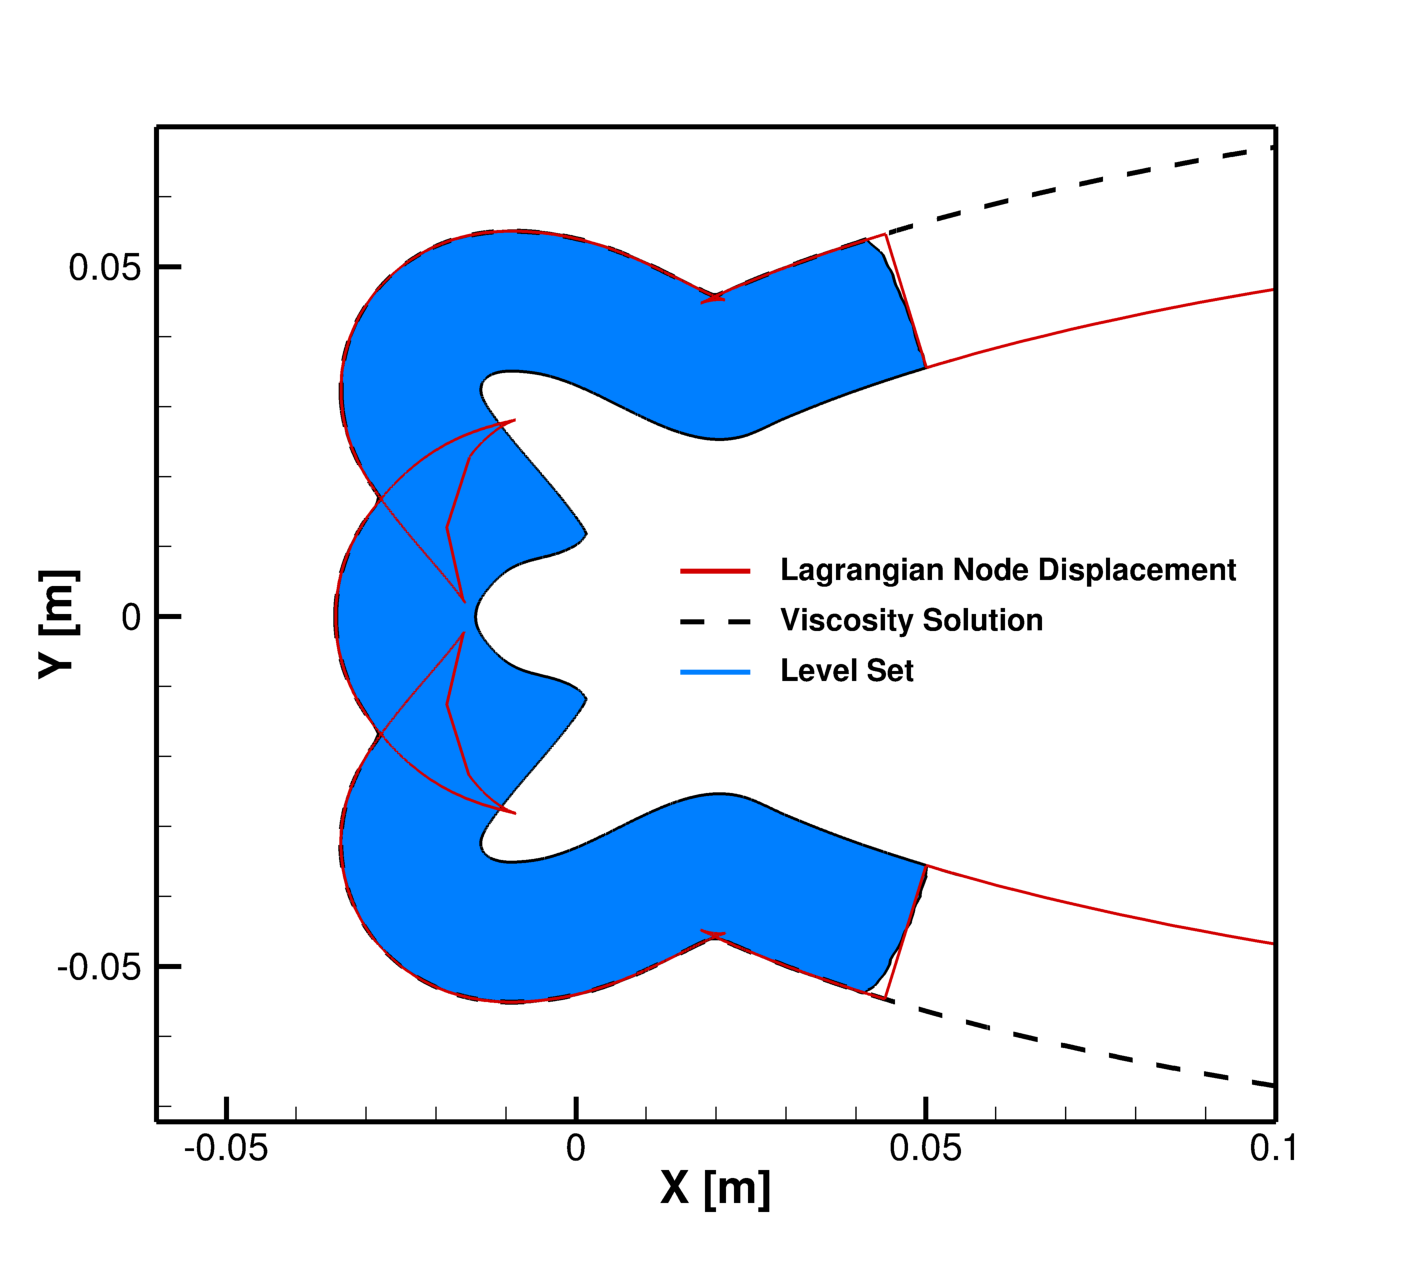
\includegraphics[width=\linewidth,height=5.00cm,keepaspectratio]{FIGURES/LEVELSET/THREE_HORNS.png}
 \end{column}
 \hfill
 \begin{column}{0.33\textwidth}
  {\color{champsBlue}\bfseries Manufactured Offset}
  \vspace{0.05cm}
  {\small\[
     h_{\mathrm{ice}}=0.02\,\mathrm m
     \qquad (x<0.05\,\mathrm m)
  \]}
  \vspace{0.13cm}
  {\color{red!75!black}\bfseries Direct Node Displacement}
  \vspace{0.06cm}
  \small Surface self-intersections and local ice-volume loss.
  \vspace{0.24cm}

  {\color{champsBlue}\bfseries Level-Set Evolution}
  \vspace{0.06cm}
  \small Reconstructs a valid front close to the exact geometric offset (viscosity solution).
 \end{column}
\end{columns}
\vfill
\begin{center}
\colorbox{champsBlue!8}{\parbox{0.92\textwidth}{\centering\small
\vspace{0.10cm}Implicit evolution handles concave, merging ice features without explicit surface entanglement.
\vspace{0.10cm}}}
\end{center}
\end{frame}

% ---------------------------------------------------------------
% 7 — IPW1 CASE 362: THREE-DIMENSIONAL MORPHOLOGY
% ---------------------------------------------------------------
\begin{frame}[t]{IPW1 Case 362: Three-Dimensional Scallop Formation}
\vspace{0.05cm}
{\centering\scriptsize
30$^\circ$ swept NACA 0012 \; $\vert$ \;
$T_\infty=266$ K \; $\vert$ \; 20 min icing \; $\vert$ \;
10 accretion layers
\par}
\vspace{0.10cm}
\begin{columns}[c,onlytextwidth]
  \begin{column}{0.42\textwidth}
    \centering
    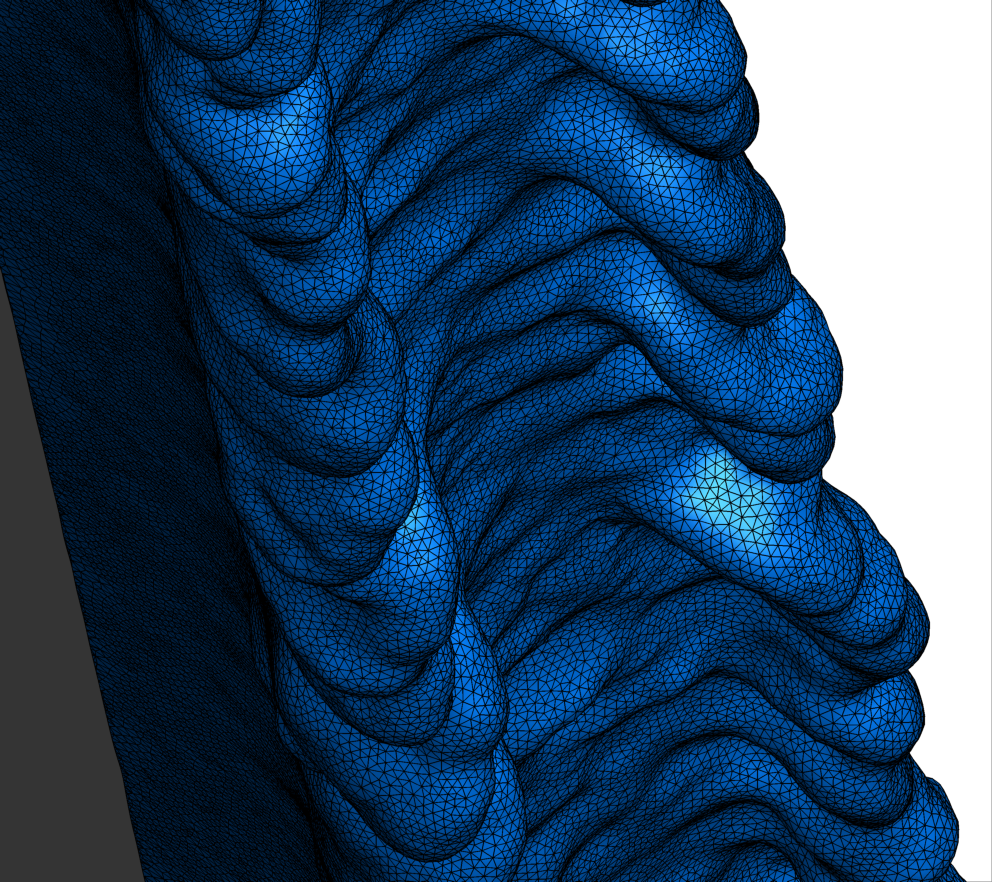
\includegraphics[width=\linewidth,height=4.40cm,keepaspectratio]{FIGURES/LEVELSET/CLIPPED_ICE_SHAPE_CASE_362_3.png}\par
    \vspace{0.04cm}
    {\scriptsize\color{gray}Scallops and adapted surface mesh.}
  \end{column}
  \hfill
  \begin{column}{0.55\textwidth}
    \centering
    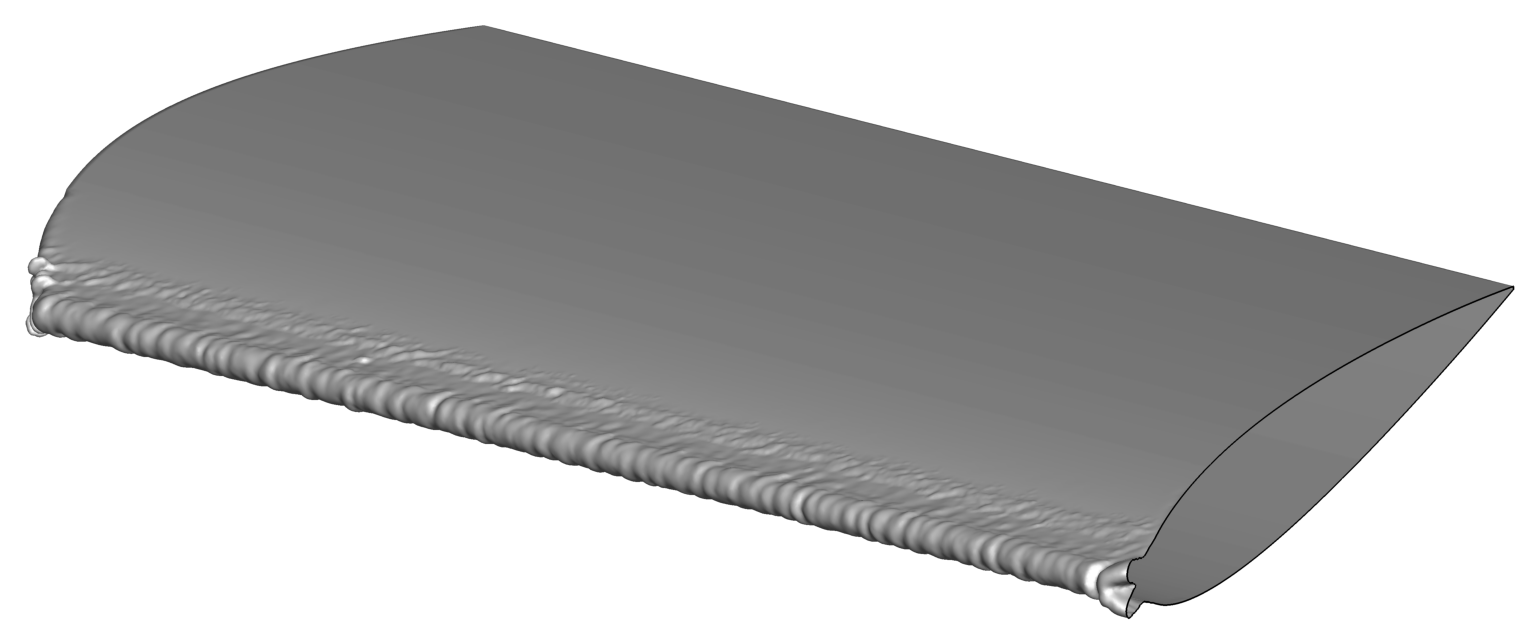
\includegraphics[width=\linewidth,height=4.30cm,keepaspectratio]{FIGURES/LEVELSET/LEVEL_SET_SURFACE_EXTRACTION_CROP.png}\par
    \vspace{0.04cm}
    {\scriptsize\color{gray}Reconstructed three-dimensional ice geometry.}
  \end{column}
\end{columns}
\vfill
\begin{center}
\colorbox{champsBlue!8}{\parbox{0.93\textwidth}{\centering\small
\vspace{0.11cm}Multilayer level-set evolution captures complex
spanwise ice features while maintaining a conformal extracted surface.
\vspace{0.11cm}}}
\end{center}
\end{frame}

% ---------------------------------------------------------------
% 8 — IPW1 CASE 362: CROSS SECTION / EXPERIMENT
% ---------------------------------------------------------------
\begin{frame}[t]{IPW1 Case 362: Ice-Shape Comparison}
\vspace{0.07cm}
{\centering\scriptsize
30$^\circ$ swept NACA 0012 \; $\vert$ \;
LWC = 0.5 g/m$^3$ \; $\vert$ \;
MVD = 34.7 $\mu$m \; $\vert$ \;
$k_s/c=0.001$
\par}
\vspace{0.14cm}
\begin{columns}[c,onlytextwidth]
  \begin{column}{0.65\textwidth}
    \centering
    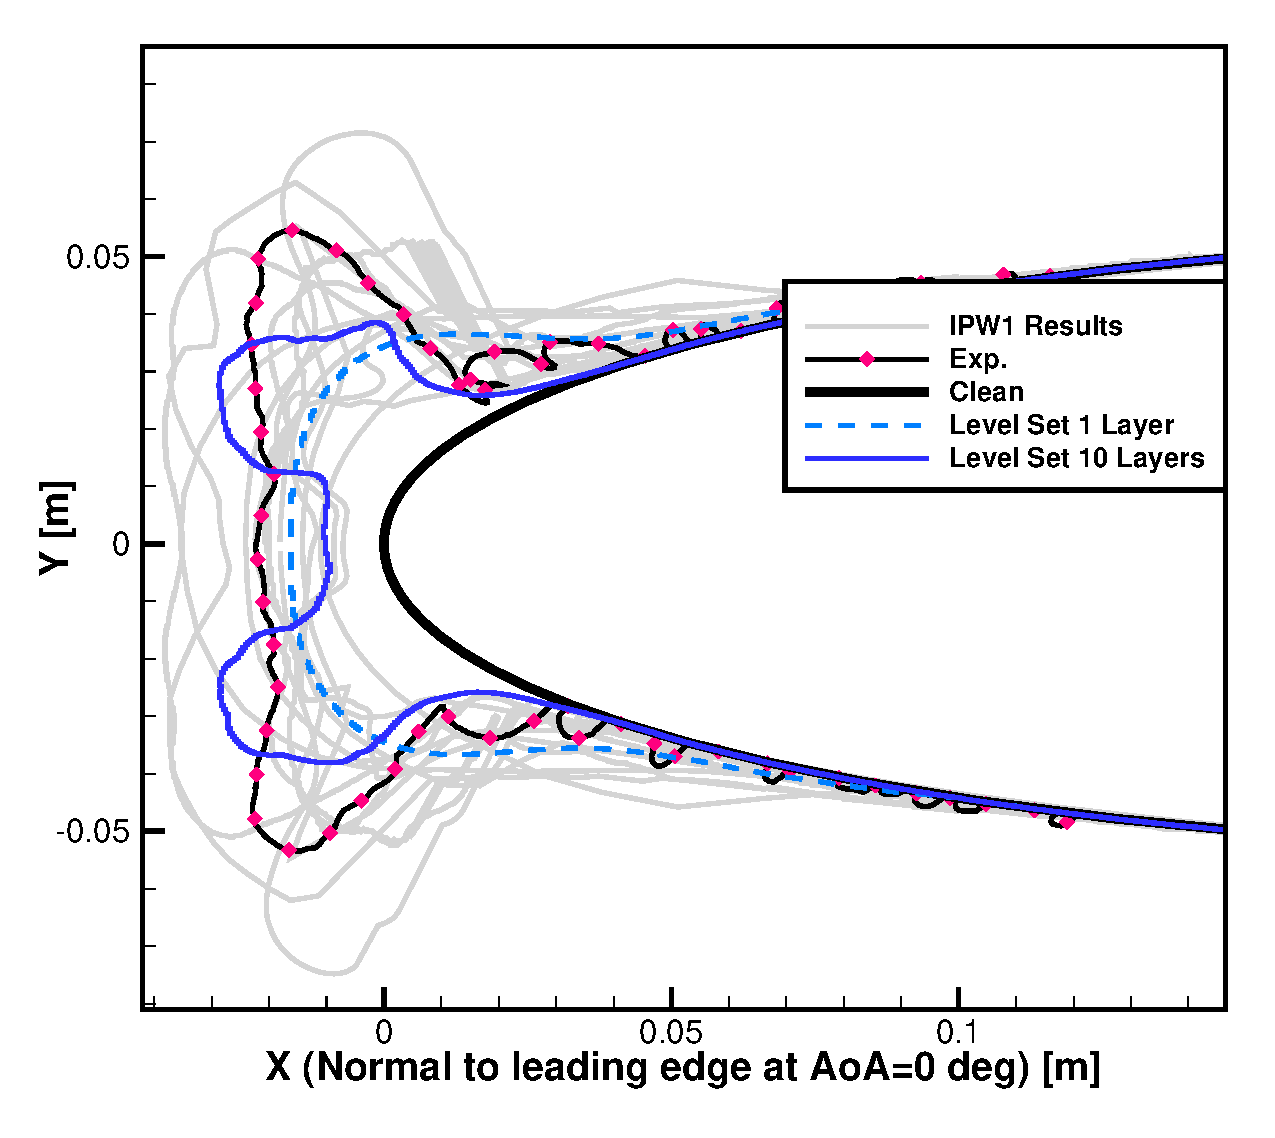
\includegraphics[width=\linewidth,height=4.82cm,keepaspectratio]{FIGURES/LEVELSET/CASE_IPW1_362_ICE_SHAPE}
  \end{column}
  \hfill
  \begin{column}{0.32\textwidth}
    {\color{champsBlue}\bfseries Single Step vs. 10 Layers}
    \vspace{0.10cm}

    \small Multilayer predictions reproduce horn and scallop development
    not captured in one step.
    \vspace{0.30cm}

    {\color{champsBlue}\bfseries Experimental Comparison}
    \vspace{0.10cm}

    \small Reasonably good overall agreement of the
    maximum combined cross section (MCCS).
    \vspace{0.25cm}

    {\color{red!70!black}\bfseries Remaining Discrepancies}
    \vspace{0.10cm}

    \small Horn orientation and impingement limits.
  \end{column}
\end{columns}
\vfill
\begin{center}
\colorbox{champsBlue!8}{\parbox{0.92\textwidth}{\centering\small
\vspace{0.10cm}2D MCCS comparisons do not fully reveal the local spanwise variation
of genuinely three-dimensional ice structures.\vspace{0.10cm}}}
\end{center}
\end{frame}


\section[IBM]{Immersed Boundary Method}

% Section transition: 05_HYBRID_IMMERSED_BOUNDARY_METHOD
\definecolor{meshGrey}{RGB}{211,211,211}
{\renewcommand{\iceImgX}{1.2}\renewcommand{\iceImgY}{0.50}\renewcommand{\iceImgBg}{meshGrey}%
\IceSectionDivider[height=1.15\H]{}{Immersed\\ Boundary Method}{FIGURES/SECTION_TRANSITION/iceMeshLE_IBM_LAST_LAYER_ADAPTED.png}}


% ---------------------------------------------------------
% Immersed-boundary methods: main approaches
% ---------------------------------------------------------
\begin{frame}{Immersed-Boundary Methods: Main Approaches}

\vspace{0.08cm}

\noindent\resizebox{\textwidth}{!}{Immersed-boundary methods represent solid geometries
without requiring a body-fitted computational mesh.}

\vspace{0.28cm}

\begin{columns}[T,onlytextwidth]

% CUT-CELL
\begin{column}{0.31\textwidth}
\centering
{\color{champsBlue}\bfseries Cut-Cell Method}

\vspace{0.15cm}

\parbox[c][3.0cm][c]{\linewidth}{\centering
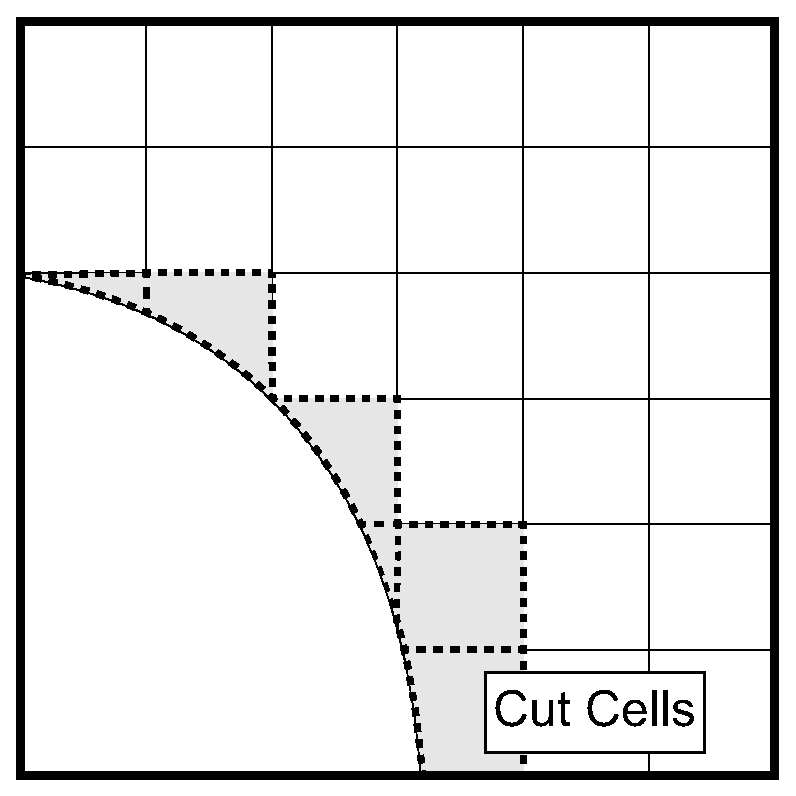
\includegraphics[width=0.96\linewidth,height=2.95cm,keepaspectratio]{FIGURES/IBM/CUT_CELL.eps}
}

\vspace{0.15cm}

\parbox{\linewidth}{\small\raggedright
Modifies intersected control volumes
to conform to the immersed boundary.
}
\end{column}

% PENALIZATION
\begin{column}{0.31\textwidth}
\centering
{\color{champsBlue}\bfseries Penalization Method}

\vspace{0.15cm}

\parbox[c][3.0cm][c]{\linewidth}{\centering
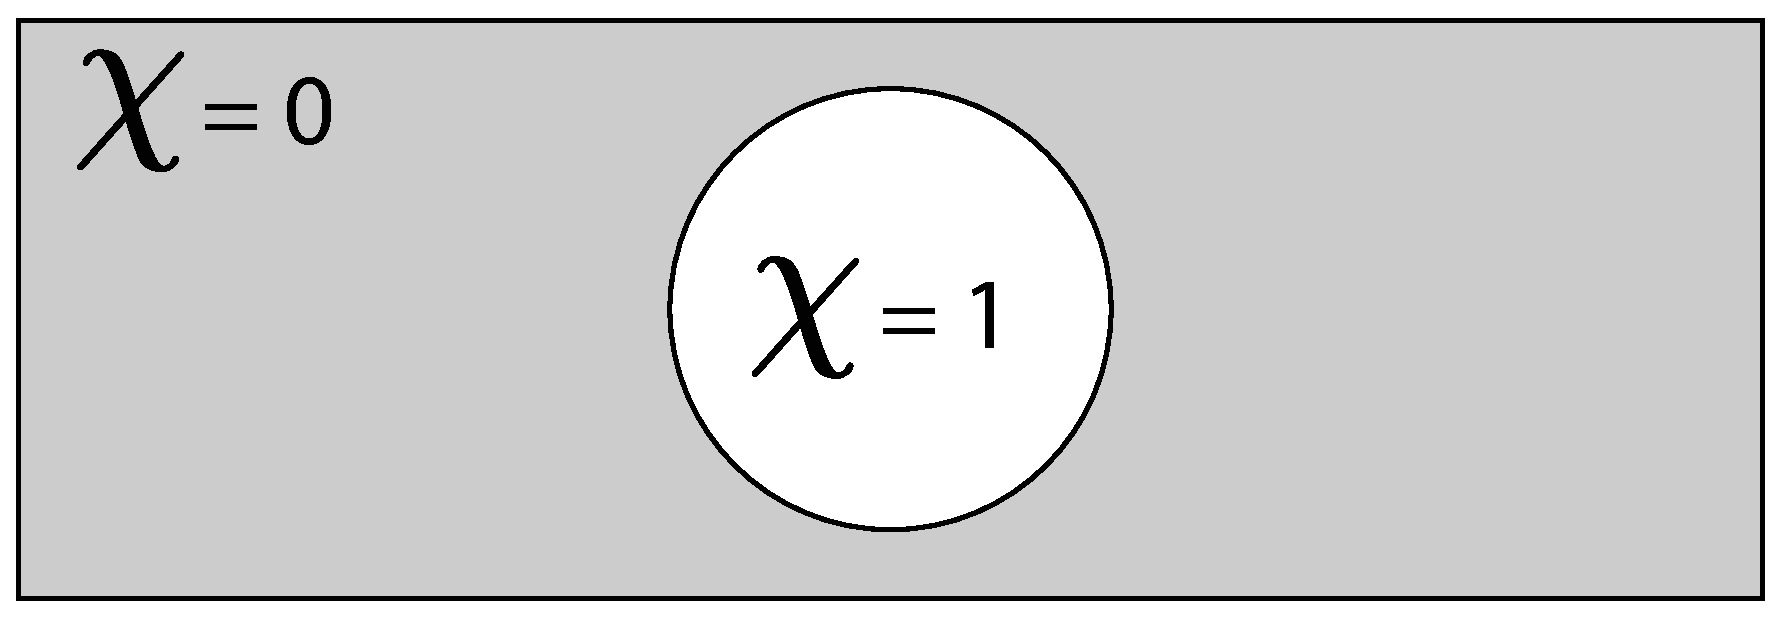
\includegraphics[width=\linewidth,height=2.95cm,keepaspectratio]{FIGURES/IBM/SIMPLIFIED_MASK.eps}
}

\vspace{0.15cm}

\parbox{\linewidth}{\small\raggedright
Introduces source terms to enforce
boundary behavior within the solid region.
}
\end{column}

% GHOST-CELL
\begin{column}{0.31\textwidth}
\centering
{\color{champsBlue}\bfseries Ghost-Cell Method}

\vspace{0.15cm}

\parbox[c][3.0cm][c]{\linewidth}{\centering
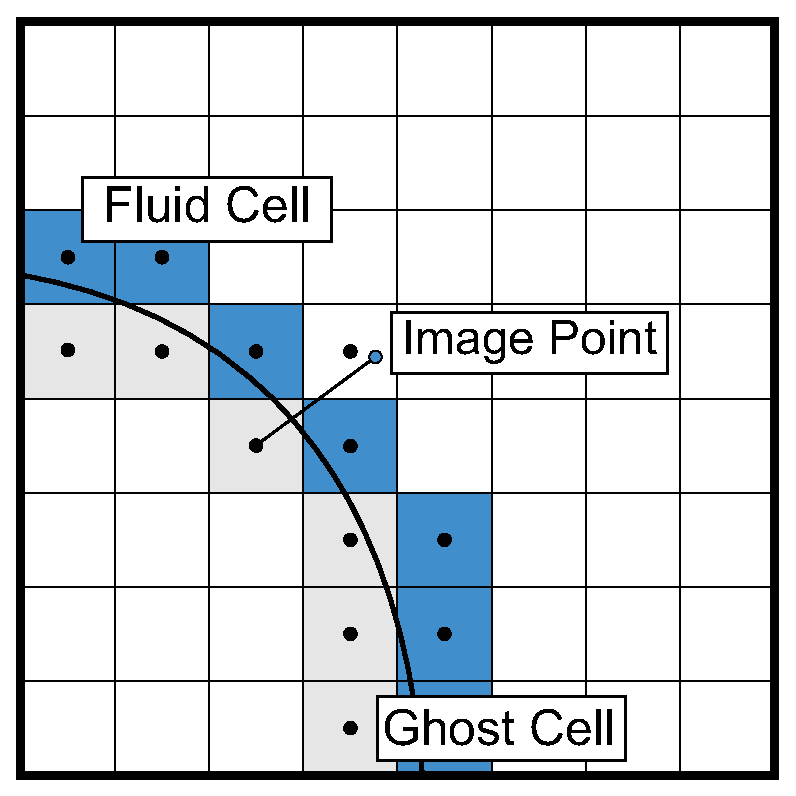
\includegraphics[width=0.96\linewidth,height=2.95cm,keepaspectratio]{FIGURES/IBM/SIMPLIFIED_GC.eps}
}

\vspace{0.15cm}

\parbox{\linewidth}{\small\raggedright
Reconstructs ghost-cell states
to impose immersed-wall boundary conditions.
}
\end{column}

\end{columns}

\vfill

\begin{center}

\begin{tikzpicture}
\node[fill=champsBlue!5, draw=champsBlue!18, rounded corners=4pt,
      text width=0.92\textwidth, inner sep=3pt, align=center, font=\small] {%
\textbf{Existing CHAMPS capability:}
Ghost-cell immersed-boundary RANS solver.};
\end{tikzpicture}
\end{center}

\SlideRef{peskin1972flow,mittal2005immersed,fadlun2000combined,tseng2003ghost,angot1999penalization}
\end{frame}

% 2. EULERIAN IMMERSED DROPLET TREATMENT
\begin{frame}[t]{Eulerian Droplets: Penalization Strategy}
\vspace{-0.15cm}
\small Established penalization strategy integrated into the CHAMPS Eulerian droplet solver.
\par\vspace{0.1cm}
\begin{columns}[T,onlytextwidth]
  \begin{column}{0.32\textwidth}
  \centering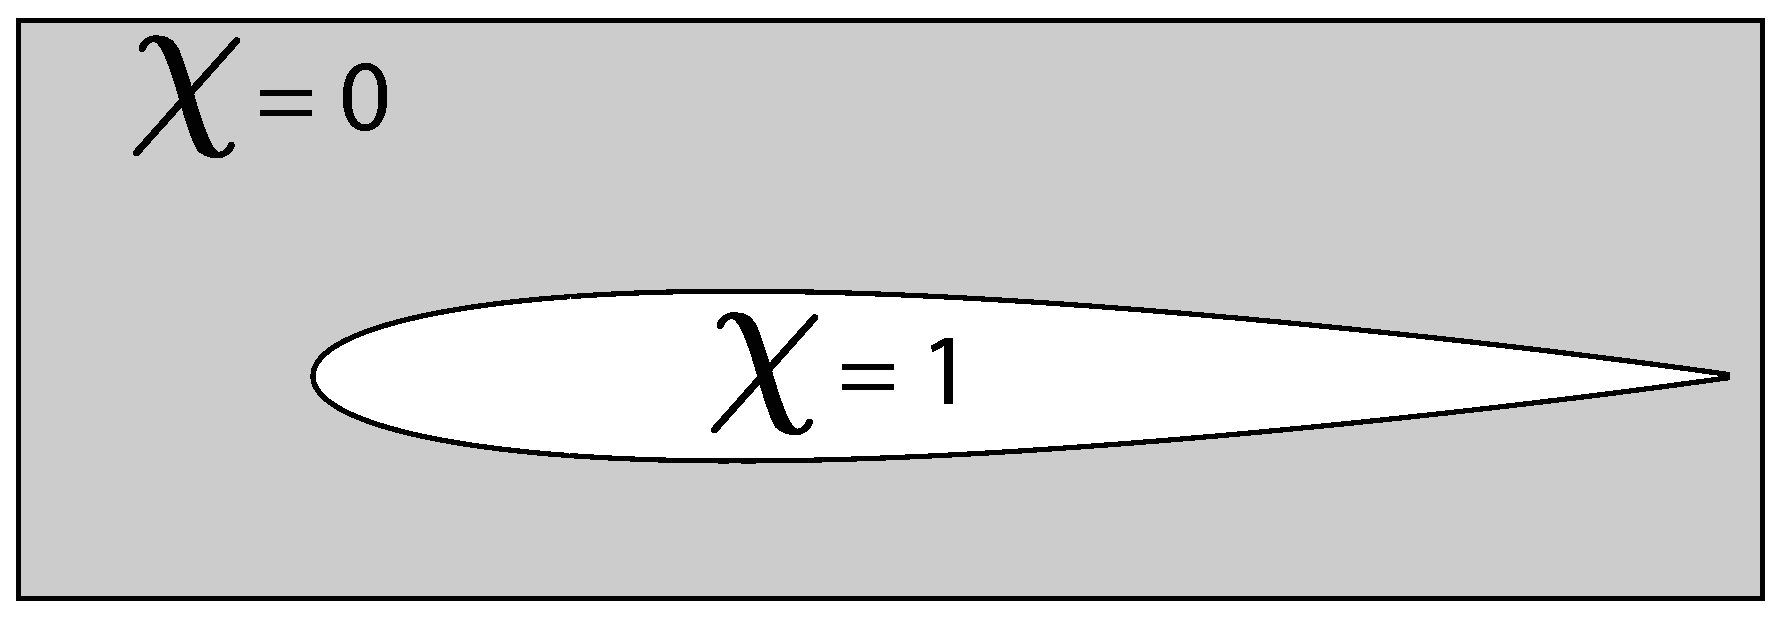
\includegraphics[width=\linewidth,height=1.0cm,keepaspectratio]{FIGURES/IBM/mask}\par
  \vspace{0.02cm}
  {\small\color{champsBlue}\bfseries Solid mask $\chi$}\par
  \end{column}
  \begin{column}{0.32\textwidth}
  \centering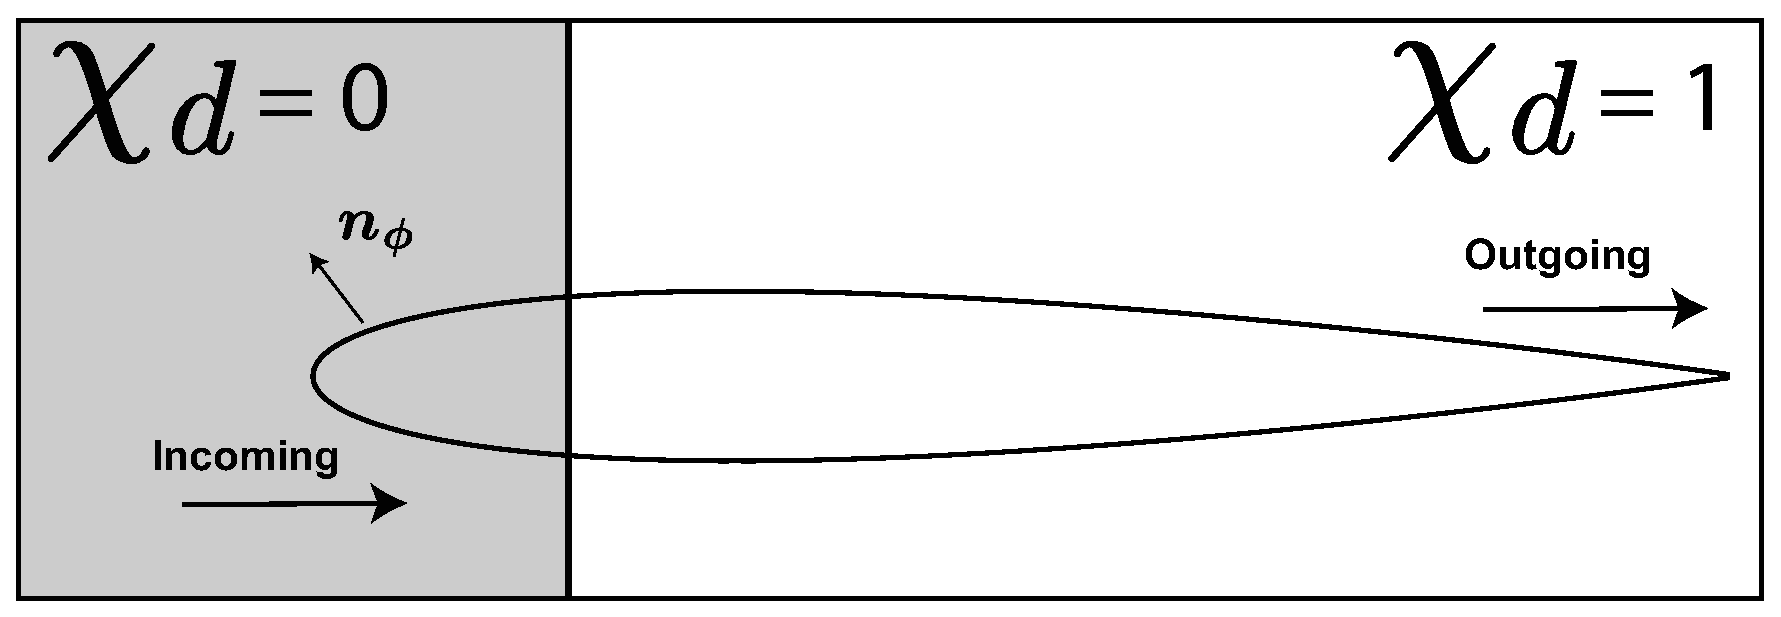
\includegraphics[width=\linewidth,height=1.0cm,keepaspectratio]{FIGURES/IBM/maskChiD}\par
  \vspace{0.02cm}
  {\small\color{champsBlue}\bfseries Direction mask $\chi_d$}\par
  \end{column}
  \begin{column}{0.32\textwidth}
  \centering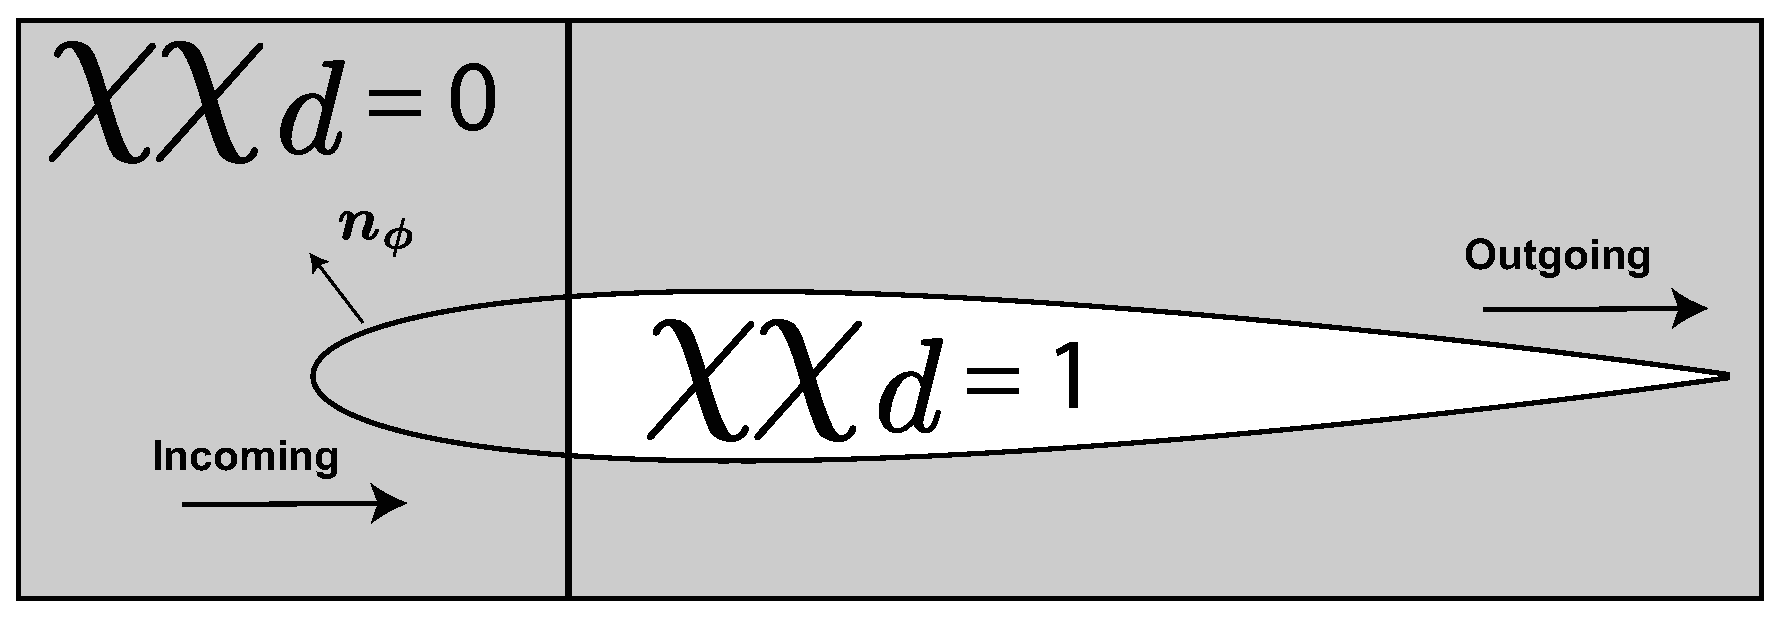
\includegraphics[width=\linewidth,height=1.0cm,keepaspectratio]{FIGURES/IBM/maskChiChiD}\par
  \vspace{0.02cm}
  {\small\color{champsBlue}\bfseries Active mask $\chi\chi_d$}\par
  \end{column}
\end{columns}
\par\vspace*{0.3cm}\mbox{}\par\vspace*{-0.3cm}
\begin{columns}[T,onlytextwidth]
\begin{column}{0.63\textwidth}
{\color{champsBlue}\bfseries Penalized Eulerian Droplet Equations}\par
\vspace{-0.12cm}
{\scriptsize
\begin{align*}
\frac{\partial \alpha}{\partial t}
+\nabla\cdot(\alpha\mathbf{u}_d)
&=
\textcolor{red!80!black}{-}\textcolor{red!80!black}{\underbrace{\frac{\chi\chi_d}{\eta}\alpha}_{\text{Penalization}}}
\\[0.04cm]
\frac{\partial(\alpha\mathbf{u}_d)}{\partial t}
+\nabla\cdot(\alpha\mathbf{u}_d\otimes\mathbf{u}_d)
&=
\textcolor{red!80!black}{(1-\chi)}\left[
\frac{C_DRe_D}{24St}\alpha(\mathbf{u}_a-\mathbf{u}_d)
+\alpha\left(1-\frac{\rho_a}{\rho_d}\right)
\frac{\mathbf{g}}{Fr^2}
\right]
\\
&\quad\textcolor{red!80!black}{-}
\textcolor{red!80!black}{\underbrace{\frac{\chi\chi_d}{\eta}\alpha\mathbf{u}_d}_{\text{Penalization}}}
\end{align*}}
\end{column}
\hfill
\begin{column}{0.34\textwidth}
{\color{champsBlue}\bfseries Direction Mask}\par
\vspace{0.04cm}
{\centering\scriptsize$\chi_d=\begin{cases}1, & \mathbf{u}_d\cdot\mathbf{n}_{\phi}\leq 0,\\ 0, & \mathbf{u}_d\cdot\mathbf{n}_{\phi}>0.\end{cases}$\par}
\vspace{0.1cm}
{\color{champsBlue}\bfseries Main Benefits}\par
\vspace{0.02cm}
\begin{itemize}\footnotesize\setlength{\itemsep}{1pt}
  \item Limited solver modifications.
  \item Body-fitted-like impingement predictions.
  \item Second-order spatial convergence recovered in verification.
\end{itemize}
\end{column}
\end{columns}
\vfill
\begin{center}

\begin{tikzpicture}
\node[fill=champsBlue!5, draw=champsBlue!18, rounded corners=4pt,
      text width=\textwidth-0.2cm, inner sep=3pt, align=center, font=\small] {%
\textbf{Penalization acts only in the incoming-droplet region inside the immersed body.}};
\end{tikzpicture}
\end{center}
\SlideRef{angot1999penalization,lavoieDroplets}
\end{frame}

% 3. LAGRANGIAN IMMERSED-SURFACE IMPACT DETECTION
\begin{frame}{Lagrangian Droplets: Immersed-Surface Impacts}
\vspace{0.06cm}
\begin{columns}[c,onlytextwidth]
\begin{column}{0.42\textwidth}
{\color{champsBlue}\bfseries Preserve Face-to-Face Tracking}\par
\vspace{0.10cm}
\begin{itemize}\setlength{\itemsep}{4pt}
  \item Advance trajectories through the \textbf{background volume mesh}.
  \item Pre-tag cells cut by the immersed surface.
  \item On entry, test the trajectory ray against associated surface facets.
  \item \textbf{Axis-Aligned Bounding Box (AABB) tree geometry queries} accelerate closest-point and intersection operations.
\end{itemize}
\vspace{0.15cm}
{\small\color{champsBlue}\bfseries Everything else is kept from the body-fitted solver; only the impact-position detection changes.\par}
\end{column}
\hfill
\begin{column}{0.55\textwidth}
\centering
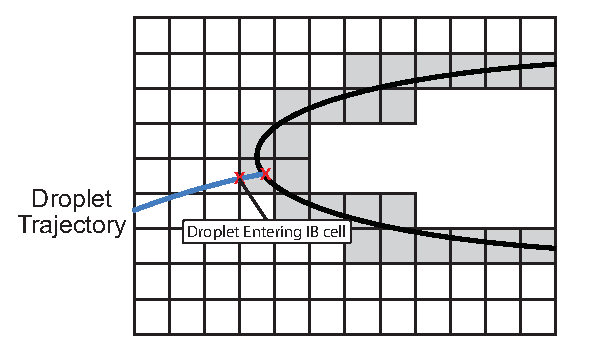
\includegraphics[width=\linewidth,height=5.0cm,keepaspectratio]{FIGURES/IBM/surfaceIntersection}\par
\vspace{0.06cm}
{\scriptsize\color{gray}Intersection of the droplet trajectory with the immersed surface.}
\end{column}
\end{columns}
\SlideRef{pabloThesis}
\end{frame}

% 4. IBM LEVEL-SET COUPLING
\begin{frame}[t]{IBM--Level-Set Icing Framework}
\vspace{0.04cm}
\small The \textbf{aerodynamic and droplet} fields use a nonconformal IBM background mesh;
\textbf{geometry evolution} retains an adapted, body-fitted auxiliary mesh.
\vspace{0.22cm}
\begin{center}
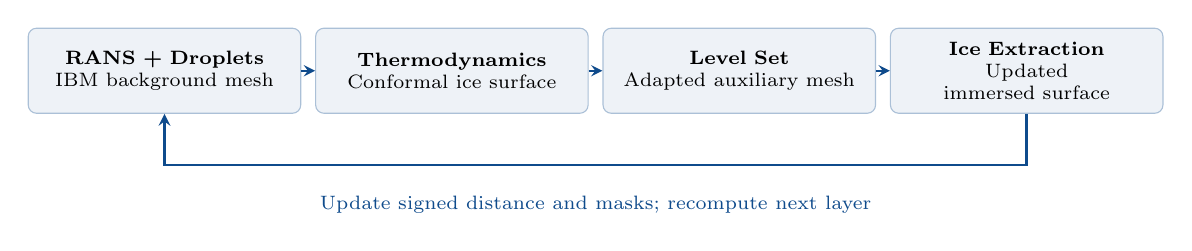
\begin{tikzpicture}[>=stealth,
    every node/.style={align=center,font=\scriptsize,execute at begin node={\hyphenpenalty=10000}},
    stage/.style={draw=champsBlue!35,fill=champsBlue!7,rounded corners=3pt,
       minimum height=1.08cm,text width=3.25cm,inner sep=3pt}]
  \node[stage] (flow) at (0,0) {\textbf{RANS + Droplets}\\IBM background mesh};
  \node[stage] (thermo) at (3.65,0) {\textbf{Thermodynamics}\\Conformal ice surface};
  \node[stage] (ls) at (7.30,0) {\textbf{Level Set}\\Adapted auxiliary mesh};
  \node[stage] (geom) at (10.95,0) {\textbf{Ice Extraction}\\Updated immersed surface};
  \draw[->,line width=0.8pt,champsBlue] (flow)--(thermo);
  \draw[->,line width=0.8pt,champsBlue] (thermo)--(ls);
  \draw[->,line width=0.8pt,champsBlue] (ls)--(geom);
  \draw[->,line width=0.9pt,champsBlue] (geom.south) -- ++(0,-0.65) -| (flow.south);
  \node[fill=white,text=champsBlue,font=\scriptsize] at (5.475,-1.70)
  {Update signed distance and masks; recompute next layer};
\end{tikzpicture}
\end{center}
\vspace{0.16cm}
\begin{columns}[T,onlytextwidth]
\begin{column}{0.48\textwidth}
{\color{champsBlue}\bfseries Why Keep the Level-Set Mesh Body-Fitted?}\par
\vspace{0.10cm}
\small The auxiliary level-set mesh is easier to adapt than a RANS
mesh, since no thin boundary-layer cells are required.
\end{column}
\hfill
\begin{column}{0.48\textwidth}
{\color{champsBlue}\bfseries Preserve the Clean Geometry}\par
\vspace{0.10cm}
\small Restrict evolution and reconstruction to the ice-growth region;
retain unaffected geometry rather than moving the full interface.
\end{column}
\end{columns}
\vfill
\begin{center}

\begin{tikzpicture}
\node[fill=champsBlue!5, draw=champsBlue!18, rounded corners=4pt,
      text width=0.92\textwidth, inner sep=3pt, align=center, font=\small] {%
\textbf{Avoid repeated body-fitted RANS remeshing, not all auxiliary meshing.}};
\end{tikzpicture}
\end{center}
\SlideRef{lavoieLevelSet,lavoie2021immersed,pabloThesis}
\end{frame}

% 5. SLD NACA 23012
\begin{frame}[t]{IBM Impingement Results: NACA 23012 (SLD)}
\vspace{-0.3cm}
\begin{center}
{\scriptsize\color{champsBlue}\bfseries NACA 23012 \quad
$\bm{M_\infty=0.232}$ \quad \textbf{AoA} $\bm{=2.5^\circ}$ \quad
LWC $=0.50$ g/m$^3$ \quad MVD $=111\,\mu$m}
\end{center}
\vspace{0.06cm}
\begin{columns}[T,onlytextwidth]
  \begin{column}{0.49\textwidth}
    \centering
    {\color{champsBlue}\bfseries Eulerian}\par\vspace{0.08cm}
    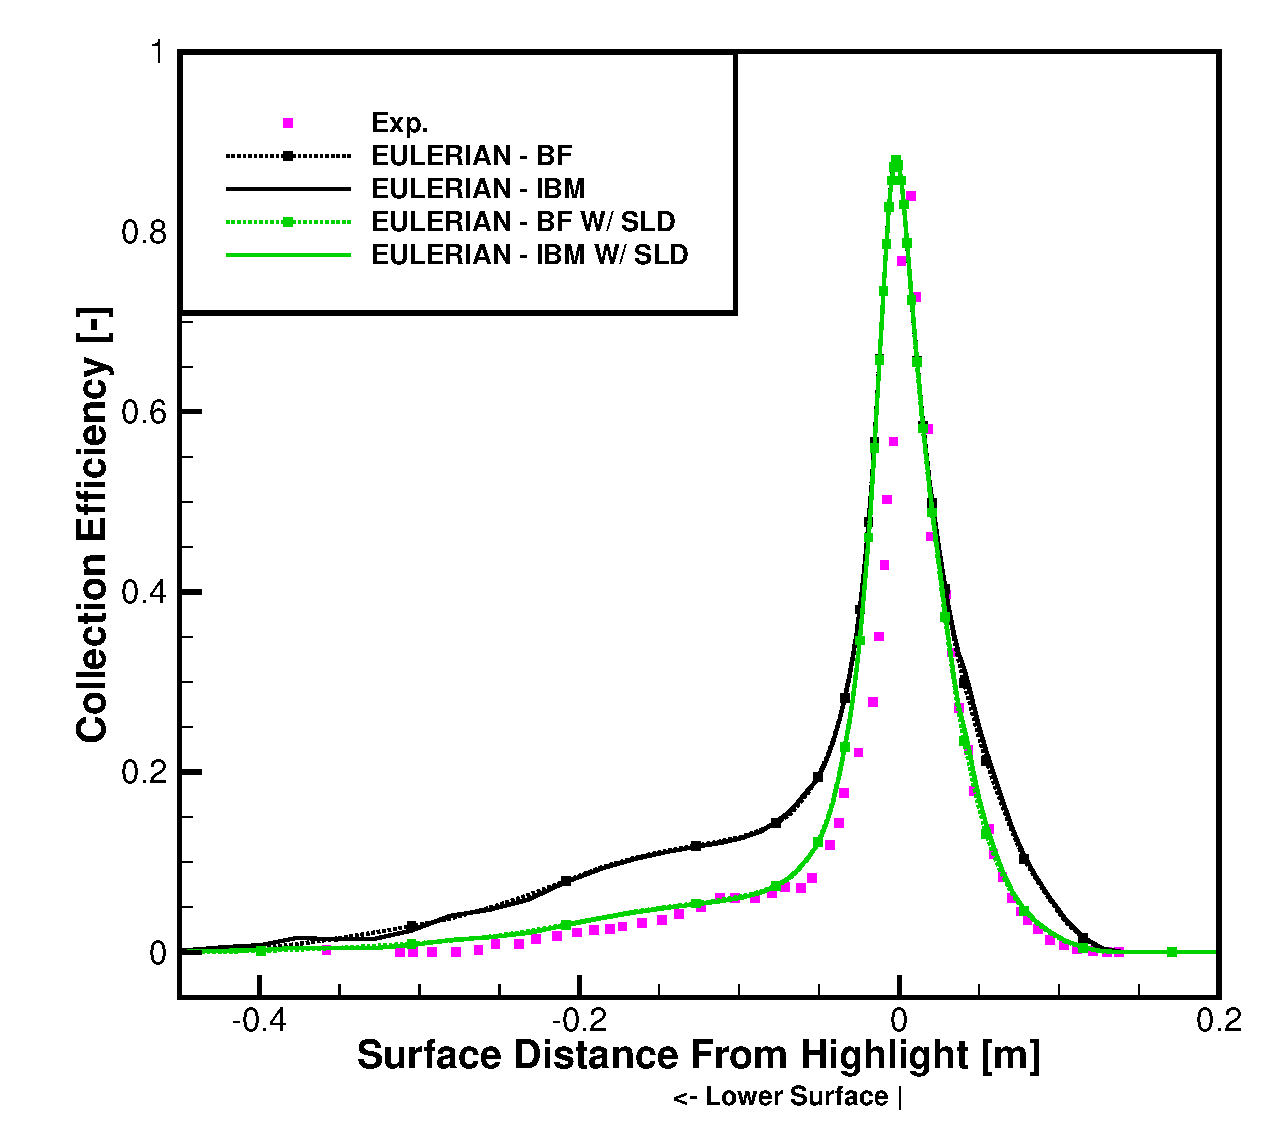
\includegraphics[width=\linewidth,height=4.95cm,keepaspectratio]{FIGURES/IBM/CASE_SLD_EULERIAN_BETA}
  \end{column}
  \hfill
  \begin{column}{0.49\textwidth}
    \centering
    {\color{champsBlue}\bfseries Lagrangian}\par\vspace{0.08cm}
    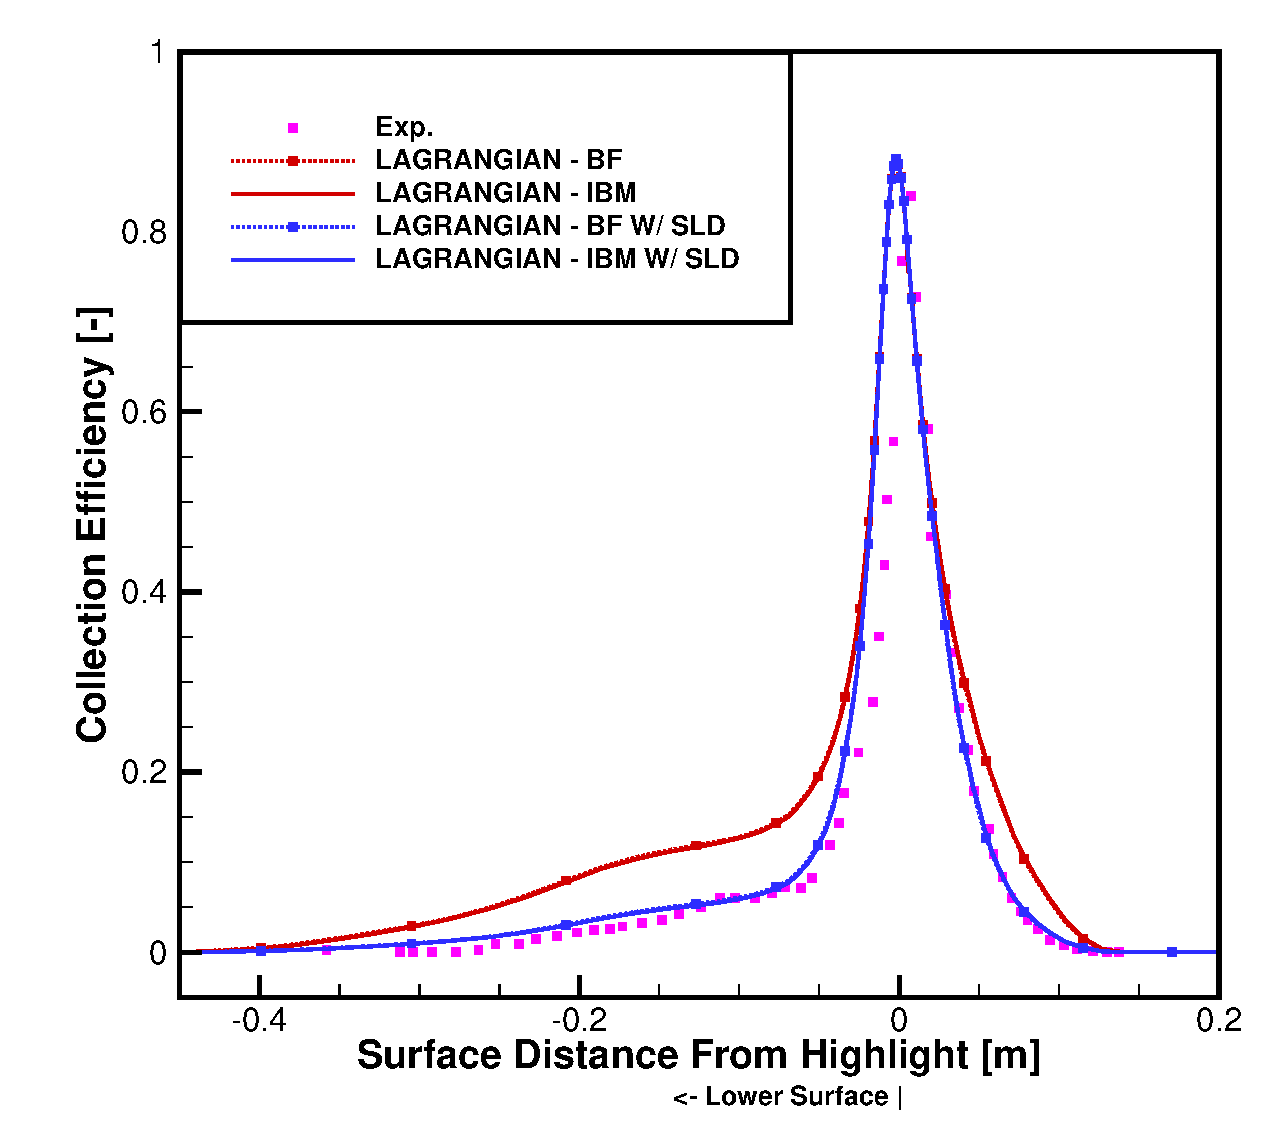
\includegraphics[width=\linewidth,height=4.95cm,keepaspectratio]{FIGURES/IBM/CASE_SLD_LAGRANGIAN_BETA}
  \end{column}
\end{columns}
\vspace{-0.15cm}
\begin{center}

\begin{tikzpicture}
\node[fill=champsBlue!5, draw=champsBlue!18, rounded corners=4pt,
      text width=0.92\textwidth, inner sep=3pt, align=center, font=\small] {%
\textbf{BF and IBM agree closely} for both droplet formulations;
SLD splashing corrections improve experimental agreement.};
\end{tikzpicture}
\end{center}
\SlideRef{papadakis2007large}
\end{frame}

% 6. NACA0012 RIME
\begin{frame}[t]{IBM Ice Accretion Results: Rime (Case 01)}
\vspace{0.06cm}
\begin{center}
{\scriptsize\color{champsBlue}\bfseries NACA 0012 \quad
$\bm{M_\infty=0.325}$ \quad \textbf{AoA} $\bm{=4^\circ}$ \quad
LWC $=0.60$ g/m$^3$ \quad MVD $=20\,\mu$m \quad Exposure time $=420$ s}
\end{center}
\vspace{-0.15cm}
\begin{columns}[c,onlytextwidth]
\begin{column}{0.61\textwidth}
\centering
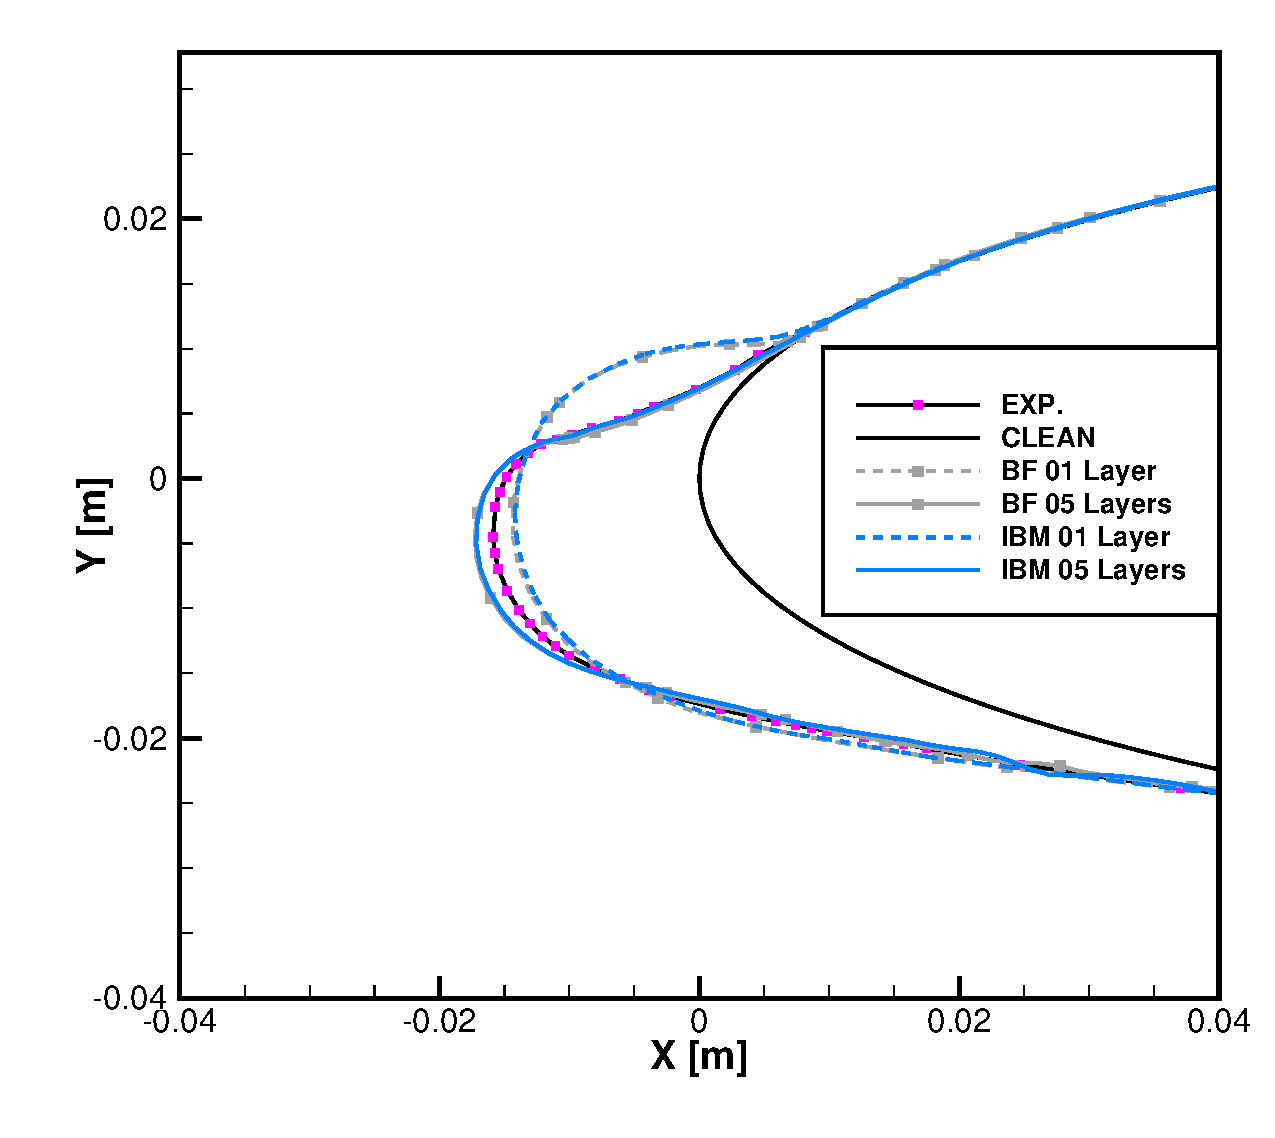
\includegraphics[width=\linewidth,height=5.3cm,keepaspectratio]{FIGURES/IBM/CASE_01_ICE_SHAPE}
\end{column}
\hfill
\begin{column}{0.36\textwidth}
{\color{champsBlue}\bfseries Main Observations}\par
\vspace{0.08cm}
\begin{itemize}\setlength{\itemsep}{5pt}
  \item Close \textbf{BF--IBM agreement}.
  \item Good agreement with experiments.
  \item Five-layer prediction improves over single-step.
\end{itemize}
\end{column}
\end{columns}
\vfill
\begin{center}

\begin{tikzpicture}
\node[fill=champsBlue!5, draw=champsBlue!18, rounded corners=4pt,
      text width=0.92\textwidth, inner sep=3pt, align=center, font=\small] {%
\textbf{Impingement-driven ice accretion (rime cases) is very well predicted with the IBM.}};
\end{tikzpicture}
\end{center}
\end{frame}

% 7. NACA0012 GLAZE / HTC
\begin{frame}[t]{IBM Ice Accretion Results: Glaze (Case 04)}
\vspace{-0.3cm}
\begin{center}
{\scriptsize\color{champsBlue}\bfseries NACA 0012 \quad
$\bm{M_\infty=0.317}$ \quad \textbf{AoA} $\bm{=4^\circ}$ \quad
LWC $=0.55$ g/m$^3$ \quad MVD $=15\,\mu$m \quad Exposure time $=384$ s}
\end{center}
\vspace{-0.1cm}
\begin{columns}[T,onlytextwidth]
  \begin{column}{0.495\textwidth}
    \centering {\color{champsBlue}\bfseries Five-Layer Ice Shape}\par\vspace{0.06cm}
    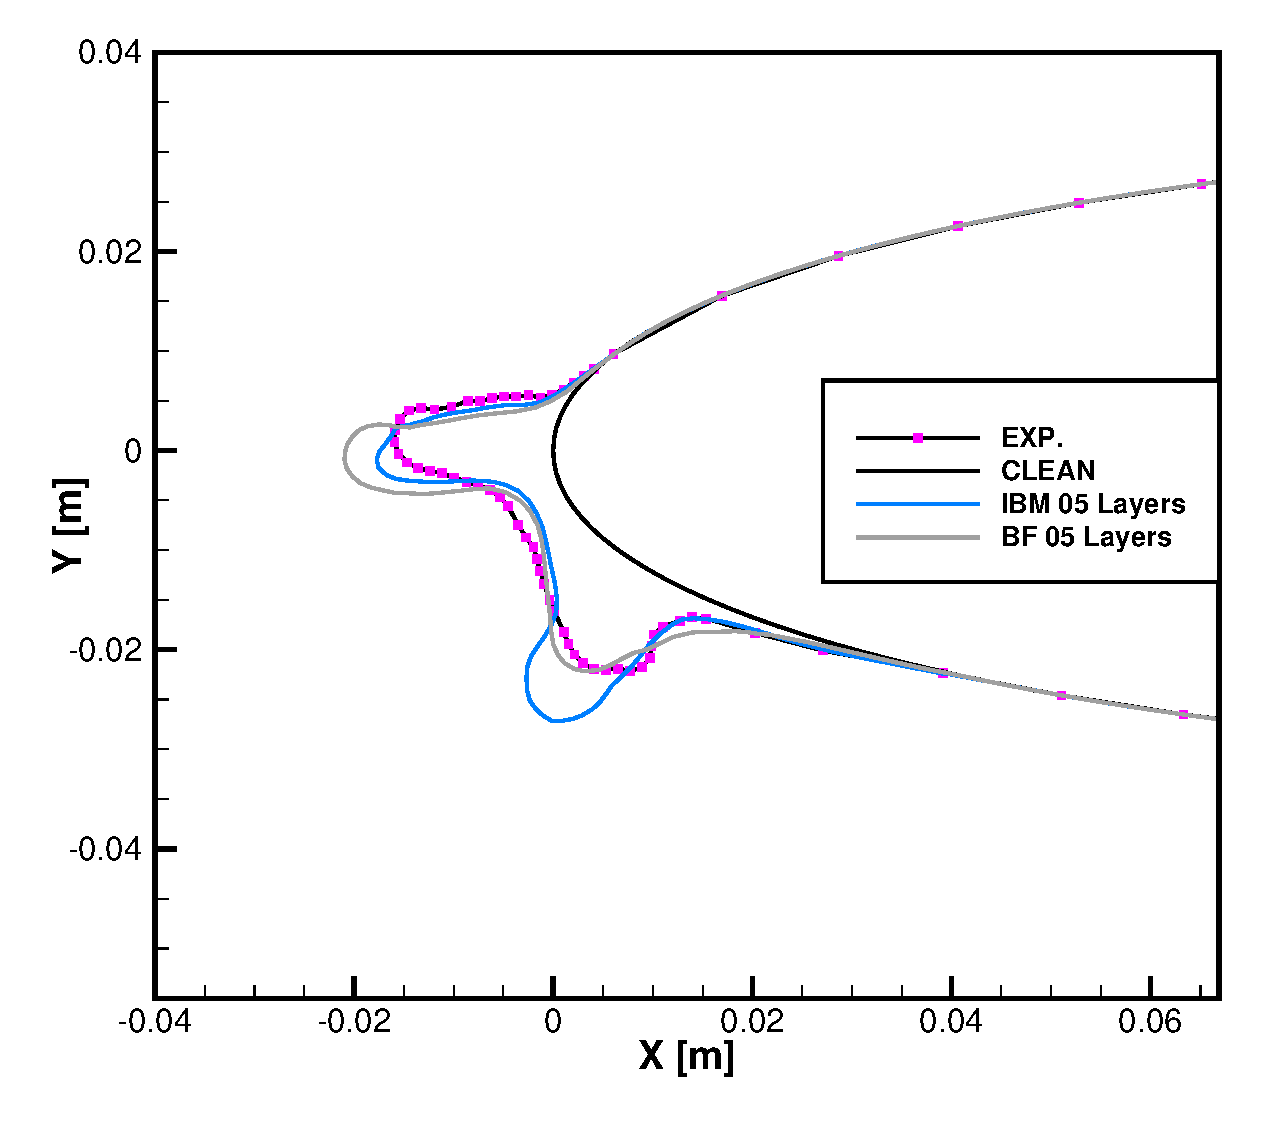
\includegraphics[width=\linewidth,height=5.45cm,keepaspectratio]{FIGURES/IBM/CASE_04_ICE_SHAPE_05_LAYER}
  \end{column}
  \hfill
  \begin{column}{0.495\textwidth}
    \centering {\color{champsBlue}\bfseries Convective Heat Transfer}\par\vspace{0.06cm}
    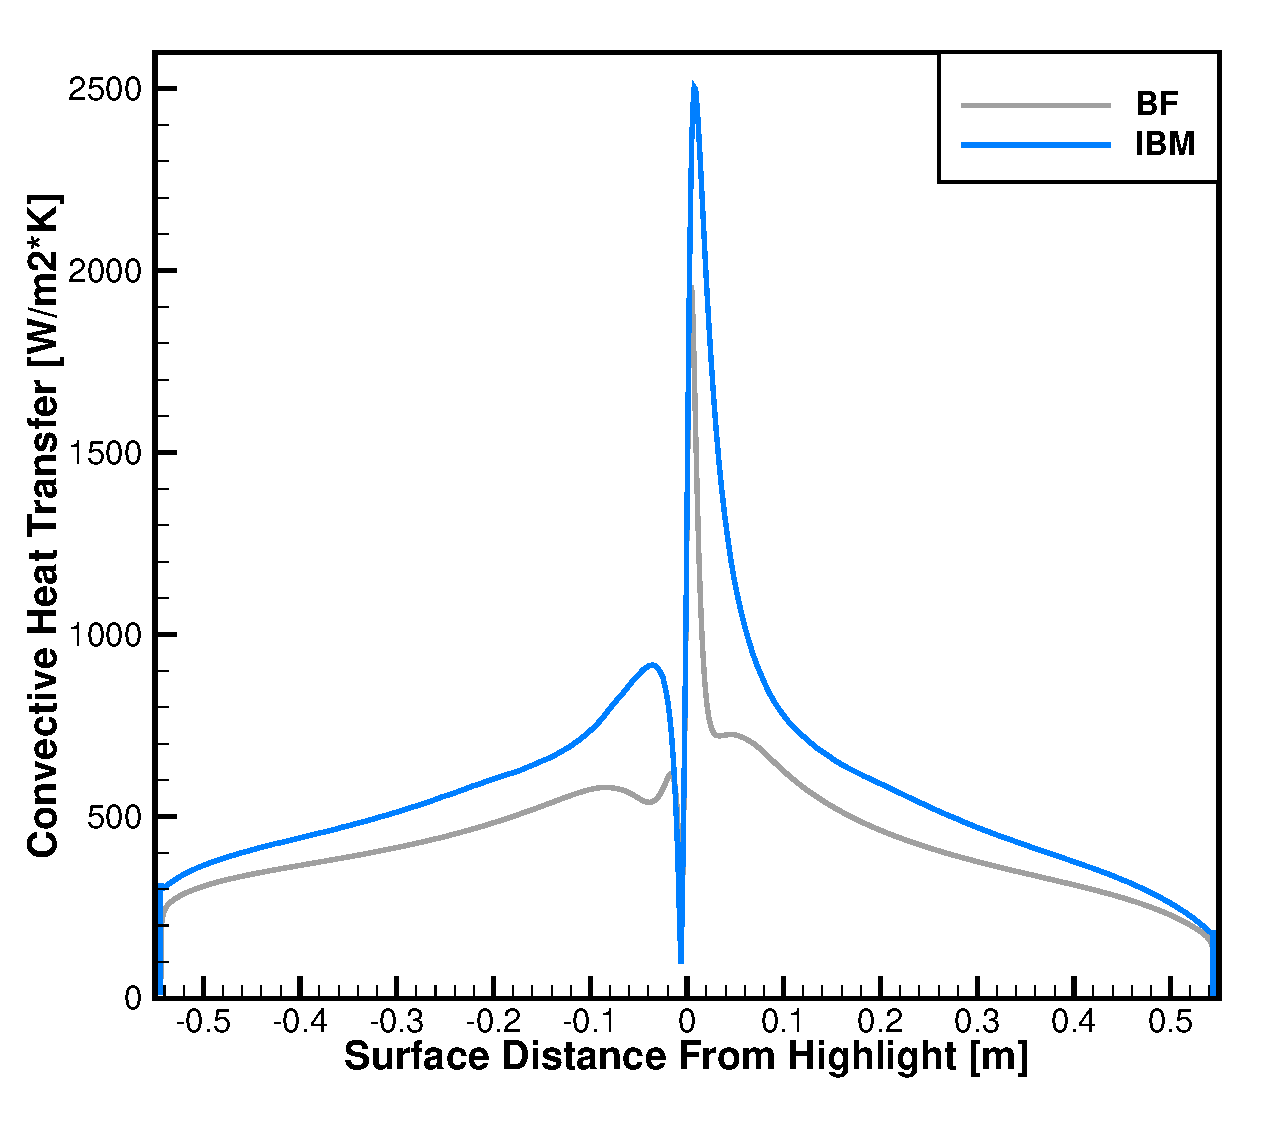
\includegraphics[width=\linewidth,height=5.45cm,keepaspectratio]{FIGURES/IBM/CASE_04_HTC}
  \end{column}
\end{columns}
\vspace{-0.2cm}
\begin{center}
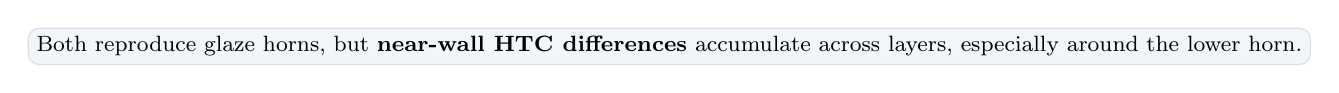
\begin{tikzpicture}
\node[fill=champsBlue!5, draw=champsBlue!18, rounded corners=4pt,
      minimum width=0.98\textwidth, inner sep=3pt, font=\footnotesize] {%
Both reproduce glaze horns, but \textbf{near-wall HTC differences} accumulate across layers, especially around the lower horn.};
\end{tikzpicture}
\end{center}
\end{frame}


\section[Conclusions]{Conclusions and Perspectives}

% Section transition: 06_CONCLUSIONS_AND_PERSPECTIVES
\begin{frame}[plain]
\begin{tikzpicture}[remember picture,overlay]
\shade[left color=white,right color=iceBlue!25]
  (current page.south west) rectangle (current page.north east);
\node[text=champsBlue!70!black,align=center,
  font=\fontsize{26}{32}\selectfont\bfseries]
  (t) at (current page.center) {Conclusions\\ \& \\ Perspectives};
\shade[left color=champsBlue!0,right color=champsBlue]
  ([xshift=-3cm,yshift=-0.45cm]t.south) rectangle ([xshift=-1cm,yshift=-0.5cm]t.south);
\fill[champsBlue] ([xshift=-1cm,yshift=-0.43cm]t.south) rectangle ([xshift=1cm,yshift=-0.52cm]t.south);
\shade[left color=champsBlue,right color=champsBlue!0]
  ([xshift=1cm,yshift=-0.45cm]t.south) rectangle ([xshift=3cm,yshift=-0.5cm]t.south);
\end{tikzpicture}
\end{frame}


\begin{frame}{General Conclusions}

\vspace{0.15cm}

{\color{champsBlue}\bfseries
Lagrangian Droplet Impingement}

\vspace{0.10cm}

\begin{itemize}
    \item Efficient and scalable particle tracking,
    with adaptive seeding and accelerated intersections.
    \item Consistent Eulerian--Lagrangian predictions,
    with extended capabilities for SLD modeling.
\end{itemize}

\vspace{0.22cm}

{\color{champsBlue}\bfseries
Three-Dimensional Level-Set Ice Accretion}

\vspace{0.10cm}

\begin{itemize}
    \item Robust multilayer geometry evolution,
    avoiding surface-mesh entanglement.
    \item Successful prediction of complex 3D ice
    morphologies, including scallop structures.
\end{itemize}

\vspace{0.22cm}

{\color{champsBlue}\bfseries
Immersed Boundary Method}

\vspace{0.10cm}

\begin{itemize}
    \item Integration of flow, droplet, thermodynamic,
    and geometry-evolution models.
    \item Demonstrated feasibility of ice accretion
    without repeated body-fitted aerodynamic remeshing.
\end{itemize}

\vfill

\begin{center}
\colorbox{champsBlue!7}{%
\parbox{0.92\textwidth}{%
\centering
\small\bfseries
A robust numerical foundation for increasingly
complex 3D multilayer ice-accretion simulations.
}}
\end{center}

\end{frame}

\begin{frame}{Current Limitations}

\vspace{0.22cm}

{\color{champsBlue}\bfseries
Physical Modeling}

\vspace{0.10cm}

\begin{itemize}
    \item Ice-shape accuracy remains sensitive to
    aerodynamic, thermodynamic, and droplet predictions.
    \item Glaze ice is particularly sensitive to
    heat-transfer and surface-roughness modeling.
\end{itemize}

\vspace{0.35cm}

{\color{champsBlue}\bfseries
Lagrangian Computational Cost}

\vspace{0.10cm}

\begin{itemize}
    \item Converged 3D impingement fields may require
    large numbers of trajectories.
    \item Irregular workloads and memory access
    complicate distributed-memory scalability.
\end{itemize}

\vspace{0.35cm}

{\color{champsBlue}\bfseries
Immersed Boundary Method}

\vspace{0.10cm}

\begin{itemize}
    \item Absence of adaptive mesh refinement (AMR).
    \item Large predefined refined regions may
    increase computational cost.
    \item Near-wall heat-transfer modeling
    requires further improvement.
\end{itemize}

\end{frame}

\begin{frame}{Future Perspectives}

\vspace{0.20cm}

\begin{columns}[T,onlytextwidth]

% LEFT COLUMN
\begin{column}{0.48\textwidth}

{\color{champsBlue}\bfseries
Physical Modeling}

\vspace{0.12cm}

\begin{itemize}
    \item Spatially and temporally varying
    surface roughness.
    \item Variable ice-density models.
    \item Improved thermodynamic
    and heat-transfer predictions.
\end{itemize}

\vspace{0.35cm}

{\color{champsBlue}\bfseries
Level-Set Geometry Evolution}

\vspace{0.12cm}

\begin{itemize}
    \item Accelerate MMG surface extraction
    and improve mesh quality.
    \item Investigate local ice-mass
    conservation strategies.
\end{itemize}

\end{column}

% RIGHT COLUMN
\begin{column}{0.48\textwidth}

{\color{champsBlue}\bfseries
Immersed Boundary Method}

\vspace{0.12cm}

\begin{itemize}
    \item Adaptive mesh refinement
    around the evolving ice interface.
    \item Improved near-wall
    heat-transfer treatment.
\end{itemize}

\vspace{0.35cm}

{\color{champsBlue}\bfseries
Lagrangian Droplet Tracking}

\vspace{0.12cm}

\begin{itemize}
    \item GPU acceleration for
    large-scale 3D simulations.
    \item Improved data locality
    and workload balancing.
\end{itemize}

\end{column}

\end{columns}

\vfill

\begin{center}
\colorbox{champsBlue!7}{%
\parbox{0.92\textwidth}{%
\centering
\small\bfseries
Toward more accurate, efficient, and automated
3D multilayer ice-accretion simulations.
}}
\end{center}

\end{frame}



\begin{frame}{Acknowledgments}

\begin{itemize}
    \item This work is supported in part by a Bombardier/NSERC/CRIAQ Industrial Chair.

    \item Computations were performed on the Trillium supercomputer at the SciNet HPC Consortium, with computational resources provided through the Digital Research Alliance of Canada.

    %\item SciNet is funded by Innovation, Science and Economic Development Canada; the Digital Research Alliance of Canada; the Ontario Research Fund: Research Excellence; and the University of Toronto.
\end{itemize}

\end{frame}


\nocite{clift2005bubbles,OSHER2004,FROLKOVIC2015214,lavoieLevelSet,alessandroLevelSet,dapogny2014mmg}
\setbeamertemplate{frametitle continuation}{}
\begin{frame}[allowframebreaks]{References}
\footnotesize
\bibliography{references}
\end{frame}

\end{document}
